\documentclass{puthesis-UG}

\usepackage{style}

%%%%%%%%IMPORTANT INFORMATION%%%%%%%%%%%%%%%%%%%%
%Using puthesis-UG.cls includes an Honor Code declaration. By using this file you are 
%declaring that this paper is your own work in accordance with University retgulations.
%
%The file puthesis-UG.cls must be downloaded from the math department website and 
%saved in the same directory as this file.
%%%%%%%%%%%%%%%%%%%%%%%%%%%%%%%%%%%%%%%%

\author{Alan Yan}
\adviser{Professor June E. Huh}
\title{Hodge-Riemann Relations of the Basis Generating Polynomial of a Matroid}
\abstract{(write something flowery)}
\acknowledgements{I would like to thank}
\date{today}


% Things I want to talk about:

% 1. Combinatorial Atlas
% 2. Lorentzian Polynomials
% 3. Alexandrov-Fenchel Inequality
% 4. 
%


\begin{document}
 
\chapter{Conventions and Notation}

\chapter{Introduction}

\chapter{Preliminaries: Combinatorial Structures and Convex Geometry}

\section{Partially Ordered Sets}

Our main reference for partially ordered sets is \cite{ordered-sets}. 
\begin{defn}
	A \textbf{partially ordered set} is an ordered pair $(P, \leq)$ of a set $P$ and a binary relation $\leq$ on $P$ such that 
	\begin{enumerate}
		\item[(\textbf{P1})] $x \leq x$ for all $x \in P$. 
		\item[(\textbf{P2})] If $x \leq y$ and $y \leq x$, then $x = y$. 
		\item[(\textbf{P3})] If $x \leq y$ and $y \leq z$, then $x \leq z$. 
	\end{enumerate}
\end{defn}

\begin{example}
	We provide a list of exmaples of common posets which appear naturally in mathematics. 
	\begin{enumerate}[label = (\alph*)]
		\item Any subset of the real numbers equipped with the less-than-or-equal-to relations $\leq$.
		\item Any subset of the integers equipped with the divisibility relation.
		\item Any collection of sets equipped with the inclusion relation. 
		\item The vertices of a directed graph where $v \leq w$ if and only if $w$ can be reached from a directed path started at $v$. 
	\end{enumerate}
\end{example}

\subsection{Linear Extensions}

\begin{defn}
	Let $(P, \leq)$ be a poset on $n$ elements. A \textbf{linear extension} is any bijective map $f : P \to [n]$ satisfying $f(x) < f(y)$ for all $x, y \in P$ satisfying $x < y$.
\end{defn}
\subsection{Lattices}

\begin{defn}
	We say a poset $\mcL$ is a lattice if for any $x, y \in \mcL$ there exist (unique) poset elemenets $x \vee y$ (called the \textbf{meet} or \textbf{greatest lower bound}) and $x \wedge y$ (called the \textbf{join} or \textbf{least upper bound}) satisfying 
	\begin{enumerate}
		\item[(\textbf{L1})] $x \vee y \geq x$, $x \vee y \geq y$, and for any $z \in \mcL$ satisfying $z \geq x$ and $z \geq y$, we have $z \geq x \vee y$. 
		\item[(\textbf{L2})] $x \wedge y \leq x$, $x \wedge y \leq y$, and for any $z \in \mcL$ satisfying $z \leq x$ and $z \leq y$, we have $z \leq x \wedge y$. 
	\end{enumerate}
\end{defn}

The only lattice that we will be concerned with are geometric lattices. 
\section{Graph Theory}

We assume a working knowledge of basic graph theory. This includes concepts such as connected components, paths, trees, etcetera. We provide the definition of a graph that we will use in this paper. Note that we allow multi-edges and but not loops. This is because in later results concerning graphic matroids, the presense of loops does not affect log-concavity. Our main reference for basic notions in graph theory come from \cite{diestel}. For more the more sophistication notions that come from spectral graph theory, we refer to \cite{chung-spectral-graph-theory}. 

\begin{defn}
	A \textbf{graph} is an ordered pair $(V, E)$ of vertices and edges such that each edge is associated with either two distinct vertices or one vertex. If an edge is associated with two distinct vertices, then we call it a \textbf{simple edge}. If an edge is associated with one vertex, then we call it a \textbf{loop}. 
\end{defn}

\subsection{Spectral Graph Theory}

\begin{defn}
	Given a graph $G$ with $n$ vertices $v_1, \ldots, v_n$, we define its Laplacian matrix $L := L_G$ to be the $n \times n$ matrix defined element-wise as 
	\[
		L_{i, j} := \begin{cases}
			\deg (v_i) & \text{if $i = j$} \\
			-E_{v_i, v_j} & \text{if $i \neq j$ and $v_i$ is adjacent to $v_j$}
		\end{cases}
	\]
	where $E_{v_i, v_j}$ is the number of edges between $v_i$ and $v_j$. 
\end{defn}

\begin{defn}
	Let $G$ be a graph and let $V = \{v_1, \ldots, v_n\}$ be an arbitrary ordering of the vertices. For this ordering, we can define a $|V| \times |E|$ matroid $B_G$ called the \textbf{incidence matrix} where the entry indexed by $v \in V$ and $e = \{v_i, v_j\} \in E$ where $v_i > v_j$ is equal to 
	\[
		B_{ve} = \begin{cases}
			1, & \text{if $v = v_i$} \\
			-1, & \text{if $v = v_j$} \\
			0, & \text{otherwise.}
		\end{cases}
	\]
	The matrix $C_G$ which is obtained by removing the last row of $B_G$ is called the \textbf{reduced incidence matrix}. 
\end{defn}

The incidence matrix and reduced incidence matrix satisfy the condition in Proposition~\ref{incidence-reduced-incidence-matrix-is-good}. This connects the linear independence of the columns of the incidence matrices of $G$ to the cyclelessness of subgraphs of $G$. This proposition will provide an example of the combinatorial structure of a matroid introduced in the subsequent section. 

\begin{prop} \label{incidence-reduced-incidence-matrix-is-good}
	For a graph $G = (V, E)$ the incidence matrix $B_G$ and reduced incidence matrix $C_G$ both satisfy the property that a set of columns are linearly independent if and only if the graph formed by the corresponding edges does not contain a cycle. 
\end{prop}

\begin{proof}
	See Example 5.4 of \cite{bapat_raghavan_1997}. 
\end{proof}

\begin{prop} \label{incidence-and-laplacian-relation-prop}
	Let $G$ be a graph and $L$ be its Laplacian. Then, for any arbitrary ordering on the vertices, we have that $L = B B^T$. 
\end{prop}

\begin{proof}
	For each $e = \{v_i, v_j\} \in E$ with $v_i > v_j$, we define $\pi_e(v_i) = 1$ and $\pi_e (v_j) = -1$. We have that 
	\[
		(BB^T)_{v, w} = \sum_{e \in E : v, w \in e} \pi_e(v) \pi_e(w). 
	\]
	When $v = w$, then each summand is equal to $1$ and we get exactly $\deg (v_i)$. If $v$ and $w$ are not adjacent, then the sum is empty and the netry is equal to zero. Otherwise, each summand is $-1$ and there are $E_{v_i, v_j}$ elements in this sum. This suffices for the proof of the proposition. 
\end{proof}

\section{Matroids}

Matroids can be thought of as combinatorial objects which abstracts and generalizes the properties of both linear independence in vectors spaces and cyclelessness in graphs. Despite the seemingly limited scope of this interpretation, matroids successfully describe many objects relevant to other areas in mathematics such as topology \cite{gelfand}, graph theory \cite{milnor-numbers}, combinatorial optimization \cite{optimization}, algebraic geometry \cite{schubert-cell}, and convex geometry \cite{matroid-polytope}. In this subsection, we provide an introduction to the basic notions in matroid theory that we will need in the remainder of this thesis. We use the excellent monographs \cite{10.5555/1197093} and \cite{welsh} as our main references for the basic theory.

\subsection{Independent Sets}
\begin{defn}
	A \textbf{matroid} is an ordered pair $M = (E, \mcI)$ consisting of a finite set $E$ and a collection of subsets $\mathcal{I} \subseteq 2^E$ which satisfy the following three properties:
	\begin{enumerate}
		\item[(\textbf{I1})] $\emptyset \in \mathcal{I}$. \footnote{(\textbf{I1}) is the \textbf{non-emptiness} axiom}
		\item[(\textbf{I2})] If $X \subseteq Y$ and $Y \in \mathcal{I}$, then $X \in \mathcal{I}$.\footnote{(\textbf{I2}) is the \textbf{hereditary} axiom}
		\item[(\textbf{I3})] If $X, Y \in \mathcal{I}$ and $|X| > |Y|$, then there exists some element $e \in X \backslash Y$ such that $Y \cup \{e\} \in \mathcal{I}$. \footnote{(\textbf{I3}) is the \textbf{exchange} axiom}
	\end{enumerate}
	The set $E$ is called the ground set of the matroid and the collection of subsets $\mathcal{I}$ are called independent sets. This naming convention is motivated by Example~\ref{linear-matroid} where the indepedent sets consist exactly of sets of linearly independent vectors. 
\end{defn}

\begin{example} [Linear Matroids] \label{linear-matroid}
	Let $V$ be a $k$-vector space and let $E = \{v_1, \ldots, v_n\}$ be a finite set of vectors from $V$. If we let $\mcI$ consist of all subsets of $E$ which are linearly independent, then $(E, \mcI)$ forms a matroid. We call any matroid which can be constructed in this way a \textbf{linear matroid}. 
\end{example}

\begin{example} [Graphic Matroids]
	Let $G = (V, E)$ be a graph and let $\mcI$ be the collection of subsets of $E$ which consist of edges containing no cycles. Then $(E, \mcI)$ forms a matroid called the \textbf{cycle matroid} of the graph $G$. We call any matroid which is isomorphic to a cycle matroid of a graph a \textbf{graphic matroid}. In Proposition~\ref{graphic-are-linear}, we prove that graphic matroids are not only linear, but they can be represented by a totally unimodular matrix. 
\end{example}
\begin{prop} \label{graphic-are-linear}
	
\end{prop}

\begin{example}[Uniform Matroids]

\end{example}


Given a matroid $M = (E, \mathcal{I})$, we call a subset $X \subseteq E$ a \textbf{dependent set} if and only if $X \notin \mathcal{I}$. Given a matroid, we call any minimal dependent set a \textbf{circuit}. Matroids are uniquely determined by their circuits. For a proof of this fact, see Corollary 1.1.5 in \cite{10.5555/1197093}.

\subsection{Bases}
We define a basis $B \in \mathcal{I}$ to be a maximal independent set. From property (\textbf{I3}), we can deduce that all bases have the same number of elements. Indeed, if $B_1$ and $B_2$ are bases satisfying $|B_1| < |B_2|$ then from (\textbf{I3}) there exists some element $e \in B_2 \backslash B_1$ satisfying $B_1 \cup \{e\} \in \mcI$. But, this means that $B_1 \cup \{e\}$ is an independent set strictly larger than $B_1$. This contradicts the maximality of $B_1$ and implies that all bases contain the same number of elements. 
\begin{defn}
	Let $M = (E, \mathcal{I})$ be a matroid and let $\mcB$ be the collection of bases. Then, the following three properties (Lemma 1.2.2 in \cite{10.5555/1197093}):
	\begin{enumerate}
		\item[\textbf{(B1)}] $\mcB$ is non-empty.
		\item[\textbf{(B2)}] If $B_1$ and $B_2$ are members of $\mcB$ and $x \in B_1 \backslash B_2$, then there is an element $y$ of $B_2 \backslash B_1$ such that $(B_1 - x) \cup y \in \mcB$. 
		\item[\textbf{(B3)}] If $B_1$ and $B_2$ are members of $\mcB$ and $x \in B_1 \backslash B_2$, then there is an element of $y \in B_2 \backslash B_1$ such that $(B_2 - y) \cup x \in \mcB$. 
	\end{enumerate}
\end{defn}

Associated with the bases of a matroid, we can define the \textbf{basis generating function} of a matroid $M = (E, \mcB)$ as
\[
	f_M (x) := \prod_{B \in \mcB} x^B \in \RR[x_e : e \in E]
\]
which is a homomogeneous polynomial in the ring of polynomials with variables indexed by the ground set of our matroid. 

\subsection{Rank Functions}

\begin{defn}
	For any matroid $M = (E, \mcI)$, we define its rank function $\rank_M : 2^E \to \NN$ to be equal to
	\[
		\rank_M(X) := \max \{|I| : I \in \mathcal{I}, I \subseteq X\}.
	\]
	The rank function satisfies the following three properties (Lemma 1.3.1 in \cite{10.5555/1197093}):
	\begin{enumerate}
		\item[(\textbf{R1})] If $X \subseteq E$, then $0 \leq r(X) \leq |X|$. 
		\item[(\textbf{R2})] If $X \subseteq Y \subseteq E$, then $r(X) \leq r(Y)$. 
		\item[(\textbf{R3})] If $X$ and $Y$ are subsets of $E$, then $r(X \cup Y) + r(X \cap Y) \leq r(X) + r(Y)$.
	\end{enumerate}
\end{defn}


\subsection{Closure Operators and Lattice of Flats}

\begin{defn}
	For any matroid $M = (E, \mcI)$, we define its closure operator $\clo_M : 2^E \to 2^E$ to be 
	\[
		\clo_M (X) := \overline{X} = \{x \in E : \rank (X \cup \{x\}) = \rank (X) \}.
	\]
	The closure operator satisfies the following four properties (Lemma 1.4.3 in \cite{10.5555/1197093}):
	\begin{enumerate}
		\item[(\textbf{C1})] If $X \subseteq E$, then $X \subseteq \clo_M (X)$. 
		\item[(\textbf{C2})] If $X \subseteq Y \subseteq E$, then $\clo_M (X) \subseteq \clo_M (Y)$. 
		\item[(\textbf{C3})] If $X \subseteq E$, then $\clo_M (\clo_M(X)) = \clo_M(X)$. 
		\item[(\textbf{C4})] If $X \subseteq E$ and $x \in E$, and $y \in \clo_M(X \cup \{x\}) \backslash \clo_M(X)$, then $x \in \clo_M(X \cup \{y\})$. 
	\end{enumerate}
\end{defn}

\begin{example}
	Let $M := M(\{v_1, \ldots, v_n\})$ be the linear matroid represented by vectors $v_1, \ldots, v_n$ in a $k$-vector space $V$. Then, the closure of a subset $X \subseteq \{v_1, \ldots, v_n\}$ is precisely $\clo_M(X) := \{v_1, \ldots, v_n\} \cap \mathsf{span}_k X$. 
\end{example}

If $X \subseteq E$ satisfies $X = \clo_M(X)$, then we say $X$ is a \textbf{closed set} or \textbf{flat}. For any matroid $M = (E, \mcI)$, let $\mcL(M)$ denote the partially ordered set consisting of the flats of $M$ equipped with set inclusion. 

\begin{prop}[Theorem 1.7.5 in \cite{10.5555/1197093}]
	Let $M = (E, \mcI)$ be a matroid. Then, the poset $\mcL(M)$ is a geometric lattice with join and meet operations defined as $X \vee Y := \clo_M(X \cup Y)$, $X \wedge Y := X \cap Y$, and rank function $\rank_{\mcL} (X) := \rank_M(X)$. 
\end{prop}


\subsection{Loops and Parallel Elements}
We say $e \in E$ is a \textbf{loop} in $M$ if $\{e\}$ is a dependent set. Equivalently, $e \in E$ is a loop if $\rank (\{e\}) = 0$. We define $E_0$ as the set of loops. An element $e \in E$ in the ground set is called a \textbf{coloop} if it is contained in every basis. We say $x_1, x_2 \in E \backslash E_0$ satisfy $x_1 \sim_M x_2$ if and only if $\{x_1, x_2\} \notin \mcI$ or $x_1 = x_2$. Equivalently, $x_1 \sim_M x_2$ if and only if $\rank (\{x_1, x_2\}) = 1$. When $x_1 \sim_M x_2$, we say that $x_1$ and $x_2$ are \textbf{parallel}. For a more in-depth treatment of loops and parallelism, I refer the reader to section 1.4 of \cite{welsh}.

\begin{prop} \label{parallelism-is-equivalence-relation}
	Let $M = (E, \mcI)$ be a matroid. Then $\sim_M$ is an equivalence relation on $E \backslash E_0$. 
\end{prop}

\begin{proof}
	For any $x \in E \backslash E_0$, we have $\rank (\{x, x\}) = \rank (\{x\}) = 1$ since $x \notin E_0$. Thus $x \sim_M x$. For $x, y \in E \backslash E_0$, we have $\rank (\{x, y\}) = \rank \{y, x\}$. This proves that $\sim_M$ is reflexive. To prove transitivity, suppose that we have $x, y, z \in E$ that satisfy $x \sim_M y$ and $y \sim_M z$. If $x = y$ or $y = z$, then we automatically get $x \sim_M z$. Suppose that they are all distinct. Then, we have $\{x, y\}, \{y, z\} \not\in \mcI$. For the sake of contradiction, suppose that $\{x, z\} \in \mcI$. From (\textbf{I3}) applied to $\{x, z\}$ and $\{y\}$, we have that either $\{x, y\} \in \mcI$ or $\{y, z\} \in \mcI$. This is a contradiction. This proves that $\sim_M$ is transitive and an equivalence relation. 
\end{proof}

From Proposition~\ref{parallelism-is-equivalence-relation}, for any non-loop $e \in E \backslash E_0$, we can consider its equivalence class $[e] := [e]_M$ under the equivalence relation $\sim_M$. We call the equivalence class $[e]$ the \textbf{parallel class} of $e$. Then, we can partition the ground set $E$ into $E = E_1 \sqcup E_2 \sqcup \ldots \sqcup E_s \sqcup E_0$ where $E_1, \ldots, E_s$ are the distinct parallel classes and $E_0$ are the loops. In Proposition~\ref{characterization-of-atoms-of-flats}, we give a characterization of the atoms of the lattice of flats in terms of the parallel classes and loops. 

\begin{prop} \label{characterization-of-atoms-of-flats}
	Let $M = (E, \mcI)$ be a matroid and let $e \in E$ be an element of the matroid that is not a loop. Then, $\overline{e} = [e] \cup E_0$.
\end{prop}

\begin{proof}
	Since any independent set contains no loops, we know that $E_0 \subseteq \overline{e}$. For any $f \in [e]$, we have that $\rank (\{e, f\}) = 1 = \rank (\{e\})$ by definition of $\sim_M$. This proves that $[e] \subseteq \overline{e}$. To prove the opposite inclusion, let $f \in \overline{e}$. Then $\rank(\{e, f\}) = 1$. If $f$ is a loop, then $f \in E_0$. Otherwise, $f \sim_M e$ and $f \in [e]$. This suffices for the proof of the proposition. 
\end{proof}

We call a matroid $\textbf{simple}$ if it contains no loops and no parallel elements. To every matroid $M$, we can associate a simple matroid $\widetilde{M}$ called the \textbf{simplification} of the matroid $M$. For any matroid $M = (E, \mcI)$, let $\pi_M : E \to 2^E$ be the map $\pi_M (e) = \overline{e}$ which sends a matroid element to its closure. When $e$ is not a loop, then $\overline{e}$ is a one-dimensional flat. If $e$ is a loop, then $\overline{e} = E_0$. From Proposition~\ref{characterization-of-atoms-of-flats}, we can think of $\pi_M (E)$ as the set of one-dimensional flats and the set of loops. 

\subsection{Contraction and Deletion}

In graph theory, there are notions of edge contraction and edge deletion. In Definition, we genealize contraction and deletion from graphs to general matroids. When applying contraction and deletion in the matroid sense to graphic matroids, we recover edge contraction and deletion in graph theory.  

\begin{defn}[Restriction, Contraction, and Deletion]\label{contraction-deletion}
	Let $M = (E, \mcI)$ be a matroid and let $T \subseteq E$ be a subset. We define $M|_T$ to be the restriction of $M$ on $T$ as the matroid on $T$ with independent sets 
	\[
		\mcI (M|_T) := \{I \in \mcI : I \subseteq T\}.
	\]
	The deletion $M \backslash T$ of $T$ from $M$ is then defined to be the restriction $M|_{E \backslash T}$. Let $B_T$ be a basis of $M|_T$. The contraction $M / T$ of the matroid $M$ by $T$ is the matroid on $E \backslash T$ defined by
	\begin{align*}
		\mcI(M/T) & := \{I \subset E \backslash T: I \cup B_T \in \mcI(M) \}.
	\end{align*}
	For a proof of why the definition of $\mcI(M/T)$ is independent of our choice of $B_T$ we refer the reader to Proposition 3.1.7 of \cite{10.5555/1197093}.
\end{defn}

\begin{lem}
	Let $M = (E, \mcB)$ be a matroid with basis generating polynomial $f_M$.
	\begin{enumerate}[label = (\alph*)]
		\item If $e \in E$ is a loop, then $\partial_e f_M = 0$. 
		\item If $e \in E$ is not a loop, then $\partial_e f_M = f_{M/e}$. 
		\item If $e \in E$ is not a coloop, then $f_M = x_e f_{M/e} + f_{M \backslash e}$
	\end{enumerate}
\end{lem}

\begin{proof}
	The first claim follows from the fact that any basis will contain no loops. Hence, for a loop $e \in E$ the variable $x_e$ will not appear in $f_M$. The second claim follows from the fact that the remaining monomials in $\partial_e f_M$ will correspond to sets of the form $B \backslash e$ where $e \in B$ and $B$ is a basis of $M$. This is exactly the set of bases of $M / e$. For the third claim, this follows	because the monomials in $f_M$ which do not contain $x_e$ will correspond to bases of $M$ which do not contain $e$. That is the exactly the bases of $M \backslash e$. This implies that we can write $f_M = x_e p + f_{M \backslash e}$ where $p \in \RR[x_e : e \in E]$ and $p$ contains no monomial with $x_e$. Taking the partial derivative with respect to $x_e$, we get $p = f_{M / e}$ from (a). This suffices for the proof. 
\end{proof}

\subsection{Matroids sum and truncation}

In this subsection, we describe a way to add two matroids to get another matroid. Let $M = (E, \mathcal{I}_M)$ and $N = (F, \mathcal{I}_N)$ be matroids. We define the \textbf{matroid sum} of $M$ and $N$ as the matroid $M+N$ on the set $E \sqcup F$ such that the independent sets of $M+N$ are subsets of $E \sqcup F$ of the form $I \cup J$ where $I \in \mcI_M$ and $J \in \mcI_N$. In other words, we define
\[
	\mcI(M+N) := \{I \cup J : I \in \mcI(M), J \in \mcI(N)\}.
\]

\begin{prop} \label{proposition-matroid-sum-is-well-defined}
	The ordered pair $M+N = (E \sqcup F, \mcI(M+N))$ is a matroid. 
\end{prop}

\begin{proof}
	It is clear that $\mcI(M+N)$ contains the empty set and satisfies the hereditary property. Now suppose that $I_1, I_2 \in \mcI(M)$ and $J_1, J_2 \in \mcI(N)$ satisfies $|I_1 \cup J_1| < |I_2 \cup J_2|$. Then we have that
	\[
		|I_1| + |J_1| = |I_1 \cup J_1| < |I_2 \cup J_2| = |I_2| + |J_2|.
	\]
	Without loss of generality, suppose that $|I_1| < |I_2|$. Then, there is a $e \in I_2 \backslash I_1$ such that $I_1 \cup e \in \mathcal{I}(M)$. This means that there is $e \in (I_2 \cup J_2) \backslash (I_1 \cup J_1)$ satisfying $(I_1 \cup J_1) \cup e \in \mcI(M+N)$. This suffices for the proof. 
\end{proof}

For a matroid $M = (E, \mcI)$, we define $TM$ to be the \textbf{truncation} of $M$. This is the matroid on $M$ where the independent sets are the independent sets of $M$ of rank at most $\rank(M) - 1$.  

\subsection{Regular Matroids}

\begin{defn}
	A \textbf{regular matroid} is a matroid which is isomorphic to a linear matroid with respect to a real matrix which is \textbf{totally unimodular}. In this thesis, we also call such matrices \textbf{unimodular} interchangeably, which is not standard in the literature. A totally unimodular matrix is a matrix for which every square submatrix has determinant in $\{0, -1, 1\}$. 
\end{defn}

\begin{prop} \label{graphic-matroid-is-regular-prop}
	The linear matroid generated by the incidence matrix and reduced incidence matrix of a graph are both unimodular coordinatizations of the graphic matroid corresponding to the graph.  
\end{prop}

\begin{proof}
	It suffices to prove that the incidence matrix is totally unimodular
\end{proof}
\section{Mixed Discriminants}

In this section, we discuss a symmetric multilinear form called the mixed discriminant which arises as the polarization of the determinant. This object will be useful in future sections as it satisfies the log-concavity inequality in Theorem (CITE). Our main reference for the theory of mixed discriminants will come from \cite{bapat_raghavan_1997}. One connection between mixed discriminants and mixed volumes can be seen in the formal similaritiy of Theorem~\ref{polarization-mixed-discriminant} and Theorem (CITE???). A deeper connection can be seen in Alexandrov's original paper \cite{aleksandrov} where he introduces mixed discriminants to proof Theorem (CITE???). 

\begin{defn} \label{defn-mixed-discriminant}
	let $n \geq 1$ be a positive integer. Suppose that for each $k \in [n]$, we are given an $n \times n$ matrix $A^k := (a_{ij}^k)_{i, j = 1}^n$. Then, we define the \textbf{mixed discriminant} of $(A^1, \ldots, A^n)$ as the expression 
	\[
		\mathsf{D}(A^1, \ldots, A^n) := \frac{1}{n!} \sum_{\sigma \in S_n} 
		\det 
		\begin{bmatrix} 
			a_{11}^{\sigma(1)} & \ldots & a_{1n}^{\sigma(n)} \\
			\vdots & \ddots & \vdots \\
			a_{n1}^{\sigma(1)} & \ldots & a_{nn}^{\sigma(n)}
		\end{bmatrix}. = \frac{1}{n!} \sum_{\sigma \in S_n} \text{Det}(v^{\sigma(1)}_{1}, \ldots, v_{n}^{\sigma(n)}).
	\]
	Here, $S_n$ is the symmetric group on $n$ letters. 
\end{defn}

From Definition~\ref{defn-mixed-discriminant}, it is clear that the mixed discriminant is multilinear and symmetric in its entries. 

\subsection{Polarization form of a homogeneous polynomial}

Let $f \in \RR[x_1, \ldots, x_n]$ be an arbitrary homogeneous polynomial of degree $d$. Then, for a fixed choice of vectors $v_1, \ldots, v_d \in \RR^n$ we can study the coefficients of the homogeneous polynomial in $\lambda_1, \ldots, \lambda_d$ of the polynomial $f(\lambda_1 \cdot v_1 + \ldots + \lambda_d \cdot v_d)$. We will discuss the notion of the \textbf{polarization form} of a homogeneous polynomial. The notion of the \textbf{polarization form}, also referred to as the \textbf{complete homogeneous form}, is briefly mentioned in section 3.2 of \cite{lie-groups}, section 5.5 of \cite{schneider_2013}, and section 4.1 of \cite{lorentzian-polynomials}. 
\begin{defn}
	Let $k$ be a field of characteristic $0$. Let $f \in k[x_1, \ldots, x_n]$ be a homogeneous polynomial of degree $d$. We define the \textbf{polarization form} or \textbf{complete homogeneous form} of $f$ to be the function $F_f : (k^n)^d \to k$ defined by 
	\[
		F_f (v_1, \ldots, v_d) := \frac{1}{d!} \frac{\partial}{\partial x_1} \ldots \frac{\partial}{\partial x_d} f(x_1 v_1 + \ldots + x_d v_d).
	\]
	This form is multi-linear and symmetric in its arguments. Moreover, $F_f(v, \ldots, v_n) = f(v)$ for all $v \in k^n$. 
\end{defn}

Let $f \in k[x_1, \ldots, x_n]$ be a homogeneous polynomial of degree $d$. Then, we can write this polynomial in the form 
\[
	f(x_1, \ldots, x_n) = \sum_{(\alpha_1, \ldots, \alpha_d) = 1}^n c_{\alpha_1, \ldots, \alpha_d} \cdot x_{\alpha_1} \ldots x_{\alpha_d}.
\]
where $c_{\alpha_1, \ldots, \alpha_d}$ is symmetric in $(\alpha_1, \ldots, \alpha_d)$. Let $v_1, \ldots, v_d\in k^n$ be vectors where $v_i = v_1^{(i)} e_1 + \ldots + v_n^{(i)} e_n$ for all $1 \leq i \leq d$ where $e_1, \ldots, e_n$ is the standard basis in $k^n$. For $1 \leq i \leq d$, let 
\[
	y_i := \sum_{j = 1}^d x_j v_i^{(j)}.
\]
Then, we have $f(x_1 v_1 + \ldots + x_d v_d) = f(y_1, \ldots, y_d)$. We can compute
\begin{align*}
	F_f(v_1, \ldots, v_d) & = \frac{1}{d!}[x_1 \ldots x_d] f(y_1, \ldots, y_d) \\
	& = \frac{1}{d!} [x_1 \ldots x_d] \sum_{\alpha_1, \ldots, \alpha_d = 1}^n c_{\alpha_1, \ldots, \alpha_d} y_{\alpha_1} \ldots y_{\alpha_d} \\
	& = \frac{1}{d!} \sum_{\sigma \in S_n} \sum_{\alpha_1, \ldots, \alpha_d = 1}^n c_{\alpha_{\sigma(1)}, \ldots, \alpha_{\sigma(d)}} v_{\alpha_{\sigma(1)}}^{(1)} \ldots v_{\alpha_{\sigma(d)}}^{(d)} \\
	& = \sum_{\alpha_1, \ldots, \alpha_d = 1}^n c_{\alpha_1, \ldots, \alpha_d} v_{\alpha_1}^{(1)} \ldots v_{\alpha_d}^{(d)}.
\end{align*}
This gives an alternative and equivalent definition of the polarization form. This alternate definition makes it easy to prove the polarization formula given in Theorem~\ref{polariziation-identity}. The formula is well-known in the literature, but it is hard to come across a detailed calculation of the identity. We provide a calculation and proof of the identity below. 

\begin{thm}[Polarization Identity] \label{polariziation-identity}
	Let $k$ be a field of characteristic $0$. Let $v_1, \ldots, v_m \in k^n$ be arbitrary vectors. Then, we have the identity
	\[
		f(x_1 v_1 + \ldots + x_m v_m ) = \sum_{i_1, \ldots, i_d = 1}^m F_f(v_{i_1}, \ldots, v_{i_d}) \cdot x_{i_1} \ldots x_{i_d}.
	\]
\end{thm}
\begin{proof}
	Let $v_i = v_i^{(1)} e_1 + \ldots + v_i^{(n)} e_n$ for all $1 \leq i \leq n$. Furthermore, define $y_i = \sum_{j = 1}^d x_j v_i^{(j)}$. Then, we have that 
	\begin{align*}
		f(x_1 v_1 + \ldots + v_m v_m) & = f(y_1, \ldots, y_m) \\
		& = \sum_{\alpha_1, \ldots, \alpha_d = 1}^n c_{\alpha_1, \ldots, \alpha_d} \sum_{i_1, \ldots, i_d = 1}^m x_{i_1} \ldots x_{i_d} \cdot v_{\alpha_1}^{(i_1)} \ldots v_{\alpha_d}^{(i_d)} \\
		& = \sum_{i_1, \ldots, i_d = 1}^m \left ( \sum_{\alpha_1, \ldots, \alpha_d = 1}^n c_{\alpha_1, \ldots, \alpha_d} v_{\alpha_1}^{(i_1)} \ldots v_{\alpha_d}^{(i_d)}\right ) x_{i_1} \ldots x_{i_d} \\
		& = \sum_{i_1, \ldots, i_d = 1}^m F_f(v_{i_1}, \ldots, v_{i_d}) \cdot x_{i_1} \ldots x_{i_d}.
	\end{align*}
	This suffices for the proof. 
\end{proof}

We can view the mixed discriminant as the polarization form of the determinant function. Indeed, various proofs of Theorem~\ref{polarization-mixed-discriminant} are known and be found in \cite{Zhao2015-kf} or \cite{schneider_2013}. 

\begin{thm} \label{polarization-mixed-discriminant}
	For $n \times n$ matrices $A_1, \ldots, A_m$ and $\lambda_1, \ldots, \lambda_m \in \RR$, the determinant of the linear combination $\lambda_1 A_1 + \ldots + \lambda_m A_m$ is a homogeneous polynomial of degree $n$ in the $\lambda_i$ and is given by 
	\[
		\det (\lambda_1 A_1 + \ldots + \lambda_m A_m) = \sum_{1 \leq i_1, \ldots, i_n \leq m} \mathsf{D}(A_{i_1}, \ldots, A_{i_n}) \lambda_{i_1} \ldots \lambda_{i_n}. 
	\]
\end{thm}

\begin{proof}
	From the definition of the determinant, there exists a multilinear function $\text{Det}: (\RR^n)^n \to \RR$ defined by 
	\[
		\text{Det}(v_1, \ldots, v_n) := \det \begin{bmatrix} v_1 & \ldots & v_n \end{bmatrix}
	\]
	where we take the determinant of the matrix with columns $v_1, \ldots, v_n$. If $v_1^{(i)}, \ldots$ and $v_n^{(i)}$ be the columns of $A_i$ for $1 \leq i \leq m$, we have that 
	\begin{align*}
		\det \left ( \sum_{i = 1}^m \lambda_i A_i \right ) & = \text{Det} \left ( \sum_{i = 1}^m \lambda_i v_1^{(i)}, \ldots, \sum_{i = 1}^m \lambda_i v_n^{(i)} \right ) \\
		& = \sum_{i_1, \ldots, i_n = 1}^m \text{Det} (\lambda_{i_1} v_{1}^{(i_1)}, \ldots, \lambda_{i_n} v_{n}^{(i_n)} ) \\
		& = \sum_{i_1, \ldots, i_n = 1}^m \lambda_{i_1} \ldots \lambda_{i_n} \cdot \text{Det}(v_{1}^{(i_1)}, \ldots, v_{n}^{(i_n)}).
	\end{align*}
	Looking at the coefficient in front of $\lambda_1^{r_1} \ldots \lambda_m^{r_m}$ where $r_1 + \ldots + r_m = n$, it is equal to 
	\begin{align*}
		[\lambda_1^{r_1} \ldots \lambda_M^{r_m}] \det \left ( \sum_{i = 1}^m \lambda_i A_i \right ) & = \frac{1}{(r_1)! \ldots (r_m)!} \sum_{\sigma \in S_n} \text{Det}(v_1^{i_{\sigma(1)}}, \ldots, v_n^{i_{\sigma(n)}}) \\
		& = \binom{n}{r_1,\ldots, r_m} \mathsf{D}(A_1[r_1], \ldots, A_m[r_m])
	\end{align*}
	where the multiset $\{i_1, \ldots, i_m\}$ is equal to $\{1[r_1], \ldots, m[r_m]\}.$ This coincides with the right hand side in Theorem~\ref{polarization-mixed-discriminant}.
\end{proof}

\begin{example}[Mixed discriminants of rank 1 matrices] \label{mixed-discriminant-calculation-for-rank-1}
	Let $x_1, \ldots, x_n \in \RR^n$ be real matrices. Then, for any $\lambda_1, \ldots, \lambda_n > 0$, we can define $y_i = \sqrt{\lambda_i} x_i$. Then, we have that 
	\begin{align*}
		\det \left ( \sum_{i = 1}^n \lambda_i x_i x_i^T \right ) & = \det \left ( \sum_{i = 1}^n y_i y_i^T \right ) \\
		& = \det \left [ \begin{pmatrix} y_1 & \ldots & y_n \end{pmatrix} \cdot \begin{pmatrix} y_1^T \\ \vdots \\ y_n^T \end{pmatrix} \right ]\\
		& = \left [ \det \begin{pmatrix} y_1 & \ldots & y_n \end{pmatrix} \right ]^2 \\
		& = \lambda_1 \ldots \lambda_n \cdot \left [ \det \begin{pmatrix} x_1 & \ldots & x_n \end{pmatrix} \right ]^2.
	\end{align*}
	From Equation (CITE WHAT???) we get the formula 
	\[
		\mathsf{D} (x_1x_1^T, \ldots, x_nx_n^T) = \frac{1}{n!}\left [ \det \begin{pmatrix} x_1 & \ldots & x_n \end{pmatrix} \right ]^2.
	\]
\end{example}



\subsection{Positivity}

In this section, we discuss when the mixed discriminant is positive. First, recall the following factorization result in linear algebra for positive (semi-)definite matrices. 

\begin{thm} [Cholesky Factorization, Theorem 4.2.5 in \cite{GoluVanl96}] \label{cholesky}
	If $A \in \RR^{n \times n}$ is a symmetric positive definite matrix, then there exists a unique lower triangular $L \in \RR^{n \times n}$ with positive diagonal entries such that $A = LL^T$. When $A$ is positive semi-definite, then there exists a (not necessarily unique) lower triangular $L \in \RR^{n \times n}$ with $A = LL^T$. 
\end{thm}

\begin{lem} [Lemma 5.2.1 in \cite{bapat_raghavan_1997}] \label{mixed-discriminant-explicit-formula}
	Let $A_1, \ldots, A_n$ be positive semi-definite $n \times n$ matrices, and suppose that $A_k = X_k X_k^T$ for each $k$. Then
	\[
		\mathsf{D} (A_1, \ldots, A_n) = \frac{1}{n!} \sum_{\substack{x_j \in \mathsf{col}(X_j) \\ 1 \leq j \leq n}} \left [ \det \begin{pmatrix} x_1 & \ldots & x_n \end{pmatrix} \right ]^2
	\]
	where the sum is over all choices of $x_k$ in the columns of $X_k$. 
\end{lem}

\begin{proof}
	From the multi-linearity of the mixed discriminant, we have that 
	\[
		\mathsf{D}(A_1, \ldots, A_n) = \mathsf{D} \left ( \sum_{x_1 \in \mathsf{col}(X_1)} x_1x_1^T, \ldots, \sum_{x_n \in \mathsf{col}(X_n)} x_nx_n^T \right ) = \sum_{\substack{x_j \in \mathsf{col}(X_j) \\ 1 \leq j \leq n}} \mathsf{D} (x_1x_1^T, \ldots, x_nx_n^T).
	\]
	The Lemma follows from the computation in Example~\ref{mixed-discriminant-calculation-for-rank-1}. 
\end{proof}

\begin{cor} \label{final-positivity-corollary}
	Let $A_1, \ldots, A_n$ be positive semi-definite $n \times n$ real symmetric matrices. Then 
	\[
		\mathsf{D}(A_1, \ldots, A_n) \geq 0.
	\]	
	If $A_1, \ldots, A_n$ are positive definite, then $\mathsf{D}(A_1, \ldots, A_n) > 0$. 
\end{cor}

\begin{proof}
	This follows from Lemma~\ref{mixed-discriminant-explicit-formula} and Theorem~\ref{cholesky}. 
\end{proof}

\section{Convex Bodies}

In this section, we review the notions of convexity and convex bodies. We use \cite{schneider_2013} as our main reference for the theory of convex bodies and Brunn-Minkowski inequalities. Recall that a subset $C \subseteq \RR^n$ is convex if for every $x, y \in C$, the line segment $[x, y]$ is contained in $C$. Even though the condition of convexity is quite a rigid condition, there still exist topologically wild convex sets. Indeed, for any arbitrary subset $S \subseteq \mathbb{S}^{n-1}$ of the unit sphere in $\RR^{n-1}$, the set $S \cup \mathbb{B}_0^n$ is a convex set. Thus, we only consider a subclass of convex sets called convex bodies. A \textbf{convex body} is a non-empty, compact, convex subset of $\RR^n$. We denote the set of convex bodies in $\RR^n$ by $\mathsf{K}^n$. One essential notion of for convex bodies will be the Minkowski sum. 

\begin{defn}
	For any convex bodies $K, L \subseteq \RR^n$, we define the \textbf{Minkowski sum} of the two bodies to be the convex body
	\[
		K + L := \{x + y \in \RR^n : x \in K, y \in L\}.
	\]
\end{defn}

It is not difficult to prove that the sum of two convex bodies is indeed a convex body. This result can be found in any book on convex geometry (see \cite{schneider_2013}). 

\subsection{Support and facial structure}

The dimension of a convex body can be defined as the dimension of the affine span of the convex body. Convex bodies have a well-understood boundary structure in terms of supporting hyperplanes. We call $H$ a \textbf{supporting hyperplane} of $K$ if $K$ lies on one side of the hyperplane and $K \cap H \neq \emptyset$. A \textbf{supporting hyperspace} will then by the half-space corresponding to a supporting hyperplane which contains our convex body $K$. Any convex body will be equal to the intersection of all of its support hyperspaces. To explore the boundary structure in greater detail, we define the following two notions. 
\begin{defn} \label{face-and-exposed-face}
	Let $K \subseteq \RR^n$ be a convex body and let $F \subseteq K$ be a subset. 
	\begin{enumerate}[label = (\alph*)]
		\item If $F$ is a convex subset such that each segment $[x, y] \subseteq K$ with $F \cap \relint [x, y] \neq \emptyset$ is contained in $F$, then we call $F$ a \textbf{face}. If $\dim F = i$, then we call $F$ an $i$-face. 

		\item If there is a supporting hyperplane $H$ such that $K \cap H = F$, we call $F$ an \textbf{exposed face}. The exposed faces of codimension $1$ are called \textbf{facets} and the exposed faces of dimension $0$ are called \textbf{vertices}. 
	\end{enumerate}
	For $i \geq -1$, we define $\mathcal{F}_i(K)$ be the set of $i$-faces of $K$. By convention, we let $\mathcal{F}_{-1}(K) = \{\emptyset\}$ and we consider $\emptyset$ to be the unique face of dimension $-1$. The faces $\mathcal{F}(K) := \bigcup_i \mathcal{F}_i(K)$ equipped with set inclusion forms a poset. 
\end{defn}

For any convex body, we can find an exposed face in any direction. Indeed, for any convex body $K \in \mathsf{K}^n$ and $u \in \RR^n \backslash \{0\}$, we can define the \textbf{support function} $h_K(u)$ of $K$ in the direction $u$ and the \textbf{exposed face} $F_K(u)$ of $K$ in the direction $u$ as 
\begin{align*}
	h_K(u) & := \sup_{x \in K} \langle u, x \rangle \\
	F_K(u) & := K \cap \{x \in \RR^n : \langle u, x \rangle = h_K(u)\}.
\end{align*}
The support function and the exposed face behaves nicely with Minkowski sum. Indeed, for any convex bodies $K, L \subseteq \RR^n$, we have that $h_{K+L} = h_K + h_L$ and $F_{K+L} = F_K + F_L$. Geometrically, $h_K(u)$ is (signed) distance of the furthest point on $K$ in the direction $u$ multiplied by the magnitude $|u|$. The exposed face $F_K(u)$ consists of the subset of $K$ which achieve this maximum distance in the direction $u$. The support function $h_K$ of a convex body $K$ completely determines the convex body. Indeed, we have that 
\[
	K = \bigcap_{u \in \mathbb{S}^{n-1}} H^{-}_{u, h_K(u)} = \bigcap_{u \in \mathbb{S}^{n-1}} \{x \in \RR^n : \langle x, u \rangle \leq h_K(u)\}.
\]
Thus, from properties of the support functions, we have the cancellation law in Proposition~\ref{prop-cancellation-law}.

\begin{prop} [Cancellation Law for Minkowski Addition] \label{prop-cancellation-law}
	Let $K, L, M \subseteq \RR^n$ be convex bodies such that $K+M = L+M$. Then $K = L$. 
\end{prop}

\begin{proof}
	Since $K+M = L+M$, we have that $h_K + h_M = h_{K+M} = h_{L+M} = h_L + h_M$. So, we have that $h_K = h_L$ and from our remark that the support function determines the convex body we have $K = L$.
\end{proof}
\begin{remark}
	In general, the notions of faces and exposed faces are not the same. It is not hard to check that an exposed face is a face. On the other hand, a face is not necessarily an exposed face. For example, in Figure~\ref{counter-example} the top semi-circle is a face which is not exposed. But, in the special case where our convex body is a polytope, the notions of faces and exposed faces are the same. We will talk about these types of convex bodies subsequently. 
	
	\begin{figure}[h] \label{counter-example}
		\begin{center}
			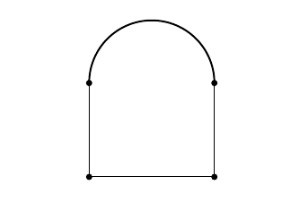
\includegraphics[scale = 1]{image5.PNG}
			\caption{Convex body with a face which is not exposed.}
		\end{center}
	\end{figure}
	
\end{remark}

\subsection{Polytopes and simple strongly isomorphic polytopes }

In this section, we define a subclass of convex bodies which are combinatorial in nature and allow us to approximate general convex bodies. We call a convex body $P \subseteq \RR^n$ a \textbf{polytope} if it can be written as the convex hull of a finite number of points. 

\begin{prop}[Properties of Polytopes]
	Let $P \subseteq \RR^n$ be an arbitrary polytope. Then, $P$ satisfies the following properties: 
	\begin{enumerate}[label = (\alph*)]
		\item The exposed faces of $P$ are exactly the faces of $P$. Moreover, $P$ has a finite number of faces. 
		\item Let $F_1, \ldots, F_k$ be the facets of $P$ with normal vectors $u_1, \ldots, u_k$. Then 
		\[
			P = \bigcap_{i = 1}^k H_{u_i, h_P(u_i)}^-
		\]
		In particular, the numbers $h_P(u_1), \ldots, h_P(u_k)$ determine $P$ uniquely. 

		\item The face poset $\mathcal{F}(P)$ of $P$ is a graded lattice which is graded by dimension. It satisfies the \textbf{Jordan-Dedekind chain condition}. In other words, if we have a face $F^j \in \mathcal{F}_j(P)$ and a face $F^k \in \mathcal{F}_k(P)$ satisfying $F^j \subset F^k$, then there are faces $F^i \in \mathcal{F}_i(P)$ for $j+1 \leq i \leq k-1$ such that 
		\[
			F^j \subset F^{j+1} \subset \ldots \subset F^{k-1} \subset F^k.
		\]
	\end{enumerate}
\end{prop}

\begin{proof}
	These properties follow from Corollary 2.4.2, Theorem 2.4.3, Corollary 2.4.4, and Corollary 2.4.8 in \cite{schneider_2013}. 
\end{proof}
\begin{example}[Order Polytope]
	We give an example of a polytope associated with a poset. Let $(P, \leq)$ be a finite poset. Now, consider the Euclidean space $\RR^P$ where the coordinates are indexed by the elements of $P$. Every vetor $v \in \RR^P$ can be written in the form $v = \sum_{\omega \in P} v_\omega \cdot e_\omega$ where $\{e_\omega\}_{\omega \in P}$ is a chosen orthonormal basis for $\RR^P$. Then, we can define the \textbf{order polytope} of $P$ to be the polytope given by
	\[
		\mcO_P := \{x \in [0, 1]^P : x_{i} \geq x_{j} \text{ whenever } i \geq j \text{ in } P\}.
	\]
	This polytope will come into play in Chapter~\ref{log-concavity-results} when we cover some log-concavity results on posets using Theorem~\ref{AF-inequality}. Given any bijection $l : P \to [n]$, we can define the \textbf{linear extension simplex}
	\[
		\Delta_l := \{x \in [0, 1]^n : 0 \leq x_{l^{-1}(1)} \leq \ldots \leq x_{l^{-1}}(n) \leq 1\}.
	\]
	Note that if $e(P)$ is the set of linear extensions of $P$, we can triangulate the order polytope as 
	\[
		\mcO_P := \bigsqcup_{l \in e(P)} \Delta_l
	\]
	where in the union, the simplicies are disjoint except possibly on the boundary. In particular, this implies that 
	\begin{equation} \label{volume-of-order-polytope}
		\Vol_n \left (\mathcal{O}_P \right ) = \frac{e(P)}{n!}
	\end{equation}
	and also the more familiar formula $\Vol_n (\Delta) = 1/n!$ where we apply Equation~\ref{volume-of-order-polytope} on the poset on $n$ elements and no comparability relations. Geometrically, we are partitioning the unit hypercube into $n!$ simplices. 
\end{example}

\begin{example}[Matroid Polytope]

\end{example}

\begin{example}[Zonotope] \label{zonotope-example}
	In this example, we give a generalization of parallelograms in planar geometry. For any vectors $v_1, \ldots, v_l \in \RR^n$, we can define the \textbf{zonotope} generated by these vectors by 
	\[
		Z(v_1, \ldots, v_l) := [0, v_1] + \ldots + [0, v_l] = \left \{ \sum_{i = 1}^l \lambda_i v_i : \lambda_i \in [0, 1] \right \}.
	\]
\end{example}
We call a polytope $P \subseteq \RR^n$ \textbf{simple} if $\text{int} (P) \neq \emptyset$ and each of its vertices is contained in exactly $n$ facets. We say two polytopes $P_1, P_2$ are called \textbf{strongly isomorphic} if $\dim F_{P_1}(u) = \dim F_{P_2}(u)$ for all $u \in \RR^n \backslash \{0\}$. Strong isomorphisms is a strong equivalence relation between polytopes which implies that two polytopes have isomorphic face lattices with corresponding faces being parallel to each other. To illustrate the strength of this equivalence relation, it can be shown that given two strongly isomorphic polytopes, the corresponding faces are also strongly isomorphic. 

\begin{lem}[Lemma 2.4.10 in \cite{schneider_2013}] \label{family-of-strongly-isomorphic}
	If $P_1, P_2$ are strongly isomorphic polytopes, then for each $u \in \RR^n \backslash \{0\}$, the faces $F_{P_1}(u)$ and $F_{P_2}(u)$ are strongly isomorphic. 
\end{lem}
\begin{proof}
	See Lemma 2.4.10 in \cite{schneider_2013}. 
\end{proof}

Given any two polytopes, it is not difficult to construct an infinite family of polytopes which are in the same strong isomorphism class. Indeed, any pair of positively-weighted Minkowski sums of two polytopes are strongly isomorphic. 

\begin{prop}[Corollary 2.4.12 in \cite{schneider_2013}] \label{families-of-strongly-isomorphic}
	If $P_1, P_2 \subseteq \RR^n$ are polytopes which are strongly isomorphic, then $\lambda_1 P_1 + \lambda_2 P_2$ with $\lambda_1, \lambda_2 > 0$ are strongly isomorphic. If $P_1, P_2$ were strongly isomorphic to begin with, then the polytopes $\lambda_1 P_1 + \lambda_2 P_2$ with $\lambda_1, \lambda_2 \geq 0$ and $\lambda_1 + \lambda_2 > 0$ are strongly isomorphic. 
\end{prop}

\begin{proof}
	See Corollary 2.4.12 in \cite{schneider_2013}.
\end{proof}

Any polytope is general is determined by its facet normals and its support values at these facet normals. Given an strong isomorphism class of polytopes $\alpha$ with facet normals $\mathcal{U}$, since all of the polytopes share the same collection of facet normals the polytopes in this isomorphism class are \textit{uniquely} determined by their support values at each of the facet normals. In other words, there is injective map $h : \alpha \to \RR^\mathcal{U}$ from the strong isomorphism class to the finite-dimensional vector space $\RR^{\mathcal{U}}$ defined by 
\[
	h_P := h(P) = \left ( H^-_{u, h_P(u)}\right )_{u \in \mathcal{U}}
\]
For a polytope $P \in \alpha$, we call $h_P := h(P)$ the \textbf{support vector} of $P$. he map $h$ is not surjective. Indeed, there are some choices of the support values at the facet normals which do not give a polytope in the same isomorphism class. For example, by taking all of the coordinates of $x \in \RR^{\mathcal{U}}$ sufficiently negative, the corresponding polytope with those support values could be empty. The structure of simple strongly isomorphism polytopes is robust: under small perturbations simple polytope remains in its strong isomorphism class. As a corollary, we prove that any vector in $\RR^{\mathcal{U}}$ can be written as a scalar multiple of the difference of two support vectors. 

\begin{lem} \label{perturbation-SSI}
	Let $P$ be a simple $n$-polytope with facet normals $\mathcal{U}$. Then, there is a number $\beta > 0$ such that every polytope of the form 
	\[
		P' := \bigcap_{u \in \mathcal{U}} H_{u, h_P(u) + \alpha_u}^-
	\]
	with $|\alpha_u| \leq \beta$ is simple and strong isomorphic to $P$. 
\end{lem}

\begin{cor} [Lemma 5.1 in \cite{bochner}]\label{difference-of-support-vectors}
	Let $\alpha$ be the strong isomorphic class of a simple polytope $P$ with facet normals $\mathcal{U}$. For any $x \in \RR^{\mathcal{U}}$ there are $a > 0$ and $Q \in \alpha$ such that $x = a (h_Q - h_P)$. 
\end{cor}

\begin{proof}
	From Lemma~\ref{perturbation-SSI} there exists $a^{-1} > 0$ sufficiently small and $Q \in \alpha$ such that $h_Q = a^{-1}(x + h_P)$. By rearranging the equation, we get $x = a(h_Q - h_P)$. 
\end{proof}

We will be interested in approximating a set of convex bodies by polytopes which are simple and strongly isomorphic. To make sense of approximation of polytopes, we will equip the space of convex bodies with a metric.

\subsection{Hausdorff metric on convex bodies}

In this subsection, we equip the space of convex bodies $\mathsf{K}^n$ with the Hausdorff metric $\delta$. We define the \textbf{Hausdorff metric} of $K, L \in \mathsf{K}^n$ as 

Since convex sets are closed, it is Lebesgue measurable. Hence, it has a well-defined volume which we define as 
\begin{align*}
	\delta (K, L) & = \max \left \{ \sup_{x \in K} \inf_{y \in L} |x-y|, \sup_{y \in L} \inf_{x \in K} |x-y|\right \} \\
	& = \inf \{\varepsilon \geq 0 : K \subseteq L + \varepsilon B^n, L \subseteq K + \varepsilon B^n\} \\
	& = \norm{h_K - h_L}_\infty.
\end{align*}
For a proof of the equivalence of these three descriptions, we direct the reader to Theorem 3.2 in \cite{Hug2020-ue}. In Proposition~\ref{convex-body-is-metric-space}, we prove that $\delta$ is a metric on the space of convex bodies. In Theorem~\ref{approximation-SSI}, we prove that any set of convex bodies can be approximated by simple polytopes such that each simple polytope in the approximation are strongly isomorphic. 

\begin{prop} \label{convex-body-is-metric-space}
	The ordered pair $(\mathsf{K}^n, \delta)$ is a metric space. 
\end{prop}

\begin{proof}
	For $K, L, M \in \mathsf{K}^n$, we have 
	\[
		\delta(K, M) = \norm{h_K - h_M}_\infty \leq \norm{h_K - h_L}_\infty + \norm{h_L - h_M}_\infty = \delta(K, L) + \delta(L, M). 
	\]
	It is clear that $\delta (K, L) = \delta (L, K)$. Finally, we have $\delta(K, L) = 0$ if and only if $\norm{h_K - h_L}_\infty = 0$. Since $h_K$ and $h_L$ are continuous function, this is true if and only if $h_K = h_L$. Since $K$ and $L$ are the intersections of their support hyperplanes, this implies that $K = L$. This suffices for the proof. 
\end{proof}

\begin{thm}[Theorem 2.4.15 in \cite{schneider_2013}] \label{approximation-SSI}
	Let $K_1, \ldots, K_m \in \mathsf{K}^n$ be convex bodies. To every $\varepsilon > 0$, there are simple strongly isomorphic polytopes $P_1, \ldots, P_m$ such that $\delta (K_i, P_i) < \varepsilon$ for $i = 1, \ldots, m$.
\end{thm}

\begin{proof}
	See Theorem 2.4.15 in \cite{schneider_2013}. 
\end{proof}

In order for approximations to be useful, we need functions on $(\mathsf{K}^n, \delta)$ which are continuous. Since convex bodies are compact, they are also Lebesgue and Borel measurable. Thus, there is a well-defined function $\Vol_n : \mathsf{K}^n \to \RR_{\geq 0}$ defined by
\[
	\Vol_n (K) := \int_{x \in \RR^n} \1_K(x) \, d \lambda(x)
\]
where $\lambda$ is the Lebesgue measure on $\RR^n$. Then $\Vol_n(\cdot)$ is a continuous function on $(\mathsf{K}^n, \delta)$. For a proof of this fact, see Theorem 1.8.20 in \cite{schneider_2013}. For another example of a continuous map, consider the projection map $p : \mathsf{K}^n \times \RR^n \to \RR^n$ which maps $(K, x) \mapsto p(K, x)$ where $p(K, x)$ is the projection of $x$ onto $K$. For the proof that this map is continuous, see Section 1.8 in \cite{schneider_2013}. Finally, the map induced by the Minkowski sum $\mathsf{K}^n \times \mathsf{K}^n \to \mathsf{K}^n$ is continuous. 


\subsection{Mixed Volumes}

Recall that in the setting of mixed discriminants, for $n \times n$ matrices $A_1, \ldots, A_m$ we had the identity
\begin{equation} \label{ye-old}
	\det (\lambda_1 A_1 + \ldots + \lambda_m A_m) = \sum_{i_1, \ldots, i_n = 1}^m \lambda_{i_1} \ldots \lambda_{i_n} \cdot \mathsf{D}(A_{i_1}, \ldots, A_{i_n})
\end{equation}
where the multilinear form $\mathsf{D}$ was the mixed discriminant. In this subsection, we aim to achieve a similar expression in the world of convex bodies. That is, for convex bodies $K_1, \ldots, K_m \subseteq \RR^n$, we want to expand $\Vol_n(\lambda_1 K_1 + \ldots + \lambda_m K_m)$ as a homogeneous polynomial. 
\begin{example}
	Let $K \subseteq \RR^2$ be a polygon and $L \subseteq \RR^2$ be the unit disc. Then by drawing $\lambda K + \mu L$ on the plane, we can compute 
	\[
		\Vol_2 (\lambda K + \mu L) = \lambda^2 \Vol_2(K) + \lambda \mu \cdot \mathsf{perimeter}(K) + \mu^2 \Vol_2(L). 
	\]
	This provides some evidence of a expansion of the form Equation~\ref{ye-old} since the coefficients seem to encode geometric information about the convex bodies $K$ and $L$. 
\end{example}

We first define mixed volumes in for polytopes and then extend this continuously to the space of convex bodies. 

\begin{defn}
	For $n \geq 2$, let $P_1, \ldots, P_n \subseteq \RR^n$ be polytopes and let $\mathcal{U}$ be the set of unit facet normals of $P_1 + \ldots + P_{n-1}$. We define their mixed volume $\mathsf{V}_n(P_1, \ldots, P_n)$ inductively by 
	\[
		\mathsf{V}_n(P_1, \ldots, P_n) = \frac{1}{n} \sum_{u \in \mathcal{U}} h_{P_n}(u) \cdot \mathsf{V}_{n-1} (F_{P_1}(u), \ldots, F_{P_{n-1}}(u)).
	\]
	On the right hand side of the equation though $F_{P_1}(u), \ldots, F_{P_{n-1}}(u)$ are in $\RR^n$, since they are in parallel hyperplanes we can consider them as subsets of $\RR^{n-1}$ by projecting them orthogonally on the same hyperplane isomorphic to $\RR^{n-1}$. Thus, the mixed volume $\mathsf{V}_{n-1}(F_{P_1}(u), \ldots, F_{P_{n-1}}(u))$ is well-defined. For $n = 1$, we define $V_1 ([a, b]) = b-a$. 
\end{defn}

\begin{thm}[Theorem 3.7 in \cite{Hug2020-ue}] \label{mixed-volume-polynomial-expansion}
	For polytopes $P_1, \ldots, P_m \subseteq \RR^n$ be polytopes. Then, we have 
	\[
		\Vol_n(\lambda_1 P_1 + \ldots + \lambda_m P_m) = \sum_{i_1, \ldots, i_n = 1}^m \lambda_{i_1} \ldots \lambda_{i_n} \cdot \mathsf{V}_n (P_{i_1}, \ldots, P_{i_n}).
	\]
\end{thm}

\begin{proof}
	It suffices to prove the equality when $\lambda_1, \ldots, \lambda_m > 0$ since the general equality will follow from continuity. In this case, Proposition~\ref{families-of-strongly-isomorphic} implies that $\lambda_1 P_1 + \ldots + \lambda_m P_m$ and $P_1 + \ldots + P_m$ are strongly isomorphic. Thus the set of facet normals $\mathcal{U}$ are the same for both of these polytopes. We can compute 
	\begin{align*}
		\Vol_n (\lambda_1 P_1 + \ldots + \lambda_m P_m) & = \frac{1}{n} \sum_{u \in \mathcal{U}} h_{\lambda_1 P_1 + \ldots + \lambda_m P_m}(u) \cdot \Vol_{n-1} \left ( F_{\lambda_1 P_1 + \ldots + \lambda_m P_m} (u) \right ) \\
		& = \frac{1}{n} \sum_{u \in \mathcal{U}} \sum_{i = 1}^n \lambda_i h_{P_i}(u) \cdot \Vol_{n-1} \left ( \sum_{i = 1}^m \lambda_i F_{P_i}(u) \right ) \\
		& = \frac{1}{n} \sum_{u \in \mathcal{U}} \sum_{i_1, \ldots, i_n = 1}^m \lambda_{i_1} \ldots \lambda_{i_n} \cdot h_{P_{i_n}}(u) \cdot \mathsf{V}_{n-1} \left (F_{P_{i_1}}(u), \ldots, F_{P_{i_{n-1}}}(u) \right ) \\
		& = \sum_{i_1, \ldots, i_n = 1}^m \lambda_{i_1} \ldots \lambda_{i_n} \sum_{u \in \mathcal{U}} \frac{1}{n} h_{P_{i_n}}(u) \cdot \mathsf{V}_{n-1} \left (F_{P_{i_1}}(u), \ldots, F_{P_{i_{n-1}}}(u) \right ) \\
		& = \sum_{i_1, \ldots, i_n = 1}^m \lambda_{i_1} \ldots \lambda_{i_n} \cdot \mathsf{V}_n \left (F_{P_{i_1}}(u), \ldots, F_{P_{i_{n}}}(u) \right ). 
	\end{align*}
	This suffices for the proof. 
\end{proof}

A apriori it is not clear that the mixed volume from how we defined it is symmetric in its arguments. To prove that it is indeed symmetric in its arguments, we present the proof of Theorem~\ref{inversion-formula} from \cite{schneider_2013}. This result will not only prove that the mixed volume is symmetric, but it will also prove that we can extend the mixed volume to all convex bodies rather than just polytopes. 

\begin{thm}[Inversion Formula, Lemma 5.1.4 in \cite{schneider_2013}] \label{inversion-formula}
	For polytopes $P_1, \ldots, P_n \subseteq \RR^n$, we have
	\begin{align*}
		\mathsf{V}_n(P_1, \ldots, P_n) & = \frac{1}{n!} \sum_{k = 1}^n (-1)^{n+k} \sum_{1 \leq r_1 < \ldots < r_k \leq n} \Vol_n (P_{r_1} + \ldots + P_{r_k}) \\
		& = \frac{1}{n!} \sum_{I \subseteq [n]} (-1)^{n - |I|} \Vol_n \left ( \sum_{i \in I} P_i \right ).
	\end{align*}
\end{thm}

\begin{proof}
	We present the proof in \cite{schneider_2013} for the sake of completeness. We can define the function $f : \RR^n \to \RR$ defined by 
	\[
		f(\lambda_1, \ldots, \lambda_n) := \frac{1}{n!} \sum_{k = 1}^n (-1)^{n+k} \sum_{1 \leq r_1 < \ldots < r_k \leq n} \Vol_n(\lambda_{r_1} P_{r_1} + \ldots+ \lambda_{r_k} P_{r_k}).
	\]
	From Theorem~\ref{mixed-volume-polynomial-expansion}, we get that $f$ is either $0$ or a homogeneous polynomial of degree $n$. If we let $\lambda_1 = 0$, then we have
	\begin{align*}
		n! (-1)^n f(0, \lambda_2, \ldots, \lambda_n) & := S_1 + \sum_{k = 2}^n S_k
	\end{align*}
	where we define $S_1 = - \sum_{2 \leq r_1 \leq n} \Vol_n (\lambda_{r_1} P_{r_1})$ and for $k \geq 2$ we define
	\begin{align*}
		S_k & = \sum_{k = 1}^n (-1)^k \left ( \sum_{2 \leq r_2 < \ldots < r_k \leq n} \Vol_n(\lambda_{r_2} P_{r_2} + \ldots + \lambda_{r_k} P_{r_k}) + \sum_{2 \leq r_1 < \ldots < r_k \leq n} \Vol_n (\lambda_{r_1} P_{r_1} + \ldots + \lambda_{r_k} P_{r_k})\right ).
	\end{align*}
	Note that this is a telescoping sum and $f(0, \lambda_2, \ldots, \lambda_n) = 0$. By symmetry, we know that $f$ is a scalar multiple of $\lambda_1 \ldots \lambda_n$. The only term in $f$ which contributes $\lambda_1 \ldots \lambda_n$ is in $\Vol_n (\sum_{i = 1}^n \lambda_i P_i)$. Thus, we have that 
	\[
		f(\lambda_1, \ldots, \lambda_n) = \lambda_1 \ldots \lambda_n \cdot \mathsf{V}_n (P_1, \ldots, P_n).
	\]
	By substituting $\lambda_1 = \ldots = \lambda_n = 1$, this completes the proof. 
\end{proof}

For an example of the inversion formula, we will compute the mixed volume of a collection of line segments.

\begin{example}\label{mixed-volume-of-line-segments}
	Let $v_1, \ldots, v_n \in \RR^n$ be vectors. Then, from the inversion formula, we have that 
	\begin{align*}
		\mathsf{V}_n([0, v_1], \ldots, [0, v_n]) = \frac{1}{n!} \Vol_n ([0, v_1] + \ldots + [0, v_n])
	\end{align*}
	where the other summands are zero since they are contained in lower dimensional affine spaces. Let $T : \RR^n \to \RR^n$ be the linear map which sends $Te_i = v_i$ for $1 \leq i \leq n$. Then, 
	\[
		[0, v_1] + \ldots + [0, v_n] = T ([0, 1]^n).
	\]
	This gives us the identity 
	\[
		\mathsf{V}_n([0, v_1], \ldots, [0, v_n]) = \frac{1}{n!} \Vol_n(T([0, 1]^n)) = \frac{1}{n!} |\text{Det}(v_1, \ldots, v_n)|.
	\]
\end{example}

Since the volume functional is continuous on the space of convex bodies equipped with Hausdorff distance, we can extend the definition of mixed volumes to general convex bodies via continuity. 

\begin{defn}
	Let $K_1, \ldots, K_n \subseteq \RR^n$ be convex bodies. Then, we define the \textbf{mixed volume} of $K_1, \ldots, K_n$ as  
	\[
		\mathsf{V}_{n}(K_1, \ldots, K_n) := \frac{1}{n!} \sum_{I \subseteq [n]} (-1)^{n- |I|} \Vol_n \left ( \sum_{i \in I} P_i \right ).
	\]
\end{defn}

By defining the mixed volume in this way, we immediately get from Theorem~\ref{inversion-formula} that if $P^{(i)}_k$ for $1 \leq i \leq n$ is a sequence of polytopes such that $P_1^{(k)} \longrightarrow K_i$ as $k \to \infty$, then 
\[
	\mathsf{V}_n(K_1, \ldots, K_n) = \lim_{k \to \infty} \mathsf{V}_n (P_1^{(k)}, \ldots, P_n^{(k)}).
\] 
This is because both $\Vol_n$ and Minkowski sums are continuous on the space of convex bodies. Furthermore, continuity lets us extend Theorem~\ref{mixed-volume-polynomial-expansion} to general convex bodies. 
\begin{thm} \label{mixed-volume-polynomial-expansion-FINAL}
	Let $K_1, \ldots, K_m \subseteq \RR^n$ be convex bodies. Then, we have 
	\[
		\Vol_n (\lambda_1 K_1 + \ldots + \lambda_m K_m) = \sum_{i_1 , \ldots , i_n = 1}^m \lambda_{i_1} \ldots \lambda_{i_n} \cdot \mathsf{V}_n (K_{i_1}, \ldots, K_{i_n}).
	\]
\end{thm}

\begin{proof}
	For $1 \leq i \leq n$, let $P_i^{(k)}$ for $k \geq 1$ be a sequence of polytopes converging to $K_i$ in Hausdorff distance. Then, we have 
	\begin{align*}
		\Vol_n \left ( \sum_{i = 1}^n \lambda_i K_i \right ) & = \lim_{k \to \infty} \Vol_n \left ( \sum_{i = 1}^n \lambda_i P_i^{(k)} \right ) \\
		& = \lim_{k \to \infty} \sum_{i_1 , \ldots , i_n = 1}^m \lambda_{i_1} \ldots \lambda_{i_n} \cdot \mathsf{V}_n (P_{i_1}^{(k)}, \ldots, P_{i_n}^{(k)}) \\
		& = \sum_{i_1 , \ldots , i_n = 1}^m \lambda_{i_1} \ldots \lambda_{i_n} \cdot \lim_{k \to \infty} \mathsf{V}_n (P_{i_1}^{(k)}, \ldots, P_{i_n}^{(k)}) \\
		& = \sum_{i_1 , \ldots , i_n = 1}^m \lambda_{i_1} \ldots \lambda_{i_n} \cdot \mathsf{V}_n (K_{i_1}, \ldots, K_{i_n}).
	\end{align*}
	This suffices for the proof. 
\end{proof}

\begin{example}[Volume of a Zonotope] \label{example-volume-of-a-zonotope}
	From Theorem~\ref{mixed-volume-polynomial-expansion-FINAL}, we can compute the volume of a zonotope. Let $v_1, \ldots, v_l \in \RR^n$ be vectors. Then, we have that 
	\begin{align*}
		\Vol_n (Z(v_1, \ldots, v_l)) & = \Vol_n \left ( \sum_{i = 1}^l [0, v_i] \right ) \\
		& = \sum_{i_1, \ldots, i_n = 1}^l \mathsf{V}_n ([0, v_{i_1}], \ldots, [0, v_{i_n}]) \\
		& = \sum_{i_1, \ldots, i_n = 1}^l \frac{1}{n!} |\text{Det}(v_{i_1}, \ldots, v_{i_n}) | \\
		& = \sum_{1 \leq i_1 < \ldots < i_n \leq l} |\text{Det}(v_{i_1}, \ldots, v_{i_n})|
	\end{align*}
	where the equality in the third line follows from the computation in Example~\ref{mixed-volume-of-line-segments}. 
\end{example}

We now define the notion of mixed area measures which is measure-theoretic interpretation of the mixed volumes. This notion will become essential when considering the equality cases of the Alexandrov-Fenchel inequality. Our treatment of mixed area measures is inspired by Chapter 4 in \cite{Hug2020-ue}. Recall that for polytopes $P_1, \ldots, P_n$, we define the mixed volume as 
\[
	\mathsf{V}_n (P_1, \ldots, P_n) = \frac{1}{n} \sum_{u \in \mathbb{S}^{n-1}} h_{P_n}(u) \cdot \mathsf{V}_{n-1}(F_{P_1}(u), \ldots, F_{P_{n-1}}(u))
\]
where the sum is well-defined because the number of facet normals. Outside of these facet normals, the mixed volume inside the sum vanishes. For any convex body $K \subseteq \RR^n$ which is not necessarily polytopal, we can take a sequence $P_n^k \to K$ as $k \to \infty$ to get the identity
\[
	\mathsf{V}_n(P_1, \ldots, P_{n-1}, K) = \frac{1}{n} \sum_{u \in \mathbb{S}^{n-1}} h_{K_n}(u) \cdot \mathsf{V}_{n-1}(F_{P_1}(u), \ldots, F_{P_{n-1}}(u)).
\]
Measure-theoretically, we can define a measure on the unit sphere defined by
\[
	S_{P_1, \ldots, P_{n-1}} := \sum_{u \in \mathbb{S}^{n-1}} \mathsf{V}_{n-1}(F_{P_1}(u), \ldots, F_{P_{n-1}}(u)) \cdot \delta_u
\]
where $\delta_u$ is the dirac delta measure at $u$. Then, we have 
\[
	\mathsf{V}_n(P_1, \ldots, P_{n-1}, K) = \frac{1}{n} \int_{\mathbb{S}^{n-1}} h_{K}(u) \, S_{P_1, \ldots, P_{n-1}}(du).
\]
We have defined this measure in the case where the first $n-1$ convex bodies in the mixed volume are polytopes. From the Riesz representation theorem, it can be shown that such a measure exists for general convex bodies (see Theorem 4.1 in \cite{Hug2020-ue} and Theorem 2.14 in \cite{rudin}).

\begin{thm} [Theorem 4.1 in \cite{Hug2020-ue}]
	For convex bodies $K_1, \ldots, K_{n-1} \subseteq \RR^n$, there exists a uniquely determined finite Borel measure $S_{K_1, \ldots, K_{n-1}}$ on $\mathbb{S}^{n-1}$ such that 
	\[
		\mathsf{V}(K_1, \ldots, K_{n-1}, K) = \frac{1}{n} \int_{\mathbb{S}^{n-1}} h_K(u) \, S_{K_1, \ldots, K_{n-1}} (du)
	\]
	for all convex bodies $K \subseteq \RR^n$. 
\end{thm}

\begin{defn}
	For convex bodies $K_1, \ldots, K_{n-1} \subseteq \RR^n$, we call the measure $S_{K_1, \ldots, K_{n-1}}$ the \textbf{mixed area measure} associated with $(K_1, \ldots, K_{n-1})$. 
\end{defn}

\subsection{Positivity and Normal Directions}

In this section, we discuss when the mixed volume of a collection of convex bodies is positive. The necessary and sufficient conditions for positivity are collected in Lemma~\ref{positivity-of-mixed-volumes}. 

\begin{lem}[Lemma 2.2 in \cite{shenfeld2022extremals}] \label{positivity-of-mixed-volumes}
	For conex bodies $C_1, \ldots, C_n \subseteq \RR^n$, the following two conditions are equivalent.
	\begin{enumerate}[label = (\alph*)]
		\item $\mathsf{V}_n (C_1, \ldots, C_n) > 0$. 
		\item There are segments $I_i \subseteq C_i$, $i \in [n]$ with linearly independent directions. 
		\item $\dim (C_{i_1} + \ldots + C_{i_k}) \geq k$ for all $k \in [n]$, $1 \leq i_1 < \ldots < i_k \leq n$. 
	\end{enumerate}
\end{lem}

Next, we provide necessary and sufficient conditions for a vector to be in the support of the mixed area measure $S_{B, P_1, \ldots, P_{n-2}}$ where $P_1, \ldots, P_{n-2}$ are polytopes. The terminology used in Definition~\ref{extreme-normal-directions} was introduced in Lemma 2.3 of \cite{shenfeld2022extremals}. 

\begin{defn}[Lemma 2.3 in \cite{shenfeld2022extremals}] \label{extreme-normal-directions}
	For $P_1, \ldots, P_{n-2} \subseteq \RR^n$ convex polytopes and $u \in \mathbb{S}^{n-1}$. We call $u$ a $(B, P_1, \ldots, P_{n-2})$-extreme \textbf{normal direction} if and only if at least one of the following three equivalent conditions hold:
	\begin{enumerate}[label = (\alph*)]
		\item $u \in \supp S_{B, P_1, \ldots, P_{n-2}}$. 
		\item There are segments $I_i \subseteq F (P_i, u)$, $i \in [n-2]$ with linearly independent directions. 
		\item $\dim(F(P_{i_1}, u) + \ldots + F(P_{i_k}, u)) \geq k$ for all $k \geq [n-2]$, $1 \leq i_1 < \ldots < i_k \leq n-2$. 
	\end{enumerate}
\end{defn}

The fact that (a)-(c) are equivalent in Definition~\ref{extreme-normal-directions} is exactly the content of Lemma 2.3 in \cite{shenfeld2022extremals}. 

\chapter{Mechanisms for Log-concavity}


\section{Log-Concavity and Ultra Log-Concavity}

\begin{defn}

\end{defn}
	
\begin{example}
	The sequence of binomial coefficients $\binom{n}{k}$ forms a log-concave sequence. 
\end{example}
(Many sequences in combinatorics are proven to be log-concave ... give examples: Read's conjecture, Mason's Conjecture, etc. )

\begin{example}[The Mason Conjectures]
	Let $M$ be a matroid of rank $r$. For $0 \leq i \leq r$, let $I_i$ denote the number of independent sets of $M$ with $i$ elements. Then there are three conjectures of increasing strength related to the log-concavity of this sequence. 
	\begin{enumerate}
		\item (Mason Conjecture) $I_k^2 \geq I_{k-1} I_{k+1}$. 
		\item (Strong Mason Conjecture) $I_k^2 \geq \left (1 + \frac{1}{k} \right ) I_{k-1} I_{k+1}$. 
		\item (Ultra-Strong Mason Conjecture) $I_k^2 \geq \left (1 + \frac{1}{k} \right ) \left (1 + \frac{1}{n-k} \right ) I_{k-1} I_{k+1}$. 
	\end{enumerate}
	The Mason conjecture says that the sequence $I_i$ is log-concave while the ultra-strong Mason conjecture states that the sequence $I_i$ is ultra-log-concave. All three of these conjectures have been proven. In \cite{AHK}, Karim Adiprasito, June Huh, and Eric Katz proved the Mason conjecture by developing a hodge theory of matroids. Later, the strong Mason conjecture was proven by June Huh, Benjamin Schro"ter, and Botong Wang in \cite{correlation-bounds} and Nima Anari, Kuikui Liu, Shayan Oveis Gharan, and Cynthia Vinzant in \cite{anari2018logconcave} independently. 
\end{example}

\section{Cauchy's Interlacing Theorem}

Given an $n \times n$ matrix $A$, we call a submatrix $B$ a \textbf{principal submatrix} if it is obtained from $A$ by deleting some rows and the corresponding columns. When $A$ is a Hermitian matrix and $B$ is a principal submatrix of size $(n-1) \times (n-1)$, Theorem~\ref{cauchy-interlacing} gives a mechanism for controlling the eigenvalues of $B$ based on $A$. We present a short proof from \cite{fisk} of this result. For different proofs using the intermediate value theorem, Sylvester's law of inertia, and the Courant-Fischer minimax theorem, we direct the reader to the references \cite{suk}, \cite{symmetric-eigenvalue-problem}, and \cite{GoluVanl96}, respectively. 

\begin{thm}[Cauchy Interlace Theorem] \label{cauchy-interlacing}
	Let $A$ be a Hermitian matrix of order $n$, and let $B$ be a principal submatrix of $A$ of order $n-1$. If $\lambda_n \leq \lambda_{n-1} \leq \ldots \leq \lambda_2 \leq \lambda_1$ are the eigenvalues of $A$ and $\mu_n \leq \mu_{n-1} \leq \ldots \leq \mu_3 \leq \mu_2$ are the eigenvalues of $B$. Then, we have
	\[
		\lambda_n \leq \mu_n \leq \lambda_{n-1} \leq \mu_{n-1} \leq \ldots \leq \lambda_2 \leq \mu_2 \leq \lambda_1.
	\]
\end{thm}

Before proving this result, we need Theorem~\ref{interlacing-roots-of-polynomial} which is a theorem about when roots of polynomials interlace. Suppose that $f, g \RR[x]$ are real polynomials with only real roots. We say that the polynomials $f$ and $g$ \textbf{interlace} if their roots $r_1 \leq \ldots \leq r_n$ and $s_1 \leq \ldots \leq s_{n-1}$ satisfy
\[
	r_1 \leq s_1 \leq \ldots \leq r_{n-1} \leq s_{n-1} \leq r_n.
\]

\begin{thm} \label{interlacing-roots-of-polynomial}
	Let $f, g \in \RR[x]$ be polynomials with only only real roots. Suppose that $\deg (f) = n$ and $\deg (g) = n-1$. Then, $f$ and $g$ interlace if and only if the linear combinations $f + \alpha g$ have all real roots for all $\alpha \in \RR$. 
\end{thm} 
\begin{proof}
	See Theorem 6.3.8 in \cite{rahman}.
\end{proof}

\begin{proof}[Proof of Theorem~\ref{cauchy-interlacing}]
	We follow the proof in \cite{fisk}. Without loss of generality, we can decompose 
	\[
		A = \begin{bmatrix}
			B & v \\
			v^T & c
		\end{bmatrix}
	\]
	where $v \in \RR^{(n-1) \times 1}$ and $c \in \RR$. Consider the polynomials $f(x) := \det (A - xI)$ and $g(x) := \det (B - xI)$. Note that the roots of $f$ and $g$ are all real and are exactly the eigenvalues of $A$ and $B$, respectively. For any $\alpha \in \RR$, we have
	\begin{align*}
		f(x) + \alpha g(x) & = \det\begin{bmatrix}
			B-xI & v \\
			v^T & d-x
		\end{bmatrix} + \alpha \det \begin{bmatrix}
			B-xI & v \\
			0 & 1
		\end{bmatrix} \\
		& = \det\begin{bmatrix}
			B-xI & v \\
			v^T & d-x
		\end{bmatrix} + \det \begin{bmatrix}
			B-xI & v \\
			0 & \alpha
		\end{bmatrix} \\
		& = \det \begin{bmatrix}
			B-xI & v \\
			v^T & d+\alpha - x
		\end{bmatrix}.
	\end{align*}
	Thus $f + \alpha g$ is the characteristic polynomial of a Hermitian matrix and has real roots. From Theorem~\ref{interlacing-roots-of-polynomial}, the proof is complete. 
\end{proof}

\begin{cor}
	Let $M$ be a $n \times n$ matrix with exactly one positive eigenvalue. If $A$ is a principal matrix $A$ of size $2 \times 2$ such that there exists $v \in \RR^2$ with $v^T A v > 0$, then $\det (A) \leq 0$. 
\end{cor}

\begin{proof}
	From Theorem~\ref{cauchy-interlacing}, the matrix $A$ has at most one positive eigenvalue. Since $v^T A v > 0$, we know that $A$ has exactly one positive eigenvalue. The other eigenvalue must be at most $0$. Hence, we have $\det (A) \leq 0$. This suffices for the proof. 
\end{proof}

\section{Alexandrov's Inequality for Mixed Discriminants}

In this section we introduce a fundamental inequality given in Theorem~\ref{A-Inequality-MIXED-DISCRIMINANT} in the theory of mixed discriminants. This inequality is similar to the inequality for mixed volumes of convex bodies given in Theorem~\ref{AF-inequality}. We first give a generalization of this inequality to the larger class of objects called \textbf{hyperbolic polynomials}. For an introduction to the theory of hyperbolic polynomials, we refer the reader to \cite{schneider_2013} and \cite{hyperbolic-polynomials}. We call a homogeneous polynomial $p \in \RR[x_1, \ldots, x_n]$ \textbf{hyperbolic in direction} $v$ for $v \in \RR^n$ if and only if $p(v) > 0$ and for each $x \in \RR^n$, the univariate polynomial $p(x + tv)$ when considered a polynomial in $t$ has only real roots. If $p$ is hyperbolic in direction $v \in \RR^n$ then we can define the hyperbolicity cone $\mathcal{H} (p)$ as the set of directions for which $p$ is hyperbolic. 

\begin{thm}[Theorem 5.5.3 in \cite{schneider_2013}]
	Let $p$ be a hyperbolic homogeneous polynomial of degree $k \geq 1$ on $\RR^n$, and let $\tilde{p}$ be its polarization. Let $y, x_2, \ldots, x_k \in \mathcal{H}(p)$, $x \in \overline{\mathcal{H}(p)}$, and $z \in \RR^n$. Then 
	\[
		\widetilde{p}(y, z, x_3, \ldots, x_k)^2 \geq \widetilde{p}(y, y, x_3, \ldots, x_k) \widetilde{p} (z, z, x_3, \ldots, x_k).
	\]
\end{thm}

\begin{proof}
	See Theorem 5.5.3 in \cite{schneider_2013}.
\end{proof}

\begin{thm} [Alexandrov's Inequality for Mixed Discriminants] \label{A-Inequality-MIXED-DISCRIMINANT}
	Let $A_1, \ldots, A_{n-2}$ be real symmetric positive definite $n \times n$ matrices. Let $X$ be a real symmetric positive definite $n \times n$ square matrix and let $Y$ be a real symmetric positive semidefinite $n \times n$ square matrix. Then 
	\[
		\mathsf{D}(X, Y, A_1, \ldots, A_{n-2})^2 \geq \mathsf{D}(X, X, A_1, \ldots, A_{n-2}) \cdot \mathsf{D} (Y, Y, A_1, \ldots, A_{n-2})
	\]
	where equality holds if and only if $B = \lambda A$ for a real number $\lambda$. 
\end{thm}

We present a proof of Theorem~\ref{A-Inequality-MIXED-DISCRIMINANT} given in \cite{bapat_raghavan_1997} and \cite{schneider-mixed-discriminants}. Before we begin the proof, we first need the following result from \cite{hardy1952inequalities}. 

\begin{lem} [\cite{hardy1952inequalities} and Lemma 5.3.2 in \cite{bapat_raghavan_1997}] \label{newton}
	Let $p(x) = \sum_{k = 0}^n \binom{n}{k} a_k x^k$ be a real-rooted univariate polynomial. Then, we have $a_k^2 \geq a_{k-1}a_{k+1}$ for all $1 \leq i \leq n-1$. If $a_0 \neq 0$ then equality occurs for any $i$ if and only if all the roots of $f(x)$ are equal. 
\end{lem}

\begin{proof}
	From Rolle's Theorem, if a polynomial is real-rooted, then so is all of its derivatives. It is also clear that when we reverse the coefficients of a real-rooted polynomial, then it remains real-rooted. We call the operation for reversing the coefficients \textbf{reciprocation} of the polynomial. This implies through a sequence of derivatives and reciprocations, we get the polynomial $\alpha_{i-1} + 2\alpha_i x + \alpha_{i+1} x^2$. Since we arrived at this polynomial throuhg a sequence of derivatives and reciprocations, we know that this polynomial is real-rooted. Hence, the discriminant is non-negative and $\alpha_i^2 \geq \alpha_{i-1} \alpha_{i+1}$. The equality case follows from the fact that Rolle's Theorem implies that the roots of the derivative of a real-rooted polynomial interlaces the roots of the original polynomial. 
\end{proof}

\begin{proof}[Proof of Theorem~\ref{A-Inequality-MIXED-DISCRIMINANT}]
	Let $A_1, \ldots, A_m$ be positive semi-definite $n \times n$ matrices. For $(r_1, \ldots, r_m) \in \Delta_m^{n}$ we define the term
	\[
		D(r_1, \ldots, r_m) := \mathsf{D}_n \left ( \underbrace{A_1, \ldots, A_1}_{r_1 \text{ times}}, \ldots, \underbrace{A_m, \ldots, A_m}_{r_m \text{ times}} \right ).
	\] 
	It suffices to prove that 
	\[
		D(r_1, \ldots, r_{m-2}, r_{m-1}, r_m)^2 \geq D(r_1, \ldots, r_{m-2}, r_{m-1}+1, r_m-1) \cdot D(r_1 \ldots, r_{m-2}, r_{m-1}-1, r_m+1).
	\]
	To prove this, we induct on $m$. Suppose that $m=2$. Consider the polynomial 
	\[
		\det (xA_1 + A_2) = \sum_{i = 0}^n \binom{n}{i} D(i, r-i) x^i.
	\]
	Since $A_1$ is positive definite, there is some positive definite $\Sigma_1$ such that $\Sigma_1^2 = A_1$. Thus, we have 
	\[
		\det (xA_1 + A_2) = \det (x\Sigma_1^2 + A_2) = \det (\Sigma_1)^2 \cdot \det (x + \Sigma_1^{-1} A_2 \Sigma_1^{-1}).
	\]
	Thus, the polynomial $\det (xA_1 + A_2)$ is real-rooted. From Lemma~\ref{newton}, this implies that $D(i, r-i)^2 \geq D(i-1, r-i+1) \cdot D(i+1, r-i-1)$ where equality holds whenever all of the roots are the same. In this case, we have $\Sigma_1^{-1} A_2 \Sigma_1^{-1} = \lambda I \implies A_2 = \lambda A_1$ for some $\lambda \in \RR$. This proves the base case. \\

	Now suppose that the claim is true for $m$. Consider a $m+1$-tuple $(r_1, \ldots, r_{m+1}) \in \Delta_{m+1}^n$ satisfying $r_1 + \ldots + r_{m+1} = n$. We want to prove that 
	\[
		D(r_1, \ldots, r_{m-1}, r_m, r_{m+1})^2 \geq D(r_1, \ldots, r_{m-1}, r_m - 1, r_{m+1}+1) \cdot D(r_1, \ldots, r_{m-1}, r_m+1, r_{m+1}-1).
	\]
	We can define $B_y := y A_m + A_{m+1}$ where $y$ is a real parameter. Then, we have that
	\[
		\det \left ( \sum_{i = 1}^{m-1} x_i A_i + x_m B_y \right ) = \sum_{r_1 + \ldots + r_m = n} \binom{n}{r_1, \ldots, r_m} D(r_1, \ldots, r_m) (y) \cdot x_1^{r_1} \ldots x_m^{r_m}
	\]
	where $D(r_1, \ldots, r_m)(y)$ is a polynomial in $y$ of degree $r_m$. We can also write 
	\begin{align*}
		\det \left ( \sum_{i = 1}^{m-1} x_i A_i + x_m B_y \right ) & = \det \left ( \sum_{i = 1}^{m-1} x_i A_i + x_m y A_m + x_m A_{m+1} \right ) 
	\end{align*}
	\[ = \sum_{r_1 + \ldots + r_{m+1} = n} \binom{n}{r_1, \ldots, r_{m+1}} D_{m+1}(r_1, \ldots, r_{m+1}) \cdot (x_1^{r_1} \ldots x_{m-1}^{r_{m-1}}) \cdot x_m^{r_m + r_{m+1}} \cdot y^{r_m} 
	\]
	\[
	= \sum_{r_1 + \ldots + r_{m-1} + r_m = n} \left \{ \sum_{i = 0}^{r_m} \binom{n}{r_1, \ldots, r_{m-1}, i, r_m - i} D_{m+1}(r_1, \ldots, r_{m-1}, i, r_m - i) \cdot y^i \right \} \cdot x_1^{r_1} \cdot x_m^{r_m}.
	\]
	Comparing coefficients, we have that 
	\begin{align*}
		D(r_1, \ldots, r_m)(y) & = \sum_{i = 0}^{r_m} \binom{n}{r_1, \ldots, r_{m-1}, i, r_m - i} D_{m+1}(r_1, \ldots, r_{m-1},i, r_m-i) y^i \\
		& = \binom{n}{r_1, \ldots, r_m} \sum_{i = 0}^{r_m} \binom{r_m}{i} D_{m+1}(r_1, \ldots, r_{m-1}, i, r_m - i) y^i.
	\end{align*}
	Now we show that if $A_m$ and $A_{m+1}$ are not proportional, then $D(r_1, \ldots, r_m)(y)$ is real-rooted with simple roots. If this is shown, then we are done from Lemma~\ref{newton}. Following the notation in \cite{schneider-mixed-discriminants}, for fixed $r_1 + \ldots + r_{m-2} \neq n$, we define the polynomial
	\begin{align*}
		Q_k(y) & := D_m(r_1, \ldots, r_{m-2}, s-k, k) (y) \\
		& = \mathsf{D}_m (\underbrace{A_1, \ldots, A_1}_{r_1}, \ldots, \underbrace{A_{m-2}, \ldots, A_{m-2}}_{r_{m-2}}, \underbrace{A_{m-1}, \ldots, A_{m-1}}_{s-k}, \underbrace{B_y, \ldots, B_y}_k).
	\end{align*}
	where $s = n - r_1 - \ldots - r_{m-2} = r_{m-1} + r_m$. From the inductive hypothesis, we have 
	\[
		Q_k(y)^2 \geq Q_{k-1}(y) \cdot Q_{k+1}(y)
	\] 
	where equality holds if and only if $B_y = \lambda_y A_{m-1}$ for some $\lambda_y \in \RR$. Let $y_0$ be a root of $Q_k$. If equality held at $y_0$, we would have $0 = Q_k^2(y_0) = Q_{k-1}(y_0) Q_{k+1}(y_0)$. We have $B_{y_0} = \lambda A_{m-1}$ for some $\lambda \in \RR$ from the inductive hypothesis. We have 
	\[
		y_0 A_m + A_{m+1} = \lambda A_{m-1}.
	\]
	Note that $\lambda \neq 0$ because then $A_m$ and $A_{m+1}$ would be proportional to each other. If $\lambda > 0$, then $B_{y_0}$ would be positive definite. But Corollary~\ref{final-positivity-corollary} implies that $Q_k(y_0) > 0$, which cannot happen. If $\lambda < 0$, then $B_{y_0}$ is negative definite. This implies that the sign of $Q_k(y_0)$ is $(-1)^k$ and is not zero. This also cannot happen. It must be the case that at all roots of $Q_k(y)$ there is strict inequality. \\

	Now we prove that $Q_k(y)$ has $k$ simple real roots where the roots of $Q_{k-1}(y)$ and $Q_k(y)$ are interlaced for $2 \leq k \leq s$. To prove that $Q_1(y)$ satisfies the claim, note that 
	\begin{align*}
		Q_1(y) & = D_m(r_1, \ldots, r_{m-2}, s-1, 1)(y) \\
		& = \mathsf{D}_m (\underbrace{A_1, \ldots, A_1}_{r_1}, \ldots, \underbrace{A_{m-2}, \ldots, A_{m-2}}_{r_{m-2}}, \underbrace{A_{m-1}, \ldots, A_{m-1}}_{s-1}, B_y) \\
		& = \mathsf{D}_m (A_1[r_1], \ldots, A_{m-2}[r_{m-2}], A_{m-1}[s-1], A_m) y + \mathsf{D}_m (A_1[r_1], \ldots, A_{m-2}[r_{m-2}], A_{m-1}[s-1], A_{m+1}).
	\end{align*}
	The coefficient in front of $y$ is positive from Corollary~\ref{final-positivity-corollary}. Thus the polynomial $Q_1(y)$ has $1$ simple real zero. Let $q_1 := q_1^{(1)}$ be the unique root of this polynomial. Then, from our earlier discussion, we have the strict inequality $Q_1(q_1)^2 > Q_0(q_1) \cdot Q_2(q_1)$. This implies that $Q_2(q_1) < 0$ since $Q_0(q_1) > 0$ from Corollary~\ref{final-positivity-corollary}. Since $Q_2(y)$ is a quadratic with a positive leading coefficient and $Q_2(q_1) < 0$, the intermediate value theorem implies that there exist $q_2^{(1)}$ and $q_2^{(2)}$ which are roots of $Q_2$ and $q_2^{(1)} < q_1^{(1)} < q_2^{(2)}$. Now, suppose that the roots of $Q_{k-1}$ are $q_{k-1}^{(1)}, \ldots, q_{k-1}^{(k-1)}$ and the roots of $Q_k$ are $q_k^{(1)}, \ldots, q_k^{(k)}$ satisfy 
	\[
		q_k^{(1)} < q_{k-1}^{(1)} < q_k^{(2)} < \ldots < q_k^{(k-1)} < q_{k-1}^{(k-1)} < q_k^{(k)}.
	\]
	Note that we have 
	\[
		Q_k(q_k^{(i)})^2 > Q_{k-1}(q_k^{(i)}) \cdot Q_{k+1}(q_k^{(i)}).
	\]
	From the inductive hypothesis, $Q_{k-1}(q_k^{(i)})$ alternates in sign. Thus $Q_{k+1}(q_k^{(i)})$ also alternates in sign. Thus the roots of $Q_{k+1}$ are simple, real, and interlace $Q_k$. This proves the auxiliary claim that $Q_k$ has $k$ simple real roots. \\

	This claim proves that $D_m(r_1, \ldots, r_{m-1}, k)(y)$ has $k$ simple real roots. This proves the desired inequality and also guarentees that it is strict in the case where $A_m$ and $A_{m+1}$ are not proportional. This completes the induction and suffices for the proof. 
\end{proof}


\begin{cor} \label{mixed-discriminant-log-concave-sequence}
	Let $A, B$ be $n \times n$ positive definite symmetric real matrices. For $0 \leq k \leq n$, define the mixed discriminant
	\[
		D_k := \mathsf{D} (\underbrace{A, \ldots, A}_{k \text{ times}}, \underbrace{B \ldots, B}_{n-k \text{ times}}).
	\]
	Then the sequence $D_0, D_1, \ldots, D_n$ is log-concave. 
\end{cor}

\begin{cor} \label{cor-one-implies-all-mixed-discriminants}
	Let $A, B, D_k$ for $1 \leq k \leq n$ be as in Corollary~\ref{mixed-discriminant-log-concave-sequence}. If $D_k^2 = D_{k-1}D_{k+1}$ for some $1 \leq k \leq n-1$, then $D_k^2 = D_{k-1} D_{k+1}$ holds for all $k = 1, \ldots, n-1$. 
\end{cor}

\begin{proof}
	This follows from the equality case in Theorem~\ref{A-Inequality-MIXED-DISCRIMINANT}. 
\end{proof}
\section{Alexandrov-Fenchel Inequality}

(explain what is the alexandrov-fenchel inequality)

\begin{thm}[Alexandrov-Fenchel Inequality] \label{AF-inequality}
	Let $K_1, K_2, \ldots, K_{d-2} \subseteq \RR^d$ be convex bodies. For any convex bodies $X, Y \subseteq \RR^d$, we have the inequality
	\[
		\mathsf{V}_d(X, Y, K_1, \ldots, K_{d-2})^2 \geq \mathsf{V}_d(X, X, K_1, \ldots, K_{d-2}) \cdot \mathsf{V}_d(Y, Y, K_1, \ldots, K_{d-2}). 
	\]
\end{thm}

In this section, we will present the proof of the inequality given in \cite{bochner}. From Theorem~\ref{approximation-SSI}, we can approximate our convex bodies by simple strongly isomorphic polytopes. The general result will then follow from taking a suitable limit in the space of convex bodies. When restricted to an isomorphism class $\alpha$ of a simple polytope with facet normals $\mathcal{U}$, the mixed volumes $\mathsf{V}_d (X, Y, P_1, \ldots, P_{d-2})$ can be viewed as a bilinear form applied to the support vectors of $X$ and $Y$. Indeed, for any support vectors $h_P, h_Q$, we can define 
\[
	\mathsf{V}_d (h_P, h_Q, P_1, \ldots, P_{d-2}) := \mathsf{V}_d (P, Q, P_1, \ldots, P_{d-2}).
\]
We can extend this definition to all of $\RR^{\mathcal{U}}$ using Corollary~\ref{perturbation-SSI}. Indeed, for any $x, y \in \RR^\mathcal{U}$ there are polytopes $A_1, A_2, B_1, B_2 \in \alpha$ such that $x = h_{A_2} - h_{A_1}$ and $y = h_{B_2} - h_{B_1}$. We define 
\[
	\mathsf{V}_d (x, y, P_1, \ldots, P_{d-2}) = \sum_{i, j = 1}^2 (-1)^{i+j}\mathsf{V}_d (h_{A_i}, h_{B_j}, P_1, \ldots, P_{d-2}).
\]
To prove that this extension is well-defined, it suffices to prove that if $x = h_K - h_L = h_P - h_Q$ for $K, L, P, Q, P_0 \in \alpha$, then 
\[
	\mathsf{V}_d (h_{K}, \mathcal{P}) - \mathsf{V}_d (h_{L}, \mathcal{P}) = \mathsf{V}_d (h_P,\mathcal{P}) - \mathsf{V}_d(h_Q, \mathcal{P})
\]
where $\mathcal{P} = (P_0, P_1, \ldots, P_{d-2})$. Note that $x = h_K - h_L = h_P - h_Q$ implies that $h_K + h_Q = h_L + h_P$. Thus $h_{K+Q} = h_{L+ P}$ where $K+Q, L+P \in \alpha$ from Proposition~\ref{families-of-strongly-isomorphic} and so $K + Q = L + P$. Thus
\begin{align*}
	\mathsf{V}_d(h_K, \mathcal{P}) + \mathsf{V}_d (h_Q, \mathcal{P}) & = \mathsf{V}_d (K, \mathcal{P}) + \mathsf{V}_d (Q, \mathcal{P}) \\
	& = \mathsf{V}_d (K + Q, \mathcal{P}) \\
	& = \mathsf{V}_d (L + P, \mathcal{P}) \\
	& = \mathsf{V}_d(L, \mathcal{P}) + \mathsf{V}_d (P, \mathcal{P}) \\
	& = \mathsf{V}_d(h_L, \mathcal{P}) + \mathsf{V}_d (h_P,\mathcal{P}).
\end{align*}
This proves that the extension of $\mathsf{V}_d (\cdot, \cdot, P_1, \ldots, P_{d-2})$ to $\RR^{\mathcal{U}}$ is well-defined. Thus, it suffices to prove the inequality in Theorem~\ref{AF-SSI-version}. In the same way, for all $u \in \mathcal{U}$ and $x \in \RR^\mathcal{U}$, there is a well-defined extension 
\[
	\mathsf{V}_{d-1} (F(x, u), F(\mathcal{P}, u)) := \mathsf{V}_{d-1}(F(Q, u), F(\mathcal{P}, u)) - \mathsf{V}_{d-1}(F(Q', u), F(\mathcal{P}, u))
\]
where $F(\mathcal{P}, u) := (F(P_3, u), \ldots, F(P_d, u))$ and $x = h_Q - h_{Q'}$. We can define the matrix $\widetilde{A} : \RR^\mathcal{U} \to \RR^{\mathcal{U}}$ defined by 
\[
	\widetilde{A} x := \frac{1}{d} \sum_{u \in \mathcal{U}} \mathsf{V}_{d-1} (F(x, u), F(P_3, u), \ldots, F(P_d, u)) \cdot e_u.
\]
This matrix satisfies the property that 
\begin{align*}
	\langle h_Q, \widetilde{A} h_P \rangle & = \frac{1}{d} \sum_{u \in \mathcal{U}} h_Q(u) \cdot \mathsf{V}_{d-1} (F(P, u), F(P_3, u), \ldots, F(P_d, u)) \\
	& = \mathsf{V}_d (P, Q, P_3, \ldots, P_d).
\end{align*}
By linearity, we have in general the equality $\langle x, \widetilde{A} y \rangle = \mathsf{V}_d (x, y, P_3, \ldots, P_d)$ and $\widetilde{A}$ is a symmetric matrix. We now prove that $\widetilde{A}$ is irreducible. In particular, the graph associated with matrix of $\widetilde{A}$ is exactly the graph on facets where two facets are adjacent if and only if their intersection is a facet of size $d-2$. 

\begin{lem} \label{lemma-structure-of-matrix-widetilde-A}
	Let $d \geq 3$. Then the matrix $\widetilde{A}$ is a symmetric irreducible matrix with non-negative off-diagonal entries. 	
\end{lem}

\begin{proof}
	Let $\mathcal{U} = \{u_1, \ldots, u_m\}$ be the facet normals of the strong isomorphism class of our polytopes where the facet corresponding to $u_i$ is $F_i$. For $i, j \in [m]$ we write $i \sim j$ if and only if $F_i \cap F_j$ is a face of dimension $d-2$. We write $F_{ij} = F_i \cap F_j$ when we consider $F_i \cap F_j$ as a facet of $F_i$. Let $u_{ij}$ be the facet norm of $F_{ij}$ in $F_i$. For $i \sim j$, let $\theta_{ij}$ be the angle satisfying $\langle u_i, u_j \rangle = \cos \theta_{ij}$. Note that $\codim F_i = \codim F_j = 1$, $\codim F_{ij} = 2$. Since no two of $u_i, u_j, u_{ij}$ are linearly independent, there are coefficients $a_i, a_{ij} \in [-1, 1]$ such that $u_j = a_{ij} u_{ij} + a_i u_i$ where $a_i^2 + a_j^2 = 1$. By taking inner products with $u_i$, we get that $a_i = \cos \theta_{ij}$. This implies that $a_{ij} = \pm \cos \theta_{ij}$. By negating $\theta_{ij}$ is necessary, we have 
	\[
		u_j = (\cos \theta_{ij}) u_i + (\sin \theta_{ij}) u_{ij} \implies u_{ij} = (\csc \theta_{ij}) u_j - (\cot \theta_{ij}) u_i.
	\]
	We can then compute the support values of $F_{ij}$
	\begin{align*}
		h_{F(P, u_i)} (u_{ij}) & = \sup_{x \in F(P, u_i)} \langle u_{ij}, x \rangle \\
		& = \sup_{x \in F_i(P)} \langle (\csc \theta_{ij}) u_j - (\cot \theta_{ij}) u_i, x \rangle \\
		& = (\csc \theta_{ij}) \sup_{x \in F(P, u_i)} \langle u_j, x \rangle - (\cot \theta_{ij}) h_P(u_i) \\
		& = (\csc \theta_{ij}) h_P(u_j) - (\cot \theta_{ij}) h_P(u_i).
	\end{align*}
	For $i \sim j$, we can define the constants
	\[
		A_{ij} := \frac{\mathsf{V}_{d-2}(F(F(P_3, u_i), u_{ij}), \ldots, F(F(P_d, u_i), u_{ij}))}{d(d-1)}.
	\]
	Then, for $x = h_P = \sum_{i = 1}^m x_i e_i$ where $x_i = h_P(u_i)$, we have that 
	\begin{align*}
		\widetilde{A} x & = \frac{1}{d} \sum_{i \in [m]} \mathsf{V}_{d-1} (F(P, u_i), F(P_3, u_i), \ldots, F(P_d, u_i)) \cdot e_i \\
		& = \sum_{i \in [m]}  \left ( \sum_{j \sim i} A_{ij} h_{F(P, u_i)}(u_{ij}) \right ) \cdot e_i \\
		& = \sum_{i \in [m]} \left (  \sum_{j \sim i} A_{ij} (\csc \theta_{ij}) x_j - A_{ij} (\cot \theta_{ij}) x_i) \right ) \cdot e_i \\
		& = \sum_{i \in [m]} \left ( \sum_{j \sim i} A_{ij} (\csc \theta_{ij}) x_j \right ) e_i - \sum_{i \in [m]} \left ( \sum_{j \sim i} A_{ij} \cot \theta_{ij} \right ) x_i \cdot e_i.
	\end{align*}
	For $i \in [m]$, we have that 
	\[
		(\widetilde{A})_{ii} = \langle e_i, \widetilde{A}e_i \rangle = - \sum_{j \sim i} A_{ij} \cot \theta_{ij}.
	\]
	For $i, j \in [m]$ distinct, we have 
	\[
		(\widetilde{A})_{ij} = \langle e_i, \widetilde{A}e_j \rangle = \1_{i \sim j} \cdot (A_{ij} \csc \theta_{ij}).
	\]
	When $i \sim j$, then $(\widetilde{A})_{ij} > 0$. This implies that the non-zero entries of $\widetilde{A}$ except the diagonals have the same non-zero positions as the non-zero entries in the adjacency matrix of the graph on facets where two facets are adjacent if and only if $i \sim j$. This graph is clearly strongly-connected, which prove that it is irreducible. 
\end{proof}

\begin{thm}[Alexandrov-Fenchel Inequality for Simple Strongly Isomorphic Polytopes] \label{AF-SSI-version}
	Let $\alpha$ be a strong isomorphism class with facet normals $\mathcal{U} = \{u_1, \ldots, u_m\}$ of simple strongly isomorphic polytopes $P_2, \ldots, P_d$. Then, for all $x, y \in \RR^m$ we have the inequality
	\[
		\mathsf{V}_d (x, P_2, \mathcal{P})^2 \geq \mathsf{V}_d (x, x, \mathcal{P}) \cdot \mathsf{V}_d (P_2, P_2, \mathcal{P})
	\]
	where $\mathcal{P} := (P_3, \ldots, P_{d})$.
\end{thm}

The inequality of Theorem~\ref{AF-SSI-version} with respect to a bilinear form implies that the bilinear form $\mathsf{V}_d (x, y, \mathcal{P})$ has similar properties to a bilinear form with respect to a \textbf{hyperbolic} matrix. We call a symmetric matrix $M \in \RR^{d \times d}$ \textbf{hyperbolic} if for all $v, w \in \RR^d$ satisfying $\langle w, Mw \rangle \geq 0$, we have 
\[
		\langle v, Mw \rangle^2 \geq \langle v, Mv \rangle \langle w, M w \rangle. 
\]
From Lemma 1.4 in \cite{bochner}, we find necessary and sufficient conditions for a matrix to be hyperbolic. 

\begin{lem}[Lemma 1.4 in \cite{bochner}] \label{hyperbolic-quadratic-forms}
	Let $M$ be a symmetric matrix. Then, the following conditions are equivalent:
	\begin{enumerate}[label = (\alph*)]
		\item $M$ is hyperbolic. 

		\item The positive eigenspace of $M$ has dimension at most one. 
	\end{enumerate}
\end{lem}

\begin{proof}[Proof of Theorem~\ref{AF-SSI-version}]
	This proof follows that of \cite{bochner}. We induct on the dimension $d$. For the base case $d = 2$, see Lemma~\ref{base-case-for-AF-inequality} in the appendix. Now suppose that the claim is true for dimensions less than $d$. Currently, it is not clear that the matrix $\widetilde{A}$ is hyperbolic. We will alter it to become a matrix which is hyperbolic. For $u \in \mathcal{U}$, we can define the matrix $A \in \RR^{\mathcal{U} \times \mathcal{U}}$ and diagonal matrix $P = \text{Diag}(p_u : u \in \mathcal{U}) \in \RR^{\mathcal{U} \times \mathcal{U}}$ such that 
	\begin{align*}
		Ax & := \sum_{u \in \mathcal{U}} \frac{h_{P_3}(u) \mathsf{V}_{d-1} (F(x, u), F(P_3, u), \ldots, F(P_n, u))}{\mathsf{V}_{d-1}(F(P_3, u), F(P_3, u), \ldots, F(P_n, u))} \cdot e_u\\
		p_u & := \frac{1}{d} \frac{\mathsf{V}_{d-1} (F(P_3, u), F(P_3, u), \ldots, F(P_d, u))}{h_{P_3}(u)}.
	\end{align*}
	We can always translate our polytopes so that $0 \in \text{int}(P_3)$ or equivalently $h_{P_3} > 0$. If we define the inner product $\langle x, y \rangle_{P} := \langle x, P y \rangle$, then we have that 
	\[
		\langle x, Ay \rangle_P = \langle x, \widetilde{A} y \rangle = \mathsf{V}_d (x, y, P_3, \ldots, P_d)
	\]
	since $\widetilde{A} = PA$. In particular, the matrix $A$ is self-adjoint with respect to the inner product $\langle \cdot, \cdot \rangle_P$. From Lemma~\ref{lemma-structure-of-matrix-widetilde-A}, we know that $A$ is irreducible with non-negative entries in the off-diagonal entries. Moreover, we have that 
	\[
		A(h_{P_3}) = \sum_{u \in \mathcal{U}}\frac{h_{P_3}(u) \mathsf{V}_{d-1} (F(P_3, u), F(P_3, u), \ldots, F(P_n, u))}{\mathsf{V}_{d-1}(F(P_3, u), F(P_3, u), \ldots, F(P_n, u))} \cdot e_u = \sum_{u \in \mathcal{U}} h_{P_3}(u) \cdot e_u = h_{P_3}.
	\]
	Thus $A$ has an eigenvector of eigenvalue $1$. Let $c > 0$ be sufficiently large so that $A + c I$ has non-negative entries. From the Perron-Frobenius Theorem (see Theorem 1.4.4 in \cite{bapat_raghavan_1997}), the vector $h_{P_3}$ is an eigenvector of eigenvalue $1 + c$ of $A + cI$ and since it has strictly positive entries this is the largest eigenvector and happens to be simple. Thus, the largest eigenvalue of $A$ is $1$ and this eigenvalue has multiplicity $1$. From the inductive hypothesis, we have that
	\begin{align*}
		\langle Ax, Ax \rangle_P & = \sum_{u \in \mathcal{U}} (Ax)_u^2 p_u \\
		& = \sum_{u \in \mathcal{U}} \frac{1}{d} \cdot \frac{h_{P_3}(u) \mathsf{V}_{d-1}(F(x, u), F(P_3, u), \ldots, F(P_d, u))^2}{\mathsf{V}_{d-1}(F(P_3, u), F(P_3, u), \ldots, F(P_d, u))} \\
		& \geq \sum_{u \in \mathcal{U}} \frac{1}{d} h_{P_3}(u) \cdot \mathsf{V}_{d-1} (F(x, u), F(x, u), F(P_4, u), \ldots, F(P_d, u))^2 \\
		& = \mathsf{V}_d (x, x, P_3, \ldots, P_d) \\
		& = \langle x, Ax \rangle_P.
	\end{align*}
	Let $\lambda$ be an arbitrary eigenvalue of $A$. For the corresponding eigenvector $v$, we have that 
	\[
		\langle Av, Av \rangle_P \geq \langle v, Av \rangle_P \implies \lambda^2 \geq \lambda. 
	\]
	Thus, the eigenvalues satisfy $\lambda \geq 1$ or $\lambda \leq 0$. From Lemma~\ref{hyperbolic-quadratic-forms}, we know that $A$ is hyperbolic. Since $\langle h_{P_2}, A h_{P_2} \rangle_P = \mathsf{V}_d (P_2, P_2, \mathcal{P}) > 0$, we know from hyperbolicity that 
	\begin{align*}
		\mathsf{V}_d (x, P_2, \mathcal{P})^2 & = \langle x, A h_{P_2} \rangle_P^2 \\
		& \geq \langle x, Ax \rangle_P \cdot \langle h_{P_2}, Ah_{P_2} \rangle_P \\
		& = \mathsf{V}_d(x, x, \mathcal{P}) \cdot \mathsf{V}_d (P_2, P_2, \mathcal{P}).
	\end{align*}
	This completes the induction and suffices for the proof. 
\end{proof}



\begin{cor} \label{AF-log-concavity}
	Let $K, L \subseteq \RR^n$ be convex bodies. For $0 \leq k \leq n$, we can define the mixed volumes
	\[
		V_k := \mathsf{V}_n (\underbrace{K, \ldots, K}_{k \text{ times}}, \underbrace{L, \dots, L}_{n-k \text{ times}}).
	\]
	Then, the sequence $V_0, V_1, \ldots, V_n$ is log-concave. 
\end{cor}

\begin{proof}
	From Theorem~\ref{AF-inequality}, we immediately get $V_k^2 \geq V_{k-1}V_{k+1}$. This suffices for the proof. 
\end{proof}



\subsection{Equality Cases}

Unlike Alexandrov's Inequality for Mixed Discriminants, the equality cases of the Alexandrov-Fenchel inequality are rich. In this thesis, we do not provide any deep explanations for the mechanisms involved in the equality of the Alexandrov-Fenchel inequality as this is not our main focus. For the reader interested in these questions, we direct them to read \cite{minkowski-quadratic-inequality} or \cite{shenfeld2022extremals} where the many of the extremals of the Alexandrov-Fenchel inequality are resolved. Instead, we will provide a rather surface-level overview of the equality cases of the Alexandrov-Fenchel inequality that we will need in later sections of this thesis when we cover log-concavity of combinatorial sequences. \\

The Alexandrov-Fenchel inequality can be viewed as a generalization of Minkowski's Inequality and various isoperimetric inequalities. Recall, the Brunn-Minkowski inequality and its equality cases given in Theorem~\ref{brunn-minkowski}.
\begin{thm}[Brunn-Minkowski Inequality, Theorem 3.13 in \cite{Hug2020-ue}] \label{brunn-minkowski}
	Let $K, L \subseteq \RR^n$ be convex bodies and $\alpha \in (0, 1)$. Then
	\[
		\sqrt[n]{V(\alpha K + (1-\alpha) L)} \geq \alpha \sqrt[n]{V(K)} + (1-\alpha) \sqrt[n]{V(L)}
	\]
	with equality if and only if $K$ and $L$ lie in parallel hyperplanes or $K$ and $L$ are homothetic. 
\end{thm}

The inequality in Theorem~\ref{brunn-minkowski} will explain the equality cases of Minkowski's Inequality (Theorem~\ref{minkowski-inequality}) which follows from the Alexandrov-Fenchel inequality.

\begin{thm}[Minkowski's Inequality, Theorem 3.14 in \cite{Hug2020-ue}] \label{minkowski-inequality}
	Let $K, L \subseteq \RR^n$ be convex bodies. Then, 
	\[
		\mathsf{V}_n(\underbrace{K, \ldots, K}_{n-1 \text{ times}}, L)^n \geq \Vol_n(K)^{n-1} \cdot \Vol_n(L).
	\]
	Equality occurs if and only if $\dim K \leq n-2$ or $K$ and $L$ lie in parallel hyperplanes or $K$ and $L$ are homothetic. When $\mathsf{V}_n(K[k], L[n-k]) > 0$ for all $k$, then equality occurs if and only if 
	\[
		\mathsf{V}_n(\underbrace{K, \ldots, K}_{k \text{ times}}, \underbrace{L, \ldots, L}_{n-k \text{ times}})^2 = \mathsf{V}_n(\underbrace{K, \ldots, K}_{k-1 \text{ times}}, \underbrace{L, \ldots, L}_{n-k+1 \text{ times}}) \cdot \mathsf{V}_n(\underbrace{K, \ldots, K}_{k+1 \text{ times}}, \underbrace{L, \ldots, L}_{n-k-1 \text{ times}})
	\]
	for all $k$. 
\end{thm}

\begin{proof}
	For $k$, $0 \leq k \leq n$, define the mixed volume $V_k = \mathsf{V}_n (K[k], L[n-k])$. Then, we want to prove that $V_{n-1}^n \geq V_n^{n-1}V_0$. Assuming that $V_k > 0$ for all $k$, from Theorem~\ref{AF-inequality}, we have that 
	\[
		\frac{V_{n-1}}{V_n} \geq \frac{V_{n-2}}{V_{n-1}} \geq \ldots \geq \frac{V_{0}}{V_1}.
	\]
	Thus, we have that 
	\[	
		\left ( \frac{V_{n-1}}{V_n} \right )^n \geq \prod_{k = 1}^{n-1} \frac{V_k}{V_{k-1}} = \frac{V_0}{V_n}.
	\]
	This proves that $V_{n-1}^n \geq V_n^{n-1} \cdot V_0$. When $V_k > 0$, equality occurs if and only if all of the ratios $V_k / V_{k-1}$ are equal, which is equivalent to the Alexandrov-Fenchel inequality holding at each $k$: $V_k^2 = V_{k-1} V_{k+1}$. Now, suppose we remove the assumption that $V_k > 0$ for all $k$. Then from the proof of Theorem 3.14 in \cite{Hug2020-ue}, using the concavity of $f(t) := \Vol_n (K + t L)^{1/n}$ we can prove that 
	\[
		\Vol_n(K)^{\frac{1}{n} - 1} \mathsf{V}_n (K[n-1], L) \geq \Vol_n(K+L)^{\frac{1}{n}} - \Vol_n(K)^{\frac{1}{n}} \geq \Vol_n(L)^{\frac{1}{n}}
	\]
	where the second inequality is exactly Theorem~\ref{brunn-minkowski}. The equality conditions in Theorem~\ref{brunn-minkowski} then give us the equality conditions in the theorem. 
\end{proof}

In general, the equality cases of the Alexandrov-Fenchel inequality are complicated. Indeed, the previous pattern of having only degenerate equality cases or homothetic equality cases ends when one considers even the simplest examples of Minkowski's Quadratic inequality. Minkowski's quadratic ienquality is version of the Alexandrov-Fenchel inequality where $n = 3$ and we have convex bodies $K, L, M \subseteq \RR^3$ satisfying 
\begin{equation} \label{minkowski-quadratic-inequality-model}
	\mathsf{V}_3(K, L, M)^2 \geq \mathsf{V}_3 (K, K, M) \mathsf{V}_3 (L, L, M). 
\end{equation}
In \cite{minkowski-quadratic-inequality}, Yair Shenfeld and Ramon van Handel completely characterize the extremals of Equation~\ref{minkowski-quadratic-inequality-model}. Even in the case where $M = K, L = B$ the equality cases are non-trivial. The inequality becomes
\begin{equation} \label{isoperimetric-inequality-in-degree-3}
	\mathsf{V}_3 (B, K, K)^2 \geq \mathsf{V}_3(B, B, K) \mathsf{V}_3(K, K, K). 
\end{equation}
Each of these mixed volumes has a geometric interpretation: $\mathsf{V}_3 (B, K, K)$ is the surface area of $K$, $\mathsf{V}_3 (B, B, K)$ is the mean width of $K$, and $\mathsf{V}_3 (K, K, K)$ is the volume of $K$. The problem of finding equality cases to Equation~\ref{isoperimetric-inequality-in-degree-3} can be rephrased as an isoperimetric inequality: given a fixed mean width and fixed volume, what convex body $K$ will achieve the minimum surface area? This is a generalization of the classical isoperimetric inequality:
\[
	\mathsf{V}_2(B, K)^2 \geq \mathsf{V}_2(B, B) \mathsf{V}_2(K, K)
\]
which the equality cases is trivial. Unlike the classical case, the equality cases of Equation~\ref{isoperimetric-inequality-in-degree-3} involves new objects called cap bodies which are the convex hull of the ball with some collection of points satisfying some disjointness conditions. From \cite{Bol}, the cap bodies end up being the only equality cases of the quadratic isoperimetric inequality. 

\subsection{Equality Cases for Polytopes}

In \cite{minkowski-quadratic-inequality}, Yair Shenfeld and Ramon van Handel completely characterize the equality cases of the Alexandrov-Fenchel inequality for polytopes. We record some of their results in this section for future use in this thesis. In \cite{shenfeld2022extremals}, Shenfeld and van Handel define the notion of a supercritical collection of convex bodies. 

\begin{defn}[Definition 2.14 in \cite{shenfeld2022extremals}]
	A collection of convex bodies $\mathcal{C} = (C_1, \ldots, C_{n-2})$ is \textbf{supercritical} if $\dim (C_{i_1} + \ldots + C_{i_k}) \geq k+2$ for all $k \in [n-2]$, $1 \leq i_1 < \ldots < i_k \leq n-2$. 
\end{defn} 

The paper \cite{shenfeld2022extremals} gives a characterization of the equality cases of 
\[
	\mathsf{V}_n(K, L, P_1, \ldots, P_{n-2})^2 \geq \mathsf{V}_n (K, K, P_1, \ldots, P_{n-2}) \mathsf{V}_n (L, L, P_1, \ldots, P_{n-2})
\]
in both the case where $(P_1, \ldots, P_{n-2})$ is critical and the case where $(P_1, \ldots, P_{n-2})$ is supercritical. In the case where the collection is supercritical, the characterization simplifies. We will only be concerned with the supercritical case since all of our applications will happen to only involve supercritical collections. For an application of the critical case, see the paper \cite{ma2022extremals} which studies the equality cases of the general Stanley's poset inequality. In this general case, the corresponding collection of polytopes is critical.
	
\begin{thm}[Corollary 2.16 in \cite{shenfeld2022extremals}] \label{AF-equality-polytopes-theorem}
	Let $\mathcal{P} = (P_1, \ldots, P_{n-2})$ be a supercritical collection of polytopes in $\RR^n$, and let $K, L$ be convex bodies such that $\mathsf{V}_n (K, L, P_1, \ldots, P_{n-2}) > 0$. Then 
	\[
		\mathsf{V}_n (K, L, P_1, \ldots, P_{n-2})^2 = \mathsf{V}_n (K, K, P_1, \ldots, P_{n-2}) \mathsf{V}_n (L, L, P_1, \ldots, P_{n-2})
	\]
	if and only if there exist $a > 0$ and $v \in \RR^n$ so that $K$ and $a L + v$ have the same supporting hyperplanes in all $(B, \mathcal{P})$-extreme normal directions.
\end{thm}

\section{Lorentzian Polynomials}

Our main reference for Lorentzian polynomials is \cite{lorentzian-polynomials}. Following the notation in \cite{lorentzian-polynomials}, we let $H_n^d$ be the space of degree $d$ homogeneous polynomials in $n$ variables with real coefficients equipped with the Euclidean topology with respect to the coefficients.  
\begin{defn}
	Let $\underbar{L}_n^2 \subseteq H_n^2$ be the open subset of quadratic forms with positive coefficients and Hessian with signature $(+, -, \ldots, -)$. For $d \geq 3$, we define 
	\[
		\underbar{L}_n^d := \{f \in H_n^d : \partial_i f \in \underbar{L}_n^{d-1} \text{ for all $i$}\}.
	\] 
	We call polynomials in $\underbar{L}_n^d$ \textbf{strictly Lorentzian}.
\end{defn}

\begin{defn}
	A polynomial $f \in \RR[w_1, \ldots, w_n]$ is \textbf{stable} if $f$ is non-vanishing on $\mathbb{H}^n$ where $\mathbb{H}$ is the open upper half plane in $\mathbb{C}$. Following \cite{milnor-numbers}, we denote by $S_n^d$ the set of degree $d$ homogeneous stable polynomials in $n$ variables 
\end{defn}

\begin{defn}
	We define $J \subseteq \NN^n$ to be \textbf{$M$-convex} if for any $\alpha, \beta \in J$ and any index $i$ satisfying $\alpha_i > \beta_i$, there is an index $j$ satisfying $\alpha_j < \beta_j$ and $\alpha - e_i + e_j \in J$. Equivalently, 
\end{defn}

\begin{defn}
	For any polynomial $f \in \RR[x_1, \ldots, x_n]$ we define $\text{supp}(f) := \{\alpha \in \NN^n : c_\alpha \neq 0\}$ where $c_\alpha$ is the coefficient in front of $x^\alpha$ in $f$. 
\end{defn}

\begin{defn}
	Let $M_n^d$ be the set of degree $d$ homogeneous polynomials in $\RR_{\geq 0}[x_1, \ldots, x_n]$ whose supports are $M$-convex.  
\end{defn}



\begin{defn}[Definition 2.6 in \cite{lorentzian-polynomials}]
	We set $L_n^0 = S_n^0$, $L_n^1 = S_n^1$, and $L_n^2 = S_n^2$. For $d \geq 3$, we define 
	\[
		L_n^d = \{f \in M_n^d : \partial_i f \in L_n^{d-1} \text{ for all } i \in [n]\}.
	\]
	The set $L_n^d$ consists of homogeneous degree $d$ polynomials with non-negative coefficients whose supports are $M$-convex such that for all $\alpha \in \Delta_n^{d-2}$, we have that $\partial^\alpha f$ is a stable quadratic form. 
\end{defn}

\begin{defn} \label{defn-lorentzian}
	We call a homogeneous polynomial $f \in \RR_{\geq 0}[x_1, \ldots, x_n]$ of degree $d$ Lorentzian if it satisfies any of the following equivalent conditions:
	\begin{enumerate}[label = (\roman*)]
		\item The polynomial $f$ is the closure of $\underbar{L}_n^d \subseteq H_n^d$. 

		\item The polynomial $f \in L_n^d$. 

		\item For any $\alpha \in \NN^n$ with $|\alpha| \leq d-2$, the polynomial $\partial^\alpha f$ is identically zero or log-concave at any $a \in \RR_{>0}^n$. 
	\end{enumerate}
\end{defn}

In the literature, condition (iii) in Definition~\ref{defn-lorentzian} is also known as \textbf{strong log-concavity} \cite{strongly-log-concave}. These conditions are proven to be equivalent in \cite{lorentzian-polynomials}. We now prove that the basis generating polynomial of a matroid is Lorentzian. This fact will be important in section (WHAT???) when we prove a stronger version of Stanley's matroid inequality. 

\begin{thm} \label{basis-generating-polynomial-is-lorentzian-thm}
	Let $M$ be a matroid. Then the basis generating polynomial $f_M$ is Lorentzian. 
\end{thm}
\begin{proof}
	We prove the result by induction on the size of the matroid. We can check the theorem explicitly for small matroids. Now, suppose that the claim holds for all matroids of smaller size. Since the support of $f_M$ is the collection of bases of a matroid, the support is $M$-convex. Hence, it suffices to prove that all of its partial derivatives are Lorentzian. But, we know that $\partial_i f_M = f_{M / i}$ for all $i \in E$. From the inductive hypothesis this is Lorentzian. This completes the induction and prove that $f_M$ is Lorentzian. 
\end{proof}

The main properties of Lorentzian polynomials which are important to us are compiled in Proposition~\ref{proposition-properties-of-Lorentzian-polynomials}. 

\begin{prop} \label{proposition-properties-of-Lorentzian-polynomials}
	Let $f \in \RR[x_1, \ldots, x_n]$ be a Lorentzian polynomial of degree $d$. Then, $f$ satisfies the following properties: 
	\begin{enumerate}[label = (\alph*)]
		\item Let $A$ be any $n \times m$ matrix with nonnegative entries. Then $f : \RR^m \to \RR$ defined by $f(y) := f(Ay)$ is Lorentzian. 

		\item For any $a_1, \ldots, a_n \geq 0$, the polynomial $\sum_{i = 1}^n a_i \partial_i f$ is Lorentzian. 

		\item If $f \neq 0$, then $\Hess_f(a)$ has exactly one positive eigenvalue for all $a \in \RR_{> 0}^n$. 
	\end{enumerate}
\end{prop}
\begin{proof}
	For the proof of (a), see Theorem 2.10 in \cite{lorentzian-polynomials}. For the proof of (b), see Corollary 2.11 in \cite{lorentzian-polynomials}. For the proof of (c), see Proposition 2.14 in \cite{lorentzian-polynomials}. 
\end{proof}

To illustrate the log-concavity properties of Lorentzian polynomials, we can prove the following result. 

\begin{prop} \label{proposition-log-concavity-property-of-lorentzian-polynomial}
	If $f = \sum_{\alpha \in \Delta_n^d} \frac{c_\alpha}{\alpha!} x^\alpha$ is a Lorentzian polynomial, then $c_\alpha^2 \geq c_{\alpha + e_i - e_j} c_{\alpha - e_i + e_j}$ for any $i, j \in [n]$ and any $\alpha \in \Delta_n^d$. 
\end{prop}

\begin{proof}
	Consider the Lorentzian polynomial $\partial^{\alpha - e_i - e_j} f$. After setting all of the variables except $x_i$ and $x_j$ to $0$, we get the Lorentzian quadratic $\frac{1}{2} c_{\alpha + e_i - e_j} x_i^2 + c_\alpha x_i x_j + \frac{1}{2} c_{\alpha - e_j + e_i} x_j^2$. The determinant of the Hessian must be at most $0$, hence we get $c_\alpha^2 \geq c_{\alpha + e_i - e_j} c_{\alpha - e_i + e_j}$. 
\end{proof}

\begin{prop}[Proposition 4.5 in \cite{lorentzian-polynomials}]
	Let $f \in \RR[x_1, \ldots, x_n]$ be a Lorentzian polynomial. Then, for any $v_1 \in \RR^n$ and $v_2, \ldots, v_d \in \RR_{\geq 0}^n$, we have that 
	\[
		F_f(v_1, v_2, v_3, \ldots, v_d)^2 \geq F_f(v_1, v_1, v_3, \ldots, v_d) \cdot F_f(v_2, v_2, v_3, \ldots, v_d)
	\]
	where $F_f$ denotes the polarization form of $f$.  
\end{prop}

\begin{proof}
	
\end{proof}

\section{Combinatorial Atlas}


\chapter{Log-concavity Results for Posets and Matroids} \label{log-concavity-results}

In this chapter we discuss in detail the proof of several concavity results. In section~\ref{stanley-poset-inequality} and section~\ref{kahn-saks-inequality} we discuss two log-concavity inequalities related to the linear extensions of a partially ordered set. Both of these results follows immediately from Theorem~\ref{AF-inequality} for particular convex bodies. In these sections, we also discuss how the results from \cite{shenfeld2022extremals} can be used to find combinatorial characterizations of the equality cases. 

\section{Stanley's Poset Inequality} \label{stanley-poset-inequality}

Let $(P, \leq)$ be a finite poset on $n$ elements and let $x \in P$ be a distinguished element in the poset. For every $k \in [n]$, we can let $N_k$ be the number of linear extensions of $P$ which map $x$ to the index $k$. Then we can consider properties of the sequence $N_1, \ldots, N_n$. Intuitively, one would expect that as a function in $[n]$, the sequence there should be some contiguous region in $[n]$ where $N_k$ is relatively large while at the tails the sequence becomes small. In fact, according to \cite{stanley-poset-inequality-origin}, Ronald Rivest proposed that the sequence is unimodal. In \cite{stanley-poset-inequality-origin}, they prove this conjecture in the case where $P$ can be covered by two linear orders. In \cite{STANLEY}, Richard Stanley proves the full conjecture by proving the stronger Theorem~\ref{stanley-poset-inequality-general-case}. 

\begin{thm}[Stanley's Poset Inequality, Theorem 3.1 in \cite{STANLEY}] \label{stanley-poset-inequality-general-case}
	Let $x_1 < \ldots < x_k$ be a fixed chain in $P$. If $1 \leq i_1 < \ldots < i_k \leq n$, then define $N(i_1, \ldots, i_k)$ to be the number of linear extensions $\sigma : P \to [n]$ satisfying $\sigma (x_j) = i_j$ for $1 \leq j \leq k$. Suppose that $1 \leq j \leq k$ and $i_{j-1} + 1 < i_j < i_{j+1} - 1$, where $i_0 = 0$ and $i_{k+1} = n+1$. Then 
	\[
		N(i_1, \ldots, i_k)^2 \geq N(i_1, \ldots, i_{j-1}, i_j - 1, i_{j+1}, \ldots, i_k) N(i_1, \ldots, i_{j-1}, i_j + 1, i_{j+1}, \ldots, i_k).
	\]
\end{thm}

In the case where $k = 1$, the general result reduces to the desired conjecture. The conjecture follows because log-concavity implies unimodality when the sequence consists of non-negative numbers. 

\begin{cor}[Stanley's Simple Poset Inequality] \label{stanley-inequality-poset-simple}
	The sequence $N_1, \ldots, N_n$ is log-concave. That is, we have $N_k^2 \geq N_{k-1}N_{k+1}$ for all $k \in \{2, \ldots, n-1\}.$
\end{cor}

We will only present Stanley's proof of Corollary~\ref{stanley-inequality-poset-simple} since the argument generalizes easily to his stronger result. We will cover a combinatorial characterization of the equality cases of Corollary~\ref{stanley-inequality-poset-simple} due to Ramon van Handel's and Yair Shenfeld's breakthrough on the equality cases of the Alexandrov-Fenchel inequality in \cite{shenfeld2022extremals}. 

\begin{proof}[Proof of Corollary~\ref{stanley-inequality-poset-simple}]
	Define the polytopes $K, L \subseteq \RR^{n}$ by 
	\begin{align*}
		K & := \{t \in \mcO_P : t_\omega = 1 \text{ if } \omega \geq x\} \\
		L & := \{t \in \mcO_P : t_\omega = 0 \text{ if } \omega \leq x\}.
	\end{align*}
	For any $\lambda \in [0, 1]$, we have that 
	\[
		\Vol_{n-1} \left ( (1 - \lambda) K + \lambda L \right ) = \sum_{l \in e(P)}  \Vol_{n-1} \left ( \Delta_l \cap \left((1-\lambda) K + \lambda L\right) \right )
	\]
	where we note that $\dim (1 - \lambda)K + \lambda L = n-1$. Since $K$ and $L$ lie in parallel hyperplanes, the expression on the left hand side is well-defined. Now suppose that $l$ satisfies $l(x) = k$. Then, we have 
	\[
		\Delta_l \cap ((1 - \lambda) K + \lambda L) = \{t \in [0, 1]^n : 0 \leq t_{\pi^{-1}(1)} \leq \ldots \leq t_{\pi^{-1}(k-1)} \leq t_{\pi^{-1}(k)} = 1-\lambda \leq t_{\pi^{-1}(k+1)} \leq \ldots \leq t_{\pi^{-1}(n)} \leq 1\}
	\]
	which has volume 
	\[
		\Vol_{n-1} (\Delta_l \cap \left((1 - \lambda) K + \lambda L\right)) = \frac{(1-\lambda)^{k-1} \lambda^{n-k}}{(k-1)! (n-k)!}.
	\]
	Thus, we have that 
	\begin{align*}
		\Vol_{n-1}\left((1-\lambda) K + \lambda L\right) & = \sum_{k = 1}^n \binom{n-1}{k-1} \frac{N_k}{(n-1)!} (1-\lambda)^{k-1} \lambda^{n-k}.
	\end{align*}
	From Theorem~\ref{mixed-volume-polynomial-expansion-FINAL}, we have for $1 \leq i \leq n-1$ the equality
	\[
		\mathsf{V}_{n-1} (K[i-1], L[n-i]) = \frac{N_i}{(n-1)!} \implies N_i = (n-1)! \cdot \mathsf{V}_{n-1} (K[i-1], L[n-i]).
	\]
	The log-concavity of the sequence $N_1, N_2, \ldots, N_n$ follows from Theorem~\ref{AF-log-concavity}. 
\end{proof}

The proof of Corollary~\ref{stanley-inequality-poset-simple} illustrates one strategy for proving log-concavity results. To prove that a sequence is log-concave, it is enough to associate each element in the sequence to some mixed volume. Log-concavity then follows immediately from the Alexandrov-Fenchel inequality. In the sequel, we will discuss how to use the results about the extremals of the Alexandrov Fenchel inequality from \cite{shenfeld2022extremals} to give a combinatorial characterization of the equality cases of $N_k^2 = N_{k-1} N_{k+1}$ in the Stanley post inequality. 

\subsection{Equality Case for the Simple Stanley Poset Inequality}

The equality cases for the Stanley poset inequality was computed in \cite{shenfeld2022extremals} using their results on the equality cases of the Alexandrov-Fenchel inequality. From the proof of Corollary~\ref{stanley-inequality-poset-simple}, we have the equalities $N_k = (n-1)! \mathsf{V}_{n-1} (K[k], L[n-k-1])$ where the polytopes $K$ and $L$ were defined in the proof. Thus, to find the equality cases of $N_k^2 = N_{k-1} N_{k+1}$, it is enough to find the equality cases of 
\begin{equation} \label{stanley-equivalent-mixed-volume-inequality-interpretation-eqn}
	\mathsf{V}_{n-1}(K[k-1], L[n-k])^2 \geq \mathsf{V}_{n-1}(K[k], L[n-k-1]) \cdot \mathsf{V}_{n-1}(K[k-2], L[n-k+1])
\end{equation}
Our goal is to give combinatorial conditions to the poset $P$ so that the corresponding polytopes $K$ and $L$ satisfy equality in Equation~\ref{stanley-equivalent-mixed-volume-inequality-interpretation-eqn}. We sketch the proof given in section 15 \cite{shenfeld2022extremals} to give an idea on how the argument works. The combinatorial characterization given in \cite{shenfeld2022extremals} is compiled in Theorem~\ref{combinatorially-characterization-of-stanley-poset-simple}. 

\begin{thm}[Theorem 15.3 in \cite{shenfeld2022extremals}] \label{combinatorially-characterization-of-stanley-poset-simple}
	Let $i \in \{2, \ldots, n-1\}$ be such that $N_i > 0$. Then the following are equivalent:
	\begin{enumerate}[label = (\alph*)]
		\item $N_i^2 = N_{i-1} N_{i+1}$. 
		\item $N_i = N_{i-1} = N_{i+1}$. 
		\item Every linear extension $\sigma : P \to [n]$ with $\sigma(x) = i$ assigns ranks $i-1$ and $i+1$ to elements of $P$ that are incomparable to $x$. 
		\item $|P_{< y}| > i$ for all $y \in P_{> x}$, and $|P_{> y}| > n-i+1$ for all $y \in P_{< x}$. 
	\end{enumerate}
\end{thm}

In Theorem~\ref{combinatorially-characterization-of-stanley-poset-simple}, it is not difficult to prove that $(d)\implies(c)\implies(b)\implies(a)$. The main difficulty lies in assuming $N_i^2 = N_{i-1} N_{i+1}$ and proving the combinatorial conditions in (c). From here, let us assume that $N_i^2 = N_{i-1} N_{i+1}$ and $N_i > 0$. From Lemma~\ref{positivity-of-mixed-volumes}, we can find necessary and sufficient conditions to guarantee $N_i > 0$. 

\begin{lem} [Lemma 15.2 in \cite{shenfeld2022extremals}]
	For any $i \in [n]$, we have that $N_i = 0$ if and only if $|P_{< x}| > i-1$ or $|P_{> x}| > n-i$. 
\end{lem}

\begin{proof}
	Recall that $N_i = \mathsf{V}_{n-1} (\underbrace{K, \ldots, K}_{i-1 \text{ times}}, \underbrace{L, \ldots, L}_{n-i \text{ times}})$. From Lemma~\ref{positivity-of-mixed-volumes}, we know that $N_i > 0$ if and only if $\dim K \geq i-1$, $\dim L \geq n-i$, and $\dim (K+L) \geq n-1$. From the definition of $K$ and $L$, we can compute
	\begin{align*}
		\dim K & = n-1-|P_{> x}| \\
		\dim L & = n-1 - |P_{< x}| \\
		\dim (K+L) & = n-1. 
	\end{align*} 
	To see the details behind this computation, see Lemma 15.7 in \cite{shenfeld2022extremals}. Thus, $N_i = 0$ if and only if $|P_{> x}| > n-i$ and $|P_{<x}| > i-1$. 
\end{proof}

We get inequalities on the dimensions of $\dim K$ and $\dim L$ from the assumption $N_i > 0$. However, since $N_i^2 = N_{i-1}N_{i+1}$, we also have $N_{i-1}, N_{i+1} > 0$ and some inequalities from the same result. This gives us the inequalities
\begin{align*}
	|P_{< x}| \leq i-2, \quad \text{and } \quad |P_{>x}| \leq n-i-1. 
\end{align*}
With these inequalities and Theorem~\ref{AF-equality-polytopes-theorem} we get the following result.

\begin{lem} [Lemma 15.8 in \cite{shenfeld2022extremals}] \label{stanley-lemma-to-extract-combinatorial-information}
	Let $i \in \{2, \ldots, n-1\}$ be such that $N_i > 0$ and $N_i^2 = N_{i+1} N_{i-1}$. Then $|P_{<x}| \leq i-2$, $|P_{>x}| \leq n-i-1$, and there exist $a > 0$ and $v \in \RR^{n-1}$ so that 
	\[
		h_K(x) = h_{aL + v}(x) \text{ for all } x \in \supp S_{B, K[i-2], L[n-i-1]}.
	\]

\end{lem}

Our analysis of the Stanley inequality started by considering $K$ and $L$ as parallel $(n-1)$-dimensional convex bodies lying in $\RR^n$. When studying equality, we must consider these bodies to lie in the same copy of $\RR^{n-1}$. Thus the vector $v$ will lie in the codimension one vector subspace parallel to both affine spans of $K$ and $L$. Lemma~\ref{stanley-lemma-to-extract-combinatorial-information} will be the main tool to extract combinatorial information about $P$ from the equality condition in the Alexandrov-Fenchel inequality. Recall in Definition~\ref{extreme-normal-directions}, we are giving a characterization for vectors in the support of the mixed area measure. By specializing this result in the Stanley case, we get the result in Lemma~\ref{support-vector-stanley-characterization}. 

\begin{lem} \label{support-vector-stanley-characterization}
	Let $u \in \RR^{n-1}$ be a unit vector. Then the following are equivalent. 
	\begin{enumerate}[label = (\alph*)]
		\item $u \in \supp S_{B, K[i-2], L[n-i-1]}$.

		\item $\dim F_K(u) \geq i-2$, $\dim F_L(u) \geq n-i-1$, and $\dim F_{K+L}(u) \geq n-3$. 
	\end{enumerate}
\end{lem}

From here, the argument will involve finding suitable vectors $u \in \mathbb{S}^{n-2} \subseteq \RR^{n-1}$ and applying Lemma~\ref{stanley-lemma-to-extract-combinatorial-information}. The suitability of the vector $u \in \mathbb{S}^{n-2}$ will depend on the corresponding inequalities in Lemma~\ref{support-vector-stanley-characterization}. When we find a ``suitable" vector $u \in \mathbb{S}^{n-2}$, one of two things generally occur. In the first case, the vector $u$ will unequivocally satisfy the dimension inequalities in Lemma~\ref{support-vector-stanley-characterization} and from Lemma~\ref{stanley-lemma-to-extract-combinatorial-information} we get the relation $h_K(u) = a h_L(u) + \langle v, u \rangle$. In this case, the identity we get usually tells us something about the translational vector $v$ or the scaling constant $a$. In the second case, it is unclear whether or not the vector $u$ will satisfy the dimension inequalities in Lemma~\ref{support-vector-stanley-characterization}. The dimension inequalities will usually involve some statistics about the combinatorial structure of our object. For example, it might involve the number of elements greater than another, or the number of elements between two elements in a poset. In this case, we know that if the dimension inequalities in Lemma~\ref{support-vector-stanley-characterization} are satisfied then we get the identity in Lemma~\ref{stanley-lemma-to-extract-combinatorial-information}. If we are lucky, the identity we get will contradict some information that we gleaned from the vectors in the first case. This will imply that at least one of the dimension inequalities are incorrect, giving a combinatorial condition that must be satisfied for equality. \\

In the Stanley case, vectors in the first case are vectors of the form $-e_{\omega}$ where $\omega$ is a minimal element, $e_\omega$ where $\omega$ is a maximal element, and some vectors of the form $e_{\omega_1,\omega_2} := \frac{e_{\omega_1} - e_{\omega_2}}{\sqrt{2}}$ where $\omega_1, \omega_2 \in P$ are elements in the poset such that $\omega_1 \lessdot \omega_2$. From the first two vectors, we get that $v_\omega = 1-a$ for any maximal element $\omega$, the second vector gives $v_\omega = 0$ for any minimal element $\omega$. The third type of vector tells us that in some situations where $\omega_1 \lessdot \omega_2$ we have $v_{\omega_1} = v_{\omega_2}$. From the proof of Corollary 15.11 of \cite{shenfeld2022extremals}, it is possible to create a chain from a minimal element to a maximal element such as the adjacent relations are covering relations where the corresponding vector $e_{\omega_1, \omega_2}$ is in the support of the mixed area measure. This implies that all of the coordinates of $v$ with respect to this chain are equal to each other. In particular, the coordinate at the minimal element will be equal to the coordinate at the maximal element. This gives us $a = 1$. At this moment, we already have enough information to state the interesting result that if $N_i^2 = N_{i-1} N_{i+1}$ and $N_i > 0$, then $N_i = N_{i+1} = N_{i-1}$. \\

Vectors in the second case consist of vectors of the form $-e_\omega$ where $\omega$ is a minimal element in $P_{> x}$ and also vectors of the form $e_\omega$ where $\omega$ is a maximal element in $P_{< x}$. From the information that $a = 1$, it is not difficult to show that the equality that we would get as a result of these vectors being in the support of the mixed area measure cannot happen. Thus, some of the dimension inequalities corresponding to these vectors must be incorrect. This is enough to give the combinatorial characterization in Theorem~\ref{combinatorially-characterization-of-stanley-poset-simple}. \\

When discussing the equality cases of the Stanley inequality, we did not show any of the computations. To see the computations in full detail and rigour, we recommend the reader to read 
the original source of the argument \cite{shenfeld2022extremals}. 

\section{Extremals of the Kahn-Saks Inequality} \label{kahn-saks-inequality}

This section covers joint work by Ramon van Handel, Xinmeng Zeng, and the author. We consider a slight generalization of the simple version of the Stanley poset inequality called the \textbf{Kahn-Saks Inequality}. We also cover some aspects of the proof of the characterization of equality cases. In the paper \cite{balancing-poset-extensions}, Jeff Kahn and Michael Saks prove that any finite poset contains a pair of elements $x$ and $y$ such that the proportion of linear extensions of $P$ in which $x$ lies below $y$ is between $\frac{3}{11}$ and $\frac{8}{11}$. This fact has consequences in theoretic computer science and sorting algorithms. The interested reader should consult the original source \cite{balancing-poset-extensions} for these applications, we will not write on them any further. One ingredient in their proof is a log-concavity type inequality. Let $P$ be a finite poset and fix elements $x, y \in P$ with $x \leq y$. Then, we can let $N_k$ be the number of linear extension $f$ satisfying $f(y) - f(x) = k$ for all $1 \leq k \leq n-1$. 

\begin{thm}[Kahn-Saks Inequality, Theorem 2.5 in \cite{balancing-poset-extensions}] \label{kahn-saks}
	For all $k \in \{2, \ldots, n-2\}$, we have $N_k^2 \geq N_{k-1} N_{k+1}$. 
\end{thm}

In the case where $x$ is an initial object in $P$, Theorem~\ref{kahn-saks} reduces to Corollary~\ref{stanley-inequality-poset-simple} since $x$ will be forced to be the lowest element in any linear extension. The proofs of both results are similar in that we associate the sequence to mixed volumes of suitable polytopes. The polytopes that we use will be cross-sections of the order polytope $\mcO_P$. For all $\lambda \in \RR$, we define the polytope $K_\lambda$ as 
\[
	K_\lambda := \{t \in \mcO_P : t_y - t_x = \lambda\}.
\]
Each of these cross-sections can be written as a convex combination of $K_0$ and $K_1$. We defer the proof of $(1-\lambda)K_0 + \lambda K_1 = K_\lambda$ to Lemma~\ref{cross-section-mixed-lemma-computation-that-wasnt-in-kahn-saks}. From \cite{balancing-poset-extensions}, we know that $N_k =(n-1)! \mathsf{V}_{n-1}(K_0 [n-k], K_1[k-1])$. The mixed volume is well-defined since $K_0$ and $K_1$ lie in parallel hyperplanes. We give the full computation of this fact in Lemma~\ref{computation-of-mixed-volume-in-kahn-saks-case}. From Theorem~\ref{AF-inequality}, we immediately get Theorem~\ref{kahn-saks}. We were able to use the same strategies in \cite{shenfeld2022extremals} to find the extremals of the Kahn-Saks inequality. We will present a proof of our new results Theorem~\ref{kahn-saks-thm-1}, Theorem~\ref{kahn-saks-thm-2}, and Theorem~\ref{kahn-saks-thm-3} which completely the characterize the equality case of the Kahn-Saks inequality.

\subsection{Simplifications and Special Regions}

Note that we can always add a $0$ element (initial object) and $1$ element (final object) to our poset. Adding these two elements will not change the values of the sequence $\{N_k\}$ since the $0$ element is forced to be the first in any linear extension and the $1$ element is forced to be the last in any linear extension. We can also assume that $x \not \geq y$ or else the sequence $\{N_k\}$ would be the zero sequence. Moreover, if $x || y$, Lemma~\ref{add-new-relation} and Lemma~\ref{doesn't-change} proves that we can add in the relations including $x \leq y$ which doesn't change the sequence $\{N_k\}$. Indeed, the new relations that we add will automatically be satisfied by the linear extensions counted in $\{N_k\}$. In summary, we will assume that our poset $P$ has a $0$ element, a $1$ element, and satisfies $x \leq y$. \\

 In our analysis of the equality cases, it is helpful to consider different subsets of our poset of interest. These subsets or regions are given in Definition~\ref{regions}

\begin{defn} \label{regions}
	Define the following subsets of $P$. 
	\begin{align*}
		\END_x & := \{\omega \in P : \omega < x\} = P_{< x} \\
		\END_y & := \{\omega \in P : \omega > y\} = P_{> y} \\
		\MID & := \{\omega \in P : x < \omega < y\} = P_{x < \cdot < y} \\
		\MID_x & := \{\omega \in P : x < \omega \text{ and } \omega || y\} = P_{\cdot > x, \cdot || y} \\
		\MID_y & := \{\omega \in P : \omega < y \text{ and } \omega || x\} = P_{\cdot < y, \cdot || x} \\
	\end{align*}
\end{defn}

The regions defined in Definition~\ref{regions} are disjoint, but they do not necessarily account for all elements in $P$. In fact, the only unaccounted elements are those which are incomparable to both $x$ and $y$. 

\subsection{Combinatorial characterization of the extremals}

Recall that our poset has a $0$ element, and $1$ element, and satisfies $x \leq y$. In the paper \cite{chan2022extensions}, Swee Hong Chan, Igor Pak, and Greta Panova define the notions written in Definition~\ref{midway-defn} which end up being relevant to the characterization of extremals. 

\begin{defn} \label{midway-defn}
	We say that $(x, y)$ satisfies the $k$-\textbf{midway property} if 
	\begin{itemize}
		\item $|P_{< z}| + |P_{>y}| > n-k$ for every $z \in P$ such that $x < z$ and $z \not > y$, 
		\item $|P_{z < \cdot < y}| > k$ for every $z < x$. 
	\end{itemize}
	Similarly, we say that $(x, y)$ satisfies the \textbf{dual $k$-midway property} if:
	\begin{itemize}
		\item $|P_{> z}| + |P_{<x}| > n-k$ for every $z \in P$ such that $z < y$ and $z \not < x$, and 
		\item $|P_{x < \cdot < z}| > k$ for every $z > y$. 
	\end{itemize}
	For any $z \in P$, we say that $z$ satisfies the $k$-midway property or satisfies the dual $k$-midway property if the relevant inequality for $z$ in the corresponding property is satisfied. For example, if $z < x$, we would say that $z$ satisfies the $k$-midway property if $|p_{z < \cdot < y}| > k$. 
\end{defn}

We now give our characterization of the equality case $N_k^2 = N_{k-1} N_{k+1}$. We will only consider the non-trivial equality cases where $N_k > 0$.

\begin{thm} \label{kahn-saks-thm-1}
	If $N_k > 0$ and $N_k^2 = N_{k-1} N_{k+1}$, then we either have $N_{k+1} = N_k = N_{k-1}$ or $N_{k+1} = 2N_k = 4N_{k-1}$. 
\end{thm}

\begin{thm} \label{kahn-saks-thm-2}
	If $N_k > 0$, then the following are equivalent:
	\begin{enumerate}[label = (\alph*)]
		\item $N_{k-1} = N_k = N_{k+1}$.
		\item $(x, y)$ satisfies the $k$-midway property or the dual $k$-midway property. 
	\end{enumerate}
\end{thm}

\begin{thm} \label{kahn-saks-thm-3}
	If $N_k > 0$, then $N_{k+1} = 2N_k = 4N_{k-1}$ if and only if the following properties hold: 
	\begin{enumerate}[label = (\roman*)]
		\item $k$-midway holds for $\END_x$ and dual $k$-midway holds for $\END_y$.  
		\item Every $z \in P$ is comparable to $x$ and $y$. 
		\item $\MID$ is empty. 
		\item For every $z \in \MID_y$ and $z' \in \MID_x$ with $z < z'$, we have that $|P_{z < \cdot < y}| + |P_{x < \cdot < z'}| > ???$
	\end{enumerate}
\end{thm}

Theorem~\ref{kahn-saks-thm-2} resolves Conjecture 8.7 in \cite{chan2022extensions}. In the paper, Swee Hong Chan, Igor Pak, and Greta Panova prove the implication $(b) \implies (a)$. Since this result will be central for the full characterization, we record the result in Proposition~\ref{almost-theorem}. 

\begin{prop} [Theorem 8.9, Proposition 8.8 in \cite{chan2022extensions}]\label{almost-theorem}
	If $(x, y)$ satisfies the $k$-midway property or the dual $k$-midway property, then $N_{k-1} = N_k = N_{k+1}$. 
\end{prop}

The proof strategy of these results will be similar to characterization of the equality cases of the Stanley inequality in \cite{shenfeld2022extremals}. In this discussion, let us assume that $N_k^2 = N_{k-1} N_{k+1}$ and $N_k > 0$. Recall in the proof of Theorem~\ref{kahn-saks}, we showed the identity 
\[
	N_k = (n-1)! \mathsf{V}_{n-1} \left ( \underbrace{K_0, \ldots, K_0}_{n-k \text{ times}}, \underbrace{K_1, \ldots, K_1}_{k-1 \text{ times}} \right ).
\]
Then, we have equality in $N_k^2 = N_{k-1} N_{k+1}$ if and only if we have equality in the corresponding Alexadrov-Fenchel inequality:
\[
	\mathsf{V}_{n-1}(K_0[n-k], K_1[k-1])^2 \geq \mathsf{V}_{n-1} (K_0[n-k-1], K_1[k]) \cdot \mathsf{V}_{n-1} (K_0[n-k+1], K_1[k-2]).
\]
Using Lemma~\ref{positivity-of-mixed-volumes}, we have the characterization of positivity given in Proposition~\ref{prop-positivity-for-kahn-saks}. We omit the proof since we have prove a similar positivity result in the Stanley case. 

\begin{prop} \label{prop-positivity-for-kahn-saks}
	The following are equivalent. 
	\begin{enumerate}[label = (\alph*)]
		\item $N_k = 0$, 
		\item $\dim K_0 < n-k$ or $\dim K_1 < k-1$, 
		\item $|P_{< x}| + |P_{> y}| > n-k-1$ or $|P_{x < \cdot < y}| > k-1$. 
	\end{enumerate}
\end{prop}

Since $N_k^2 = N_{k-1} N_{k+1}$ and $N_k > 0$, we also have that $N_{k-1} > 0$ and $N_{k+1} > 0$. From Proposition~\ref{prop-positivity-for-kahn-saks} this gives us stronger inequalities on $\dim K_0$ and $\dim K_1$. From Proposition~\ref{affine-hulls}, we know that
\begin{align*}
	\dim K_0 & = n - |P_{x < \cdot < y}| - 1 \\
	\dim K_1 & = n - |P_{<x}| - |P_{> y}| - 2 \\
	\dim (K_0 + K_1) & = n-1. 
\end{align*}
Let $V = (e_y - e_x)^\perp \cong \RR^{n-1}$ be the orthogonal complement of the vector $e_y - e_x$. The polytopes $K_0$ and $K_1$ are contained in parallel copies of $V$. From Theorem~\ref{AF-equality-polytopes-theorem}, we can prove Theorem~\ref{kahn-saks-main-workhorse-theorem}. This will be the main workhorse theorem to prove the combinatorial characterization of the equality case. 

\begin{thm} \label{kahn-saks-main-workhorse-theorem}
	Let $k \in \{2, \ldots, n-2\}$ such that $N_k > 0$ and $N_k^2 = N_{k-1} N_{k+1}$. Then 
	\[
		1 + |P_{x < \cdot < y}| < k < n - |P_{< x}| - |P_{> y}| - 1
	\]
	and there exists a positive scalar $a > 0$ and $v \in V$ such that $h_{K_0}(u) = h_{aK_1 + v}(u)$ for all $u \in \supp S_{B, K_0[n-k-1], K_1[k-2]}$ where $\mu := S_{B, K_0[n-k-1], K_1[k-2]}$ is the mixed area measure on the copy of $\mathbb{S}^{n-2}$ in $V$. 
\end{thm}

\begin{proof}
	Since $N_k > 0$, we know that $N_{k-1}, N_{k+1} > 0$. Proposition~\ref{prop-positivity-for-kahn-saks} applied to $N_{k-1}$ and $N_{k+1}$ implies that $\dim K_0 \geq n-k+1$ and $\dim K_1 \geq k$. Thus, $\mathcal{P} := (K_0[n-k-1], K_1[k-2])$ is supercritical. The theorem then follows from Theorem~\ref{AF-equality-polytopes-theorem}. 
\end{proof}

The next lemma is a simple criterion for when a vector lies in the support of the mixed area measure. 

\begin{lem} \label{kahn-saks-conditions-for-being-in-support-area-measure-lemma}
	For any vector $u \in V$, we have that $u \in \supp \mu$ if and only if 
	\begin{align*}
		\dim F(K_0, u) & \geq n-k-1 \\
		\dim F(K_1, u) & \geq k-2 \\
		\dim F(K_0 + F_1, u) & \geq n-3.
	\end{align*}
\end{lem}

\begin{proof}
	This is an application of Lemma 2.3 in \cite{shenfeld2022extremals}.
\end{proof}

\subsection{Transition Vectors}

In this subsection, we assume that the hypothesis of Theorem~\ref{kahn-saks-main-workhorse-theorem} is true. That is, we have $N_k > 0$ and $N_k^2 = N_{k-1} N_{k+1}$. We can label our poset $(P, \leq)$ as $P = \{z_1, \ldots, z_n\}$ where $x = z_{n-1}$ and $y = z_n$. Let $v = (v_1, \ldots, v_n)$ where $v_i$ is the coordinate of $v$ with respect to the coordinate indexed by $z_i$. When it is more convenient to label the coordinate by the actual poset element itself, we use the notation $v_{z_i}$. We define the notion of transition vectors which are vectors in $\supp \mu$ which allows us to equate two coordinates of $v$. This fact is the content of Corollary~\ref{transition-vector-implies-equality}. These vectors were also used in the Stanley case for the exact same purpose. 

\begin{defn} \label{transition-vectors}
	For $z_i, z_j \in P \backslash \{x, y\}$, we define the vector 
	\[
		e_{ij} := \frac{1}{\sqrt{2}} (e_i - e_j) \in V.
	\]
	We call $e_{ij}$ a \textbf{transition vector} if $z_i \lessdot z_j$ and $e_{ij} \in \supp \mu$. We also use the notation $e_{z_i, z_j}$ in some cases. 
\end{defn}

\begin{lem} \label{support-value-of-pre-transition-vectors}
    Suppose that $z_i, z_j \in P \backslash \{x, y\}$ and $z_i \lessdot z_j$. Then 
    \[
        h_{K_0}(e_{ij}) = h_{K_1}(e_{ij}) = 0.
    \]
\end{lem}

\begin{proof}
    We can compute 
    \begin{align*}
        h_{K_0}(e_{ij}) & = \frac{1}{\sqrt{2}} \sup_{t \in K_0} \langle t, e_i - e_j \rangle = \frac{1}{\sqrt{2}} \sup_{t \in K_0} t_i - t_j \leq 0 \\
        h_{K_1} (e_{ij}) & = \frac{1}{\sqrt{2}} \sup_{t \in K_1} \langle t, e_i - e_j \rangle  = \frac{1}{\sqrt{2}} \sup_{t \in K_1} t_i - t_j \leq 0
    \end{align*}
    where the last inequalities follow from the fact that $z_i < z_j$ and the parameter $t$ lies in the order polytope $\mathcal{O}_P$. Since we have $(0, \ldots, 0) \in K_0$ we have $h_{K_0}(e_{ij}) = 0$. To prove that $h_{K_1}(e_{ij}) = 0$, note that $z_i \lessdot z_j$ implies that it cannot be the case that $z_i < x$ and $z_j > y$. Since $\sum_{z_i \geq y} e_i , \sum_{z_i \not \leq x} e_i \in K_1$, we have $h_{K_1}(e_{ij}) = 0$.
\end{proof}

\begin{cor} \label{transition-vector-implies-equality}
    Suppose that the hypothesis of Theorem~\ref{kahn-saks-main-workhorse-theorem} is true and let $v \in V$ be the vector in the theorem. If $e_{ij}$ is a support vector, then $v_i = v_j$.  
\end{cor}

\begin{proof}
    From Theorem~\ref{kahn-saks-main-workhorse-theorem}, we have that $h_{K_0}(e_{ij}) = h_{aK_1 + v}(e_{ij}) = a h_{K_1} (e_{ij}) + \langle v, e_{ij} \rangle$. Since $h_{K_0}(e_{ij}) = h_{K_1}(e_{ij}) = 0$ (from Lemma~\ref{support-value-of-pre-transition-vectors}) and $\langle v, e_{ij} \rangle = v_i - v_j$, we have $v_i = v_j$. This proves the lemma. 
\end{proof}
In Lemma~\ref{some-transition-vectors}, we compile a list of transition vectors. Lemma~\ref{linear-algebraic-lemma} is a linear algebraic result which allows us skimp on calculating the exact affine span of our faces. To verify that our affine span calculations are equalities rather than set inclusion shouldn't be too hard, but we use this lemma since it is strong enough to imply that the vectors in question are in $\supp \mu$. 

\begin{lem} \label{linear-algebraic-lemma}
    Let $W_1$ and $W_2$ be finite dimensional affine spaces. Let $V_1 \subseteq W_1$ and $V_2 \subseteq W_2$ be affine subspaces such that $\dim V_1 = \dim W_1 - a$ and $\dim V_2 = \dim W_2 - b$ for some $a, b \geq 0$. Then $\dim (V_1 + V_2) \geq \dim (W_1 + W_2) - a - b$. 
\end{lem}

\begin{proof}
    After suitable translations, it suffices to prove the result when all our spaces are vector spaces. Then, we have 
    \begin{align*}
        \dim (V_1 + V_2) & = \dim V_1 + \dim V_2 - \dim (V_1 \cap V_2) \\
        & \geq \dim W_1 + \dim W_2 - \dim (W_1 \cap W_2) - a - b \\
        & = \dim (W_1 + W_2) - a - b. 
    \end{align*}
    This completes the proof of the lemma. 
\end{proof}

Our main application of Lemma~\ref{linear-algebraic-lemma} is when $W_1$ and $W_2$ are the affine spans of $K_0$ and $K_1$ while $V_1$ and $V_2$ are the affine spans of faces of $K_0$ and $K_1$. 

\begin{lem} \label{some-transition-vectors}
    Suppose that the hypothesis in Theorem~\ref{kahn-saks-main-workhorse-theorem} is true. Then, we have the following transition vectors: 
    \begin{enumerate}[label = (\alph*)]
        \item Let $R = \END_x$ or $R = \END_y$. If $z_i, z_j \in R$ satisfy $z_i \lessdot z_j$, then $e_{ij}$ is a transition vector.

        \item Let $R = \MID_x$ or $R = \MID_y$. If $z_i, z_j \in R$ satisfy $z_i \lessdot z_j$, then $e_{ij}$ is a transition vector. 

        \item If $z_i \in \MID_x$ and $z_j \in \END_y$ such that $z_i \lessdot z_j$ and there does not exist $z_l \in \MID_x$ with $z_i \lessdot z_l$, then $e_{ij}$ is a transition vector. 

        \item If $z_j \in \MID_y$ and $z_i \in \END_x$ such that $z_i \lessdot z_j$ and there does not exist $z_l \in \MID_y$ with $z_l \lessdot z_j$, then $e_{ij}$ is a transition vector. 

        \item If $z_i, z_j \in \MID$ such that $z_i \lessdot z_j$, then $e_{ij}$ is a transition vector. 
    \end{enumerate}
\end{lem}

\begin{proof}
	 We only prove the result when $R = \END_x$ since the proofs of the other regions are relatively similar. A full proof of the result will be given in an upcoming paper. Before computing the dimensions of these faces, we first prove that there exists a linear extension $f : P \to [n]$ with $f(z_j) - f(z_i) = 1$ and $f(y) - f(x) = 1 + |P_{x < \cdot < y}|$. From Proposition~\ref{extension-narrow-exists}, there is a linear extension $\tilde{f} : P \to [n]$ with $\tilde{f}(y) - \tilde{f}(x) = |P_{x < \cdot < y}| + 1$. Both $z_i$ and $z_j$ will be located to the left of $x$ in the linear extension $\tilde{f}$. From Proposition~\ref{covering-modification}, we can modify $\tilde{f}$ by only changing the elements between $z_i$ and $z_j$ in the linear extension $\tilde{f}$ to a linear extension $f$ satisfying $f(z_j) - f(z_i) = 1$. Clearly, we have the following set inclusion
    \[
        F_{K_0}(e_{ij}) \supseteq \Delta_f \cap \{t_i = t_j, t_x = t_y\}.
    \]
    Taking the affine span of both sets, we have 
    \begin{align*}
        \aff F_{K_0}(e_{ij}) & \supseteq \aff \Delta_f \cap \{t_i = t_j, t_x = t_y\} \\
        & = \RR \left [ \sum_{\omega \in P_{x \leq \cdot \leq y}} e_\omega \right ] \oplus \RR [ e_i + e_j] \oplus \bigoplus_{\omega \in P \backslash (P_{x \leq \cdot \leq y} \cup \{z_i, z_j\})} \RR[e_\omega]. 
    \end{align*}
    This gives us the following bounds for the dimensions of $F_{K_0}(e_{ij})$ and $F_{K_1}(e_{ij})$:
    \begin{align*}
        \dim F_{K_0}(e_{ij}) & \geq n - |P_{x < \cdot < y}| - 2 = \dim K_0 - 1\\
        \dim F_{K_1}(e_{ij}) & = \dim K_1. 
    \end{align*}
    From Lemma~\ref{linear-algebraic-lemma}, we have $\dim F_{K_0 + K_1}(e_{ij}) \geq \dim (K_1 + K_0) - 1 = n-2$. From the bounds in Theorem~\ref{kahn-saks-main-workhorse-theorem}, we have 
    \begin{align*}
        \dim F_{K_0}(e_{ij}) & = n - |P_{x < \cdot < y}| - 2 \geq n - k \\
        \dim F_{K_1}(e_{ij}) & = n - |P_{< x}| - |P_{> y}| - 2 \geq k. 
    \end{align*}
    From Lemma~\ref{kahn-saks-conditions-for-being-in-support-area-measure-lemma}, we know that $e_{ij} \in \supp \mu$. This proves that $e_{ij}$ is a transition vector.
\end{proof}

For any result about support vectors, the calculations needed to determine whether or not certain vectors are support vectors look very similar to the calculation performed in our proof of Lemma~\ref{some-transition-vectors}. The strategy is to find ``extremal linear extensions'' where the intersection between the corresponding simplex and the faces of our polytopes have large dimension. To avoid reptitiveness and bogging this paper down with technical details, we will now omit a large portion of the support vector calculations, and defer them to a upcoming paper containing all of the details. To illustrate this commitment to omit technical details, we give only a rough sketch of Lemma~\ref{value-of-minima-maxima}.

\begin{lem} \label{value-of-minima-maxima}
    Suppose that the hypothesis of Theorem~\ref{kahn-saks-main-workhorse-theorem} holds. Let $z_i \in P \backslash \{x, y\}$ be an element of the poset. If $z_i$ is minimal, then $v_i = 0$. If $z_i$ is maximal, then $v_i = 1-a$. 
\end{lem}

\begin{proof}
	If $z_i \in P$ is a minimal element, then we can show that $-e_i$ is in the support of the mixed area measure. If $z_i \in P$ is a maximal element, then we can show that $e_i$ is in the support of the mixed area measure. These facts will imply via Theorem~\ref{kahn-saks-main-workhorse-theorem} that $v_i = 0$ when $z_i$ is minimal and $v_i = 1-a$ when $z_i$ is maximal. 
\end{proof}

With Lemma~\ref{some-transition-vectors} and Lemma~\ref{value-of-minima-maxima}, we can compute the coordinates values corresponding to some portion of our poset. 

\begin{cor} \label{cor-coordinates-in-the-regions}
    Let $\omega \in P \backslash \{x, y\}$ be some element in our poset. 
    \begin{enumerate}[label = (\alph*)]
        \item If $\omega \in \END_x \cup \MID_y$, then $v_\omega = 0$;
        \item If $\omega \in \END_y \cup \MID_x$, then $v_\omega = 1-a$;
        \item If $\omega_1, \omega_2 \in \MID$ are comparable, then $v_{\omega_1} = v_{\omega_2}$.
    \end{enumerate}
\end{cor}

\begin{proof}
    Suppose that $\omega \in \END_x$. If $\omega$ is a minimal element, then we already know that $v_\omega = 0$ from Lemma~\ref{value-of-minima-maxima}. Suppose that $\omega$ is not a minimal element. Then there is a sequence of poset elements $\omega_1, \omega_2, \ldots, \omega_l$ for $l \geq 1$ such that $\omega_1 \lessdot \omega$, $\omega_{i+1} \lessdot \omega_i$ for all $i$, and $\omega_l$ is a minimal element. From Lemma~\ref{some-transition-vectors}(a), we know that $e_{\omega_1, \omega}$ and $e_{\omega_{i+1}, \omega_i}$ are transition vectors for all $i$. From Corollary~\ref{transition-vector-implies-equality} and Corollary~\ref{value-of-minima-maxima} applied to $\omega_l$, we have $v_\omega = v_{\omega_1} = \ldots = v_{\omega_l} = 0$. A similar proof will work when $\omega \in \END_y$, but instead we built a maximal chain to a maximal element. \\

    Now, suppose that $\omega \in \MID_x$. If $\omega$ is maximal, then we automatically know that $v_\omega = 1-a$. If $\omega$ is not maximal, then we can build a chain 
    \[
        \omega \lessdot \omega_1 \lessdot \omega_2 \lessdot \ldots \lessdot \omega_l
    \]
    where $\omega_l$ is a maximal element by the following procedure: suppose we have picked $\omega \lessdot \omega_1 \lessdot \ldots \lessdot \omega_i$ up to some $i$. Note that $\omega_i \in \END_y$ or $\omega_i \in \MID_x$. If $\omega_i \in \END_y$, then we can pick an arbitrary maximal chain to a maximal element. Otherwise, if $\omega_i \in \MID_x$, then we pick $\omega_{i+1}$ to be an element of $\MID_x$ which covers $\omega_i$. If none exists, we then pick $\omega_{i+1}$ to be an element of $\END_y$ which covers $\omega_i$. If this doesn't exist again, then we know that $\omega_i$ is a maximal element. By our construction and Lemma~\ref{some-transition-vectors}, we know that $e_{\omega, \omega_1}$ and $e_{\omega_i, \omega_{i+1}}$ are transition vectors. This gives us
    \[
        v_\omega = v_{\omega_1} = \ldots = v_{\omega_l} = 1-a.
    \]
    A similar proof works for $\MID_y$ but instead we create the same type of chain to a minimal element. \\

    Now suppose that $\omega_1, \omega_2 \in \MID$ are comparable. Since any two comparable elements in $\MID$ can be connected by a chain completely contained in $\MID$, it suffices to prove the result when $\omega_1 \lessdot \omega_2$. In this case, from Lemma~\ref{some-transition-vectors}(e), we know that $v_{\omega_1, \omega_2}$ is a transition vector. Hence $v_{\omega_1} = v_{\omega_2}$. This suffices for the proof.  
\end{proof}

To finish off this section on transition vectors, we give conditions for when a vector of the form $e_{ij}$ is a transition vector from $\MID$ to $\MID_x$ or $\MID_y$. 

\begin{prop} \label{prop-actually-important-transition-vector}
	Let $z_i \in P \backslash \{x, y\}$ be a poset element satisfying $x < z_i < y$. 
	\begin{enumerate}[label = (\alph*)]
		\item If $z_j \in P$ satisfies $z_j \in \MID_y$ and $z_j \lessdot z_i$, then $e_{ji}$ is a transition vector if $|\MID| + |S| + 1 \leq k$ where we define the set $S$ to be 
		\[
			S = P_{z_i < \ldots < y} \backslash \MID = \{z : z_i < z < y, z \notin \MID\}.
		\]
		\item If $z_j \in P$ satisfies $z_j \in \MID_x$ and $z_j \gtrdot z_i$, then $e_{ij}$ is a transition vector if $|\MID| + |S| + 1 \leq k$ where we define the set $S$ to be
		\[
			S = P_{x < \cdot < z_i} \backslash \MID = \{z : x < z < z_i, z \notin \MID \}.
		\]
	\end{enumerate}
\end{prop}

\begin{proof}
	We only prove (a) as the proof of (b) is similar. Note that 
	\begin{align*}
		\aff F_K(e_{ji}) & = \bigoplus_{\omega \notin \MID \sqcup S \sqcup \{x, y, z_i\}} \RR[e_\omega] \oplus \RR \left [ \sum_{\omega \in \MID \sqcup S \sqcup \{x, y, z_i\}} e_\omega \right ] \\
		\aff F_L(e_{ji}) & = \bigoplus_{\omega \notin \{z_i, z_j\} \sqcup P_{\leq x} \sqcup P_{\geq y}} \RR[e_\omega] \oplus \RR[e_i + e_j] + \sum_{\omega \in P_{\geq y}} e_\omega \\
		\aff F_{K+L}(e_{ji}) & = \bigoplus_{\omega \notin \{z_i, z_j, x, y\}} \RR[e_\omega] \oplus \RR \left [ \sum_{\omega \in \MID \sqcup S \sqcup \{x, y, z_i\}} e_\omega \right ] \oplus \RR[e_i + e_j] \oplus \sum_{\omega \in P_{\geq y}} e_\omega.
	\end{align*}
	The only obstruction to the vector $e_{ji}$ violating the dimensionality inequalities to make it a support vector is the inequality on $\aff F_K(e_{ji})$. We need 
	\[
		n - |\MID| - |S| - 2 = \dim F_K(e_{ij}) \geq n - k - 1 \implies |\MID| + |S| + 1 \leq k.
	\]
	This suffices for the proof. 
\end{proof}

\subsection{More Vectors}

Unlike in the Stanley case, we will need more than just the minimal, maximal, and transition vectors. We will only need two more types of vectors which will help us extract the inequalities in the midway and dual-midway properties. 

\begin{defn} \label{special-vectors}
    For $j \in \{1, \ldots, n-2\}$, define 
    \begin{align*}
        u_j^+ := \sqrt{\frac{2}{3}} \left ( e_j - \frac{1}{2}(e_x + e_y) \right ) \\
        u_j^- := \sqrt{\frac{2}{3}} \left ( \frac{1}{2} (e_x + e_y) - e_j \right )
    \end{align*}
    where $e_i := e_{z_i}$ is the basis vector corresponding to the poset element $z_i \in P$.
\end{defn}

We provide the following table which shows which vector we use in our analysis based on the location of each element in the poset. We also display corresponding support values. 

\begin{center}
    \begin{tabular}{||c c c c c||} 
         \hline
         Region & Relation & Vector & $h_{K_0}(\cdot)$ & $h_{K_1}(\cdot)$ \\ [0.5ex] 
         \hline\hline
         $z_j \in \MID$, & $z_j \lessdot y$ & $u_j^+$ & $0$ & $\sqrt{\frac{1}{6}}$ \\
         \hline
         $z_j \in \MID$, & $z_j \gtrdot x$ & $u_j^-$ & $0$ & $\sqrt{\frac{1}{6}}$ \\
         \hline
         $z_j \in \MID_x$, & $z_j \gtrdot x$ & $u_j^-$ & $0$ & $\sqrt{\frac{1}{6}}$\\
         \hline 
         $z_j \in \MID_y$, & $z_j \lessdot y$ & $u_j^+$ & $0$ & $\sqrt{\frac{1}{6}}$ \\
         \hline
         $z_j \in \END_x$, & $z_j \lessdot x$ & $u_j^+$ & $0$ & $-\sqrt{\frac{1}{6}}$ \\
         \hline 
         $z_j \in \END_y$, & $z_j \gtrdot y$ & $u_j^-$ & $0$ & $-\sqrt{\frac{1}{6}}$ \\
         \hline 
    \end{tabular}
\end{center}

After finding the conditions for the vectors in the table to be in the support of the mixed area measure, we can prove Proposition~\ref{prop-conditions-for-special-vectors}. As discussed before, we will omit the proofs since they are all technical and the same style of computations. 

\begin{prop} \label{prop-conditions-for-special-vectors}
    Let $z_i \in P \backslash \{x, y\}$ be an element. Then 
    \begin{enumerate}[label = (\alph*)]
        \item If $z_i \in \MID$, $z_i \lessdot y$, then $u_i^+ \in \supp \mu$ if and only if $|P_{> z_i}| \leq n-k-|P_{< x}|$. 
        \item If $z_i \in \MID$, $z_i \gtrdot x$, then $u^-_i \in \supp \mu$ if and only if $|P_{<z_i}| \leq n-k - |P_{>y}|$.
        \item If $z_i \in \MID_x^{\text{min}}$, then $u^-_i \in \supp \mu$ if and only if $|P_{<z_i}| \leq n-k - |P_{>y}|$.
        \item If $z_i \in \END_x$, $z_i \lessdot x$, then $u^+_i \in \supp \mu$ if and only if $|P_{z_i < \cdot < y}| \leq k$. 
        \item If $z_i \in \MID_y^{\text{max}}$, then $u_i^+ \in \supp \mu$ if and only if $|P_{>z_i}| \leq n-k-|P_{< x}|$.
        \item If $z_i \in \END_y$, $z_i \gtrdot y$, then $u^-_i \in \supp \mu$ if and only if $|P_{x < \cdot < z_i}| \leq k$. 
    \end{enumerate}
\end{prop}

Using Theorem~\ref{kahn-saks-main-workhorse-theorem} and the table of support value computations, we can translate Proposition~\ref{prop-conditions-for-special-vectors} into information about $v$ and $a$. The result of this application of Theorem~\ref{kahn-saks-main-workhorse-theorem} is given in Proposition~\ref{prop-conditions-for-special-vectors-on-a-v}.

\begin{prop} \label{prop-conditions-for-special-vectors-on-a-v}
	Let $z_i \in P \backslash \{x, y\}$ be an element of our poset. Let $v_{xy} := \frac{1}{2} (v_x + v_y)$. 
	\begin{enumerate}[label = (\alph*)]
		\item If $z_i \in \MID$ and $z_i \lessdot y$, then $v_i \neq v_{xy} - a/2 \implies |P_{> z_i}| > n-k - |P_{< x}|$. 
		\item If $z_i \in \MID$ and $z_i \gtrdot x$, then $v_i \neq v_{xy} + a/2 \implies |P_{< z_i}| > n-k-|P_{>y}|$. 
		\item If $z_i \in \MID_x^{\text{min}}$, then $v_i \neq v_{xy} + a/2 \implies |P_{<z_i}| > n-k-|P_{>y}|$.
		\item If $z_i \in \MID_y^{\text{max}}$, then $v_i \neq v_{xy} - a/2 \implies |P_{> z_i}| > n-k - |P_{< x}|$. 
		\item If $z_i \in \END_x$ and $z_i \lessdot x$, then $v_i \neq v_{xy} + a/2 \implies |P_{z_i < \ldots < y}| > k$. 
		\item If $z_i \in \END_y$ and $z_i \gtrdot y$, then $v_i \neq v_{xy} - a/2 \implies |P_{x < \cdot < z_i}| > k$. 
	\end{enumerate}
\end{prop}

From Corollary~\ref{cor-coordinates-in-the-regions}, we already know some of the values of $v_i$ in Proposition~\ref{prop-conditions-for-special-vectors-on-a-v}. This immediately gives Corollary~\ref{cor-more-explicit-conditions-for-covering-relations}. 

\begin{cor} \label{cor-more-explicit-conditions-for-covering-relations}
	Let $z_i \in P \backslash \{x, y\}$ be an element of our poset. Let $v_{xy} := \frac{1}{2} (v_x + v_y)$. Then, the following statements are true. 
	\begin{enumerate}[label = (\alph*)]
		\item Suppose that $z_i \in \MID_x^{\text{min}}$. Then $a \neq \frac{2}{3} (1 - v_{xy}) \implies |P_{<z_i}| > n-k-|P_{>y}|$. 
		\item Suppose that $z_i \in \MID_y^{\text{max}}$ and $z_i \lessdot y$. Then $a \neq 2v_{xy} \implies |P_{>z_i}| > n-k-|P_{< x}|$. 
		\item Suppose that $z_i \in \END_x$ and $z_i \lessdot x$. Then $a \neq -2v_{xy} \implies |P_{z_i < \cdot < y}| > k$. 
		\item Suppose that $z_i \in \END_y$ and $z_i \gtrdot y$. Then $a \neq 2 (1 - v_{xy}) \implies |P_{x < \cdot < z_i}| > k$. 
	\end{enumerate}
\end{cor}

In Corollary~\ref{cor-more-explicit-conditions-for-covering-relations}, the result was only stated for poset elements satisfying certain minimal/maximal relations. But, the result is still true for all poset elements in the corresponding region. We prove this fact in Corollary~\ref{cor-more-explicit-conditions}

\begin{cor} \label{cor-more-explicit-conditions}
	Let $z_i \in P \backslash \{x, y\}$ be an element of our poset. Let $v_{xy} := \frac{1}{2} (v_x + v_y)$. Then, the following statements are true. 
	\begin{enumerate}[label = (\alph*)]
		\item Suppose that $z_i \in \MID_x$. Then $a \neq \frac{2}{3} (1 - v_{xy}) \implies |P_{<z_i}| > n-k-|P_{>y}|$. 
		\item Suppose that $z_i \in \MID_y$. Then $a \neq 2v_{xy} \implies |P_{>z_i}| > n-k-|P_{< x}|$. 
		\item Suppose that $z_i \in \END_x$. Then $a \neq -2v_{xy} \implies |P_{z_i < \cdot < y}| > k$. 
		\item Suppose that $z_i \in \END_y$. Then $a \neq 2 (1 - v_{xy}) \implies |P_{x < \cdot < z_i}| > k$. 
	\end{enumerate}
\end{cor}

\begin{proof}
	We only prove (a) since the rest are similar. Suppose that $z_i \in \MID_x$. Then we can pick $z' \in \MID_x^{\text{min}}$ so that $z' \leq z_i$. Then, we have that 
	\[
		|P_{<z_i}| \geq |P_{<z'}| > n-k - |P_{> y}|.
	\]
	This suffices for the proof. 
\end{proof}

\begin{lem} \label{lem-when-a-not-half-then-either-mid-or-dual-mid}
	If $a \neq 1/2$, then either dual-midway holds for $\END_y$ and $\MID_y$ or midway holds for $\END_x$ and $\MID_x$.
\end{lem}

\begin{proof}
	Consider the four statements 
	\begin{align*}
		M_x & = \left \{ a \neq \frac{2}{3} (1 - v_{xy}) \right \} \\
		M_y & = \left \{ a \neq 2v_{xy} \right \} \\
		E_x & = \{ a \neq -2v_{xy} \} \\
		E_y & = \{ a \neq 2 ( 1 - v_{xy}) \}.
	\end{align*}
	From Corollary~\ref{cor-more-explicit-conditions}, we know that $M_x$ implies that dual-midway holds for $\MID_x$, $M_y$ implies that midway holds for $\MID_y$, $E_x$ implies that dual-midway holds for $\END_x$, and $E_y$ implies that midway holds for $\END_y$. Thus, it suffices to prove that either $M_x$ and $E_x$ holds or $M_y$ and $E_y$ hold. Suppose that $M_x$ and $M_y$ do not hold simultaneously. Then, we have 
	\[
		2v_{xy} = \frac{2}{3} (1 - v_{xy}) \implies v_{xy} = \frac{1}{4}.
	\]
	This would imply that $a = 1/2$, which contradicts the hypothesis. Thus $M_x$ and $M_y$ cannot be false simultaneously. Suppose that $M_x$ and $E_y$ do not hold simultaneously. Then, 
	\[
		2(1 -v_{xy}) = \frac{2}{3} (1 - v_{xy}) \implies v_{xy} = 1.
	\]
	But then $a = 0$ which contradicts $N_i > 0$. Thus $M_x$ and $E_y$ cannot be false simultaneously. Suppose that $E_x$ and $M_y$ do not hold simultaneously. Then we run into the same contradiction $a = 0$. Now, suppose that $E_x$ and $E_y$ do not hold simultaneously. Then we get an obvious contradiction. This suffices for the proof.  
\end{proof}



\subsection{Understanding MID}

We now introduce some results that will give us a better understand of the region $\MID$.

\begin{lem} \label{lem-simultaneously-violate-mid-and-dual-mid}
	Suppose that the hypothesis in Theorem~\ref{kahn-saks-main-workhorse-theorem} holds. Let $z, w \in P$ be two comparable elements in $\MID$. Then, the following are true. 
	\begin{enumerate}[label = (\alph*)]
		\item If $z$ violates midway, then $w$ cannot violate dual-midway. In other words, the inequality $|P_{< x}| + |P_{> z}| \leq n-k$ implies $|P_{> y}| + |P_{< w}| > n-k$. 
		\item If $z$ violates dual-midway, then $w$ cannot violate midway. In other words, the inequality $|P_{> y}| + |P_{< z}| \leq n-k$ implies $|P_{<x}| + |P_{>w}| > n-k$. 
	\end{enumerate}
\end{lem}

\begin{proof}
	We only prove (a) as (b) is symmetric. Since $|P_{< x}| + |P_{> y}| \leq n-k$, we have that $v_z = v_{xy} + a/2$ from Proposition~\ref{prop-conditions-for-special-vectors-on-a-v}. Suppose for the sake of contradictoin that $|P_{>y}| + |P_{< w}| \leq n-k$ as well. Then Propositoin~\ref{prop-conditions-for-special-vectors-on-a-v} would imply that $v_w = v_{xy} - a/2$. But, we know from (c) of Corollary~\ref{cor-coordinates-in-the-regions} that $v_z = v_w$. Hence, we would have $a = 0$, which contradicts the hypothesis that $N_k > 0$. 
\end{proof}

\begin{prop} \label{prop-connective-alan-kahn-saks}
	Let $z \in P$ be an element satisfying $x < z < y$. Then, the following are true. 
	\begin{enumerate}[label = (\alph*)]
		\item If $|P_{< x}| + |P_{> z}| \leq n-k$, then there is a chain from $z$ to a minimal element of $P_{x < \cdot < y}$ where the minimal element covers an element outside of $P_{x < \cdot < y}$. 
		\item If $|P_{> y}| + |P_{< z}| \leq n-k$, then there is a chain from $z$ to a maximal element of $P_{x < \cdot < y}$ which is covered by an element outside of $P_{x < \cdot < y}$. 
		\item We cannot have both $|P_{< x}| + |P_{> z}| \leq n-k$ and $|P_{> y}| + |P_{< z}| \leq n-k$.  
	\end{enumerate}
\end{prop}

\begin{proof}
 	Part (c) follows from Lemma~\ref{lem-simultaneously-violate-mid-and-dual-mid}. We only prove (a) since (b) is symmetric. There is some $z' \in \MID$ so that $x \lessdot z' \leq z < y$. Suppose that we cannot extend $z'$ to a minimal element outside of $P_{x< \cdot < y}$. Then, we would have $|P_{< z'}| = 1 + |P_{< x}|$. From (a) of Lemma~\ref{lem-simultaneously-violate-mid-and-dual-mid}, we have the inequality 
 	\[
 		n-k < |P_{> y}| + |P_{< z'}| = |P_{> y}| + |P_{< x}| + 1 < n-k
 	\]
 	where the last inequality follows from Theorem~\ref{kahn-saks-main-workhorse-theorem}. This is a contradiction and suffices for the proof of the proposition. 
\end{proof}

\begin{lem}
	If $a \neq 1/2$, then the hypothesis in Theorem~\ref{kahn-saks-main-workhorse-theorem} implies that $(x, y)$ satisfies $k$-midway or dual $k$-midway. 
\end{lem}

\begin{proof}
	From Lemma~\ref{lem-when-a-not-half-then-either-mid-or-dual-mid}, we know that either $\END_x$ and $\MID_x$ both satisfy midway or $\END_y$ and $\MID_y$ satisfy dual-midway. Suppose that $z_j \in \MID$ violates midway. That is, we have that $|_{> y}| + |P_{<z_j}| \leq n-k$. Then, from Proposition~\ref{prop-connective-alan-kahn-saks}, we know that there is an element $z'$ satisfying $x < z_j \leq z' \lessdot y$ so that there exists $z'' \in \MID_x$ where $z' \lessdot z''$. From Proposition~\ref{lem-simultaneously-violate-mid-and-dual-mid}, we have the inequality $|P_{< x}| + |P_{>z'}| \geq n-k+1$. Let 
	\[
		S = P_{x < \cdot < z''} \backslash \MID = \{z : x < z < z'', z \notin \MID\}.
	\]
	Then, we have that 
	\[
		|S| + |\MID| + |P_{< x}| + |P_{>z'}| \leq n
	\]
	since these sets do not over lap. We can conclude that 
	\[
		|S| + |\MID| + 1 \leq n - (|P_{< x}| - |P_{> z'}|) + 1 \leq k.
	\]
	From Proposition~\ref{prop-actually-important-transition-vector}, this implies that $e_{z', z''}$ is a transition vector. Hence $v_{z_j} = 1-a$. Now consider $z_0 \in P$ satisfying $x \lessdot z_0 \leq z_j < y$. We have that 
	\[
		|P_{< z_0}| + |P_{> y}| \leq |P_{< z_j}| + |P_{> y}| \leq n-k.
	\]
	This implies that $v_{z_0} = v_{xy} + a/2$ from Proposition~\ref{prop-conditions-for-special-vectors-on-a-v}. But then this implies that $1 - a = v_{xy} + a/2$ or $a = \frac{2}{3} (1 - v_{xy})$. This means that $M_x$ is false. Similarly, if $z_j$ violates dual-midway, then we would know that $a = 2v_{xy}$ or $M_y$ is false. From Lemma~\ref{lem-simultaneously-violate-mid-and-dual-mid}, we know that every element either satisfies dual-midway or satisfies midway (or possibly both). Suppose that there is an element which violates midway and another element which violates dual-midway. Then we must have $M_x$ and $M_y$ are both false, which cannot happens since $a \neq 1/2$. Thus every element in $\MID$ either all satisfies midway or all satisfies dual-midway or all satisfies both. If it all satisfies both, then we are done. If there is at least one element in $\MID$ which violates midway, then that means that $M_x$ is false and $M_y$ and $E_y$. This means that $\MID$, and $\MID_y$ and $\END_y$ satisfies dual-midway, i.e. $P$ satisfies dual $k$-midway. By similar reasoning, if there is at least one element which violates dual-midway, then $P$ satisfies $k$-midway. This suffices for the proof. 
\end{proof}

We can now prove Theorem~\ref{kahn-saks-thm-1} and Theorem~\ref{kahn-saks-thm-2}. 

\begin{proof}[Proof of Theorem~\ref{kahn-saks-thm-2}]
	If $N_{k-1} = N_k = N_{k+1}$, that means that $a = 1$. From the previous theorem, this implies that $P$ satisfies $k$-midway or dual $k$-midway. The reverse direction was proved in \cite{chan2022extensions}. 
\end{proof}

\begin{proof}[Proof of Theorem~\ref{kahn-saks-thm-1}]
	If $a \neq 1/2$, then we have that $P$ satisfies $k$-midway or dual $k$-midway. But this implies that $N_k = N_{k-1} = N_{k+1}$, or $a = 1$. Hence the only two choices of $a$ are $a = 1, 1/2$. This corresponds to $N_{k+1} = N_k = N_{k-1}$ and $N_{k+1} = 2N_k = 4 N_{k-1}$. 
\end{proof}




\section{Stanley's Matroid Inequality} 

Stanley's poset inequality was proven by Richard Stanley in \cite{STANLEY}. We have already written about this inequality extensively in Section~\ref{stanley-poset-inequality}. In the same paper, Stanley proves an inequality associated to the bases of a matroid. Let $M = (E, \mcB)$ be a matroid of rank $r$ with ground set $E$ and bases $\mcB$. For any subsets $T_1, \ldots, T_r \subseteq E$, we can let $B(T_1, \ldots, T_r)$ denote the number of sequences $(y_1, \ldots, y_r)$ where $y_i \in T_i$ for $i \in [r]$ such that ${y_1, \ldots, y_r} \in \mathcal{B}$. That is, we have that 
\[
	B(T_1, \ldots, T_r) := \# \{ (y_1, \ldots, y_r) \in T_1 \times \ldots \times T_r : \{y_1, \ldots, y_r\} \in \mcB(M) \}.
\]
Stanley proves the following inequality involving the log-concavity of the basis counting number $B(T_1, \ldots, T_r)$. 

\begin{thm}[Theorem 2.1 in \cite{STANLEY}] \label{stanley-matroid-inequality-full-generality}
	Let $M = (E, \mcB)$ be a unimodular matroid of rank $r$. Let $\mathcal{T} = (T_1, \ldots, T_{r-m})$ be a collection $r-m$ subsets of $E$ and let $X, Y \subseteq E$. Then, 
	\[
		B(\mathcal{T}, \underbrace{X, \ldots, X}_{k \text{ times}}, \underbrace{Y, \ldots, Y}_{m-k \text{ times}})^2 \geq B(\mathcal{T}, \underbrace{X, \ldots, X}_{k-1 \text{ times}}, \underbrace{Y, \ldots, Y}_{m-k+1 \text{ times}}) B(\mathcal{T}, \underbrace{X, \ldots, X}_{k+1 \text{ times}}, \underbrace{Y, \ldots, Y}_{m-k-1 \text{ times}})
	\]
	for all $1 \leq k \leq m-1$. 
\end{thm}

Before we present the proof of Theorem~\ref{stanley-matroid-inequality-full-generality}, we will first go over two different ways to view the basis counting numbers $B(T_1, \ldots, T_r)$. The first way to view these numbers is to associate them with a mixed volume of suitable polytopes. This perspective should be familiar from our previous discussions. The second way to view these numbers is to associate them with a mixed discriminant of suitable discriminants. This will be the only application of mixed discriminants to log-concavity that we will present in this thesis. Both the mixed volume and mixed discriminant perspective will provide proofs of the theorem. When we study the equality case of the inequality, it is also useful to have both perspectives. However, the mixed volume and mixed discriminant way of looking at the inequality will be insufficient once we remove the regularity assumption on our matroids. In Section (???), we will remove the regularity assumption, and prove the result in its full generality using the technology of Lorentzian polynomials. \\

\subsection{Mixed Volume Perspective of Basis Counting Number} \label{section-mixed-volume-persepctive-of-basis-counting-number}

Since our matroid $M = (E, \mcB)$ is unimodular, there is a vector valued function $v : E \to \RR^r$ such that the $r \times |E|$ matrix with $v(e)$ for $e \in E$ as columns is unimodular and the linear matroid generated by this matrix is isomorphic to $M$. We adopt the terminology of \cite{STANLEY} and call this a \textbf{unimodular coordinatization} of $M$. Then, to every subset $T \subseteq E$, we can associate the zonotope
\[
	Z(T) := Z(v(e) : e \in T) = \sum_{e \in T}[0, v(e)].
\]
Since $v : E \to \RR^r$ is a unimodular coordination, from Example~\ref{example-volume-of-a-zonotope}, we have that 
\begin{equation} \label{volume-of-zonotope-unimodular-case-equation}
	\Vol_r(Z(T)) = \sum_{I \subseteq T : |I| = r} |\text{Det}(v(e) : e \in I)| = \sum_{I \subseteq T : |I| = r} \1_{I \text{ is a basis}}. 
\end{equation}
Given subsets $T_1, \ldots, T_r \subseteq E$, consider the Minkowski sum $\sum_{i = 1}^r \lambda_i Z(T_i)$. From Equation~\ref{volume-of-zonotope-unimodular-case-equation}, we have that 
\begin{align*}
	\Vol_r \left ( \sum_{i = 1}^r \lambda_i Z(T_i) \right ) & = \Vol_n \left (\sum_{i = 1}^r \sum_{e \in T_i} [0, \lambda_i v(e)] \right ) = \sum_{a_1 + \ldots + a_r = r} C(a_1, \ldots, a_r) \lambda_1^{a_1} \ldots \lambda_r^{a_r}
\end{align*}
where $C(a_1, \ldots, a_r)$ is the number of ways to pick subsets $Q_i \subseteq T_i$ and $|Q_i| = a_i$ for $i \in [r]$ where $Q_1 \cup \ldots \cup Q_r$ is a basis of $M$. According to Theorem~\ref{mixed-volume-polynomial-expansion-FINAL}, we have that 
\[
	C(a_1, \ldots, a_r) = \binom{r}{a_1, \ldots, a_r} \mathsf{V}_r (Z(T_1)[a_1], \ldots, Z(T_r)[a_r])
\]
and combinatorially we have $B(T_1, \ldots, T_r) = C(1, \ldots, 1)$. Thus, we have the equation
\begin{equation} \label{eqn-mixed-vol-perspective-matroid-inequality}
	B(T_1, \ldots, T_r) = \binom{r}{1, \ldots, 1} \mathsf{V}_r(Z(T_1), \ldots, Z(T_r)) = r! \mathsf{V}_r(Z(T_1), \ldots, Z(T_r)). 
\end{equation}
Equation~\ref{eqn-mixed-vol-perspective-matroid-inequality} immediately implies Theorem~\ref{stanley-matroid-inequality-full-generality} via the Alexandrov-Fenchel inequality (Theorem~\ref{AF-inequality}).

\subsection{Mixed Discriminant Perspective of the Basis Counting Number}

From Subsection~\ref{section-mixed-volume-persepctive-of-basis-counting-number}, we saw that the regularity condition on our matroid $M$ implies that there exists a unimodular coordinatization $v : E \to \RR^r$. From \cite{bapat_raghavan_1997}, this implies that we can view the basis counting sequence in terms of mixed discriminants. Now, consider $T_1, \ldots, T_s \subseteq E$. Recall that for $r_1, \ldots, r_s \geq 0$ satisfying $r_1 + \ldots + r_S = r$, we defined $B(T_1[r_1], \ldots, T_s[r_s])$ as the number of sequences in $T_1^{r_1} \times \ldots \times T_s^{r_s}$ which forms a basis of $M$. We define a different sequence $N(r_1, \ldots, r_s) := N^{T_1, \ldots, T_s}(r_1, \ldots, r_s)$ which is the number of ways to pick $Q_i \subseteq T_i$ with $|Q_i| = r_i$ such that $Q_1 \cup \ldots \cup Q_s$ is a basis of $M$. Then, we have that
\begin{equation} \label{eqn-nice-equality-between-combinatorial-sequences-matroid-mixed-discriminant}
	B(T_1[r_1], \ldots, T_s[r_s]) = r_1! \ldots r_s! N^{T_1, \ldots, T_s}(r_1, \ldots, r_s).
\end{equation}
For $1 \leq i \leq s$, let $X_i$ be the matrix with colums $v(e)$ for $e \in T_i$. Let $A_i = X_i X_i^T$. Then, we know that 
\begin{equation} \label{nice-discriminant-perspective-matroid-inequality-stanley}
	\mathsf{D}_r (A_1[r_1], \ldots, A_s[r_s]) = \frac{1}{r!} B(T_1[r_1], \ldots, T_s[r_s]) = \frac{N^{T_1, \ldots, T_s}(r_1, \ldots, r_s)}{\binom{r}{r_1, \ldots, r_s}}
\end{equation}
from Lemma~\ref{mixed-discriminant-explicit-formula} and Equation~\ref{eqn-nice-equality-between-combinatorial-sequences-matroid-mixed-discriminant}. Equation~\ref{nice-discriminant-perspective-matroid-inequality-stanley} immediately implies Theorem~\ref{stanley-matroid-inequality-full-generality} via Alexandrov's Inequality on mixed discriminants (Theorem~\ref{A-Inequality-MIXED-DISCRIMINANT}). 


\subsection{Equality cases of Stanley's Matroid Inequality for Graphic Matroids}

So far we have represented the Stanley's basis counting sequence in terms of mixed volumes and in terms of mixed discriminants. Based on our knowledge of the equality cases of the Alexandrov inequality for mixed discrminants and the Alexandrov-Fenchel inequality, we can hope to understand the combinatorial conditions on regular matroids $M$ which give equality in the log-concavity inequality. In our study of equality cases, we consider a specific case of the more general inequality where we have two subsets $T_1, T_2 \subseteq E$ which partition our ground set. In other words, we have some set $R \subseteq E$ where we define $N_i$ to be the number of bases of $M$ which intersect $R$ at $k$ points. From our analysis in previous sections, we know that 
\[
	N_i = C^{R, E \backslash R} (i, r-i) = \binom{r}{i} \mathsf{V}_r (Z(R)[k], Z(E \backslash R)[r-k]).
\] 
Thus, the sequence $N_i$ is ultra-log-concave. Let $\widetilde{N}_i = N_i / \binom{r}{i}$. We study the equality cases of $\widetilde{N}_i^2 = \widetilde{N}_{i-1} \widetilde{N}_{i+1}$. \\

From the mixed volume perspective, Stanley in \cite{STANLEY} is able to give the equality cases for the slightly weaker Minkowski inequality (Theorem~\ref{minkowski-inequality}). We write the contents of his theorem in Theorem~\ref{stanley-equality-cases-matroid-thm}.

\begin{thm} [Theorem 2.8 in \cite{STANLEY}] \label{stanley-equality-cases-matroid-thm}
	Let $M$ be a loopless regular matroid of rank $n$ on the finite set $E$, and let $R \subseteq S$. Then, the following two conditions are equivalent:
	\begin{enumerate}[label = (\alph*)]
		\item $\widetilde{N}_1^n = \widetilde{N}_0^{n-1} \widetilde{N}_n$. 
		\item One of the following two conditions hold:
		\begin{enumerate}[label = (\roman*)]
			\item $\widetilde{N}_1 = 0$.
			\item There is some rational number $q \in (0, 1)$ such that for every point $x \in E$, we have that $|\overline{x} \cap R| = q |\overline{x}|$ for all $x \in E$. Here $\overline{x}$ is the closure of the point $x$.
		\end{enumerate}
	\end{enumerate}
\end{thm}

Before we present the proof of Theorem~\ref{stanley-equality-cases-matroid-thm} in its full generality, we first present the proof of the theorem in the case where the matroid $M$ is a graphic matroid using the mixed discriminant perspective. In general, the combinatorial meaning of the matrices which show up in the mixed discriminant perspective are difficult to decipher. However, in the case of graphic matroids, the matrices which show up being related to the Laplacian of the underlying graph. This makes Theorem~\ref{stanley-matroid-thm-for-graphic-matroids-equality} an interesting application of the mixed discriminant inequality to combinatorics. 

\begin{thm} \label{stanley-matroid-thm-for-graphic-matroids-equality}
	Suppose that $M$ is a graphic matroid corresponded to a connected graph $G = (V, E)$. Let $n = |V|$ and let $E = R \sqcup Q$ be a partition of the edge set so that both $R$ and $Q$ contain at least one spanning tree. Then, the following conditions are equivalent:
	\begin{enumerate}[label = (\alph*)]
		\item $\widetilde{N}_k^2 = \widetilde{N}_{k-1} \widetilde{N}_{k+1}$ for some $k \in \{1, \ldots, n-1\}$.

		\item $\widetilde{N}_k^2 = \widetilde{N}_{k-1} \widetilde{N}_{k+1}$ for all $k \in \{1, \ldots, n-1\}$. 

		\item For any two distinct vertices $v, w \in V(G)$, the ratio between the number of edges between $v$ and $w$ that are in $R$ to the number of edges between $v$ and $w$ that are in $Q$ is some positive number which does not depend on our choice of $v, w \in V(G)$. 
	\end{enumerate}
\end{thm}

\begin{proof}
	We first prove the theorem in the case where $n \geq 4$. Since spanning trees have at least two leaves, we can suppose without loss of generality that the vertices indexed by $n-1$ and $n$ are such when we remove them from the graph there are still edges remaining. Let $B \in \RR^{n \times |E|}$ be the incidence matrix of $G$. Then from Proposition~\ref{graphic-matroid-is-regular-prop}, the matrix $B$ and the reduced incidence matrix $B_0$ are totally unimodular matrices which represent $M$. We can then partition the columns in $B = [B_R | B_Q]$ where $B_R$ are the columns corresponding to the edges in $R$ and $B_Q$ are the columns corresponding to the edges in $Q$. Let $X_R, X_Q$ be the matrices so that 
	\begin{align*}
		B_R & = \begin{bmatrix} X_R \\ v_R^T \end{bmatrix}, \quad \text{ and } \quad B_Q = \begin{bmatrix} X_Q \\ v_Q^T \end{bmatrix}
	\end{align*}
	so that $B_0 = [X_R | X_Q]$ and $v_R, v_Q \in \{\pm 1, 0\}^{|E|}$. Since $G$ is connected on $n$ vertices, the rank of $M$ will be $n-1$. This proves that $B_0$ is the desired unimodular coordinatization in the represents of the sequence $\widetilde{N}_k$ as mixed discriminants. Suppose that equality holds in $\widetilde{N}_k^2 \geq \widetilde{N}_{k-1} \widetilde{N}_{k+1}$. From the equality cases in Theorem~\ref{A-Inequality-MIXED-DISCRIMINANT}, we know that $X_R X_R^T = \alpha X_Q X_Q^T$ for some $\alpha \in \RR$. Let $L$ be the laplacian of the graph $G$. Then, from Proposition~\ref{incidence-and-laplacian-relation-prop}, we have that
	\begin{align*}
		L_{G|_R} & = B_R B_R^T = \begin{bmatrix}
			X_RX_R^T & \bullet \\ \bullet & \bullet
		\end{bmatrix}, \\
		L_{G|_Q} & = B_Q B_Q^T = \begin{bmatrix}
			X_Q X_Q^T & \bullet \\ \bullet & \bullet
		\end{bmatrix}.
	\end{align*}
	where the first line is the Laplacian of the subgraph of $G$ containing only edges from $R$, and the second line is the Laplacian of the subgrpah of $G$ containig only edges from $Q$. From the equality case on Theorem~\ref{A-Inequality-MIXED-DISCRIMINANT}, we know that there is some constant $\lambda \in \RR$ such that $X_RX_R^T = \lambda X_QX_Q^T$. This implies that for distinct $v, w \in [n-1]$, we have that 
	\begin{equation} \label{key-ratio-eqn}
		\text{number of edges in $R$ between $v$ and $w$} = \lambda \cdot \left ( \text{number of edges in $Q$ between $v$ and $w$} \right ).
	\end{equation}
	Clearly, we must have that $\lambda > 0$. If we repeat the argument except instead of deleting the last row of $B$ to get $B_0$, we delete the second to last row, then we get that Equation~\ref{key-ratio-eqn} holds when $v, w \in [n] \backslash \{n-1\}$ except for a possibly different value of $\lambda$. Since $n \geq 4$ and we assumed that removing $n-1$ and $n$ we still have an edge, this implies that the two constants are the same. This suffices for the proof of the theorem in the case where $n \geq 4$. For the case $n = 3$, we can let $r_i$ be the number edges of $R$ between the two vertices in $[3] \backslash i$ and similarly for $q_i$. Then, working the previous proces by hand, when we have equality we get that 
	\begin{align*}
		q_3 r_2 - q_2 r_3 & = 0 \\
		q_3 r_1 - q_1 r_3 & = 0 \\
		q_2 r_1 - q_1 r_2 & = 0.
	\end{align*}
	If $r_1 = 0$, then we have that $q_1 r_2 = 0$ or $q_1 r_3 = 0$. We must have $r_2, r_3 > 0$ because of our assumption that the graph restricted to $R$ contains a spanning tree. Thus we must have that $q_1 = 0$. Then we have $q_3 r_2 - q_2 r_3 = 0$. Since $r_2 > 0$ and $r_3 > 0$, we have that 
	\[
		\frac{q_3}{r_3} = \frac{q_2}{r_2}
	\]
	which proves the result in this case. Now, we can suppose that $r_1, r_2, r_3 > 0$. This implies that 
	\[
		\frac{q_1}{r_1} = \frac{q_2}{r_2} = \frac{q_3}{r_3}.
	\]
	This proves the result for $n = 3$. For $n < 3$, the result is vacuous. This suffices for the proof. 

\end{proof}

\subsection{Equality cases of Stanley's Matroid Inequality for Regular Matroids}


To prove Theorem~\ref{stanley-equality-cases-matroid-thm} for the case of regular matroids, we prove Lemma~\ref{lem-zonotope-homothetic} which gives necessary and sufficient conditions for when two zonotopes are homothetic to each other. Slightly weaker versions of Lemma~\ref{lem-zonotope-homothetic} are proven in Lemma 2.7 of \cite{STANLEY} and Lemma 5.3 of \cite{Kato_2007}. Strangely, for Stanley's application in \cite{STANLEY}, it is not immediately obvious why the version of Lemma~\ref{lem-zonotope-homothetic} that he proves is enough to give equality cases. For this reason, we will write the proof of the strong homothety characterization for zonotopes in Lemma~\ref{lem-zonotope-homothetic}. 

\begin{lem}[Lemma 2.7 in \cite{STANLEY}] \label{lem-zonotope-homothetic}
	Let $v_1, \ldots, v_r$, $w_1, \ldots, w_s$ be vectors in $\RR^n$ such that all of the vectors are contained in the same vector half-space of $\RR^n$. Let $v_1', \ldots, v_l'$ be the vectors obtained from $v_1, \ldots, v_r$ from discarding any $v_i = 0$ and by adding together all remaining $v_j$'s which are scalar multiples of each other. Similarly, define $w_1', \ldots, w_u'$. The zonotopes $Z(v_1, \ldots, v_r)$ and $Z(w_1, \ldots, w_s)$ are homothetic if and only if $t = u$ and after suitable indexing $v_i' = \gamma w_i'$ for $1 \leq i \leq t$ and some fixed $\gamma > 0$. 
\end{lem}

\begin{proof}
 	Since the polytopes generated by $Z(v_1, \ldots, v_r) = Z(v_1', \ldots, v_l')$ and $Z(w_1, \ldots, w_s) = Z(w_1', \ldots, w_u')$, without loss of generality we can assume that the linear matroids generated by $v_1, \ldots, v_r$ and $w_1, \ldots, w_r$ are simple. Since all of our vectors lie in the same vector half-space, we know that $0$ is a vertex of both zonotopes. Hence, the homothety must be of the form 
 	\[
 		Z(v_1, \ldots, v_r) = \lambda Z(w_1, \ldots, w_s)
 	\] 
 	for some $\lambda > 0$. By scaling each $w_i$ by $\lambda$, we can further assume that $Z(v_1, \ldots, v_r) = Z(w_1, \ldots, w_s)$. At least one of the vectors $v_i$ must be a vertex of $Z(v_1, \ldots, v_r)$. Since this point is not the sum of other points in the zonotope, there must be a $w_j$ such that $v_i = w_j$. Without loss of generality, let us say $v_1 = w_1$. Then, we have that 
 	\[
 		[0, v_1] + Z(v_2, \ldots, v_r) = Z(v_1, \ldots, v_r) = Z(w_1, \ldots, w_s) = [0, w_1] +Z(w_2, \ldots, w_s).
 	\]
 	From Proposition~\ref{prop-cancellation-law}, this gives us $Z(v_2, \ldots, v_r) = Z(w_2, \ldots, w_s)$. Then it follows from induction argument that the lemma is true.  
\end{proof}

\begin{remark}
	The version of Lemma~\ref{lem-zonotope-homothetic} that Stanley proves requires that the vectors lie in the same orthant. However, it is not clear whether or not for any regular matroid we can find a unimodular coordinatization such that all of the vectors lie in the same orthant. 
\end{remark}

In order to apply Lemma~\ref{lem-zonotope-homothetic}, we want to show that in the unimodular coordinatization $v : E \to \RR^r$, we can let $v(E)$ lie in the same vector half-space. Given any parallel class, by negating the vectors if necessary we can assume that they are all positive scalar multiples of each other. This will not break the unimodularity since it will multiply the determinants of submatrices by $1$ or $-1$. We can also negative all vectors so that the first coordinate is positive. After making these modifications, it is clear that all of the vectors $v(E)$ lie in the same vector half-space. With Lemma 5.3.1, we can finally prove Theorem~\ref{stanley-equality-cases-matroid-thm}. 

\begin{proof}[Proof of Theorem~\ref{stanley-equality-cases-matroid-thm}]
	It is clear that the condition in (b) is enough to imply equality $\widetilde{N}_1^n = \widetilde{N}_0^{n-1} \widetilde{N}_n$. For the other direction, let $Q = E \backslash R$ and let $v : E \to \RR^n$ be a unimodular coordinatization of $M$ so that the vectors $v(E)$ lie in the same vector half-space. Recall that for all $0 \leq k \leq n$, we have that 
	\[
		N_k = \binom{n}{i} \mathsf{V}_n \left ( \underbrace{Z(R), \ldots, Z(R)}_{k \text{ times}}, \underbrace{Z(Q), \ldots, Z(Q)}_{n-k \text{ times}} \right ). 
	\]
	Thus the equality $\widetilde{N}_1^n = \widetilde{N}_0^{n-1} \widetilde{N}_n$ is equivalent to the equality in Minkowski's inequality (Theorem~\ref{minkowski-inequality}):
	\[
		\mathsf{V}_n \left ( Z(R), \underbrace{Z(Q), \ldots, Z(Q)}_{n-1 \text{ times}} \right )^n \geq \Vol_n (Z(R))^{n-1} \cdot \Vol_n(Z(Q)).
	\]
	From the equality case of Theorem~\ref{minkowski-inequality}, we know that one of the following three things occur:
	\begin{enumerate}[label = (\arabic*)]
		\item $\dim Z(R) \leq n-2$. 
		\item $\dim Z(R)$ and $\dim Z(Q)$ lie in parallel hyperplanes. 
		\item $Z(R)$ and $Z(Q)$ are homothetic. 
	\end{enumerate}
	If $\dim Z(R) \leq n-2$ or $\dim Z(R)$ and $\dim Z(Q)$ lie in parallel hyperplanes, then we know that $\Vol_n (Z(R)) = \Vol_n(Z(Q)) = 0$. This implies that $\widetilde{N}_1 = 0$. Now suppose that $Z(R)$ and $Z(Q)$ are homothetic. Let $R = \{v_1, \ldots, v_r\}$ and $Q = \{w_1, \ldots, w_s\}$ with $r + s = |E|$ be the vectors in the coordinations. Let $R' = \{v_1', \ldots, v_t'\}$ and $Q' =\{w_1', \ldots, w_u'\}$ be the result of the modification in Lemma~\ref{lem-zonotope-homothetic}. Then $t = u$ and there must be a $\lambda > 0$ so that after a relabeling of indices we have $v_i' = \lambda w_i'$ for all $1 \leq i \leq t$. In the coordinatization, note that $v(e) = v(f)$ if and only if $e$ and $f$ lie in the same parallel class. Thus, it must be the case that equality holds if and only if
	\[
		|R \cap \overline{x}| = \lambda |Q \cap \overline{x}|
	\]
	for all $x \in E$. This suffices for the proof. 
\end{proof}

With the mixed discriminant perspective, we can extend Theorem~\ref{stanley-equality-cases-matroid-thm} slightly to the case where we are only guarenteed that one of the inequalities $\widetilde{N}_k^2 \geq \widetilde{N}_{k-1} \widetilde{N}_{k+1}$ is equality. Indeed, by viewing the sequence $\widetilde{N}_k$ as a sequence of mixed discriminants, we can prove Lemma~\ref{connection-lemma}. 

\begin{lem} \label{connection-lemma}
	Let $M$ be a matroid of rank $n$. Suppose that $\widetilde{N}_0 > 0$ and $\widetilde{N}_n > 0$. Then $\widetilde{N}_1^n = \widetilde{N}_0^{n-1} \widetilde{N}_n$ if and only if $\widetilde{N}_k^2 = \widetilde{N}_{k-1} \widetilde{N}_{k+1}$ for some $k \in \{1, \ldots, n-1\}$.
\end{lem}

\begin{proof}
	Assuming that $\widetilde{N}_1^n = \widetilde{N}_0^{n-1} \widetilde{N}_n$, we know that $\widetilde{N}_k^2 = \widetilde{N}_{k-1} \widetilde{N}_{k+1}$ for all $k$ from our proof of equality conditions in Theorem~\ref{minkowski-inequality}. For the converse, suppose that $\widetilde{N}_k^2 = \widetilde{N}_{k-1} \widetilde{N}_{k+1}$ for some $k$. Recall that we can view 
	\[
		\widetilde{N}_k = \mathsf{D} (A_R [k], A_Q [n-k])
	\]
	where $A_R = X_R X_R^T$, $A_Q = X_Q X_Q^T$, and $X_R, X_Q$ are the matrices which consist of the unimodular representations of the elements in $R$ and $Q$ as columns. From Corollary~\ref{cor-one-implies-all-mixed-discriminants}, we get that $\widetilde{N}_k^2 = \widetilde{N}_{k-1} \widetilde{N}_{k+1}$ holds for all $k \in \{1, \ldots, n-1\}.$
\end{proof}

From Lemma~\ref{connection-lemma}, whenever $\widetilde{N}_0, \widetilde{N}_n > 0$ (which translate to $R$ and $Q$ both having full rank), we get that the necessary and sufficient conditions for equality in Theorem~\ref{stanley-equality-cases-matroid-thm} are exactly the necessary and sufficient conditions to guarentee equality at a single instance of the log-concavity inequality. Thus, we make the following conjecture for all matroids (not necessarily regular). 

\begin{conj} \label{matroid-conjecture}
	Let $M$ be a loopless matroid of rank of rank $n$ on a set $E$. Let $R \subseteq E$ be a subset and let $Q = E \backslash R$. For $k$, $0 \leq k \leq n$, we define $N_k$ to be the number of bases of $M$ with $k$ elements in $R$. Define $\widetilde{N}_k = \frac{N_k}{\binom{n}{k}}$. Suppose that $R$ and $Q$ both have rank $n$. Then, the following are equivalent. 
	\begin{enumerate}[label = (\alph*)]
		\item $\widetilde{N}_k^2 = \widetilde{N}_{k-1} \widetilde{N}_{k+1}$ for some $k \in \{1, \ldots, n-1\}$. 

		\item $\widetilde{N}_k^2 = \widetilde{N}_{k-1} \widetilde{N}_{k+1}$ for all $k \in \{1, \ldots, n-1\}$.

		\item There are positive integers $r, q \geq 1$ such that $|\overline{x} \cap R| r = |\overline{x} \cap Q| q$ for all $x \in E$. 
	\end{enumerate}
\end{conj}

To show some evidence of Conjecture~\ref{matroid-conjecture}, we will prove one of the directions of Conjecture~\ref{matroid-conjecture}. This result is written in the statement of Theorem~\ref{one-direction-of-the-conjecture}.

\begin{thm} \label{one-direction-of-the-conjecture}
	Suppose that there are positive integers $r, s \geq 1$ such that $| \overline{x} \cap R| r = |\overline{x} \cap Q| q$. Then, $\widetilde{N}_k^2 = \widetilde{N}_{k-1} \widetilde{N}_{k+1}$ for all $k \in \{1, \ldots, n-1\}$. In particular, we have that $\widetilde{N}_k = \frac{q}{r} \widetilde{N}_{k-1}$. 
\end{thm}

\begin{proof}
	For all $x$, we have that $| \overline{x} \cap R| r = |\overline{x} \cap Q| q$. This implies that for $x \in E$, we can define an isomorphism $\varphi_x : (\overline{x} \cap R) \times [r] \to (\overline{x} \cap Q) \times [q]$ where $\varphi_x = \left(\varphi_x^1, \varphi_x^2\right)$. Let the inverse map be $\psi_x = (\psi_x^1, \psi_x^2)$. For all $k \in \{1, \ldots, n\}$, define the sets
	\begin{align*}
		\Omega_k & := \{(a, i, U) : U \in \mcB(M), |U \cap R| = k, i \in [r], a \in U \cap R\} \\
		\Omega_{k-1} & := \{(b, j, V) : V \in \mcB(M), |V \cap R| = k-1, j \in [q], b \in V \cap Q\}.
	\end{align*}
	To count the number of elements in $\Omega_k$ and $\Omega_{k+1}$, we count the number of elements there are with fixed $U$ and $V$. Then, we sum over all possible choices of $U$ and $V$. This gives the identity
	\begin{align*}
		|\Omega_k| & = N_k \cdot k \cdot r \\
		|\Omega_{k-1}| & = N_{k-1} \cdot (n-k+1) \cdot q.
	\end{align*}
	I claim that there is one-to-one correspondence between $\Omega_k$ and $\Omega_{k-1}$. We define maps $\varphi_{\downarrow} : \Omega_k \to \Omega_{k-1}$ and $\varphi_{\uparrow} : \Omega_{k-1} \to \Omega_k$ given by 
	\begin{align*}
		\varphi_{\downarrow}(a, i, U) & = (\varphi_1^x(a, i), \varphi_2^x (a, i) , (U \backslash a) \cup \varphi_1^x (a, i)) \\
		\varphi_{\uparrow} (b, j, V) & = (\psi_1^x(b, j), \psi_2^x(b,j), (V \backslash b) \cup \psi_1^x(b, j)).
	\end{align*}
	From construction, the maps $\varphi_{\downarrow}$ and $\varphi_{\uparrow}$ are two-sided inverses of each other. This gives a one-to-one correspondence between $\Omega_k$ and $\Omega_{k-1}$. From our computation of the cardinalities of these sets, we have that 
	\[
		N_k \cdot k \cdot r = |\Omega_k| = |\Omega_{k-1}| = N_{k-1} (n-k+1) q.
	\]
	This implies that $\widetilde{N}_k = \frac{q}{r} \widetilde{N}_{k-1}$. This proves the theorem. 
\end{proof}
In the subsequent subsection, we prove Stanley's matroid inequality without the regularity condition using the technology of Lorentzian polynomials. 



\subsection{Lorentzian Perspective of the Basis Counting Number} \label{subsection-matroid-lorentzian-stanley-general}

One essential hypothesis in Stanley's matroid inequality was that the matroid $M = (E, \mcB)$ had to be regular. This condition was needed in order to have a unimodular coordinatization which was at the heart of the mixed discriminant and mixed volume constructions. In this section, we generalize Stanley's matroid inequality by removing the hypothesis of unimodularity using the theory of Lorentzian polynomials. Our proof will be based on the fact that the basis generating polynomial of a matroid is Lorentzian. For simplicity, suppose that the ground set of $M = (E, \mcI)$ is $E = [n]$ and $\rank (M) = r$. Recall that the basis generating polynomial of $M$ is defined as 
\[
	f_M(x_1, \ldots, x_n) = \sum_{B \in \mcB} x^B = \sum_{\substack{1 \leq i_1 < \ldots < i_r \leq n \\ \{i_1, \ldots, i_r\} \in \mcB (M)}} x_{i_1} \ldots x_{i_r}.
\]
For any sequence of subsets $\mathcal{T} := (T_1, \ldots, T_m) \subseteq E$, we can define the following polynomial which lets us get a better handle on the basis counting numbers. 

\begin{defn}
	Let $\mathcal{T} := (T_1, \ldots, T_m)$ be a sequence of subsets of $E$. Then, consider the polynomial 
	\[
		g_M^\mathcal{T} (y_1, \ldots, y_m) := f_M \left (x_e = \sum_{i : e \in T_i} y_i \right )
	\]
	where in the right hand side, we consider the basis generating polynomial where we replace each instance of the coordinate $x_e$ with the linear form $\sum_{i : e \in T_i} y_i$. 
\end{defn}

To accompany this polynomial, for $a_1, \ldots, a_m \geq 0$ satisfying $a_1 + \ldots + a_m = r$ we define the number $N(a_1, \ldots, a_m)$ as the number of ways to pick subsets $Q_i \subset T_i$ with $|Q_i| = a_i$ such that $Q_1 \cup \ldots \cup Q_r$ is a basis of $M$. 
\begin{lem} \label{lem-simplifying-N-to-B}
	For $T_1, \ldots, T_m \subseteq E$ and $a_1, \ldots, a_m \geq 0$ satisfying $a_1 + \ldots + a_m = r$, we have that 
	\[	
		N(a_1, \ldots, a_m) = \frac{B(T_1[a_1], \ldots, T_m[a_m])}{a_1! \ldots a_m!}.
	\]
\end{lem}

\begin{proof}
	Any choice of subsets $Q_i \subseteq T_i$ with $|Q_i| = a_i$ and $Q_1 \cup \ldots \cup Q_r$ a basis of $M$ gives $a_1! \ldots a_m!$ sequences which are included in the count of $B(T_1[a_1], \ldots, T_m[a_m])$. Conversely, every sequence determines subsets $Q_i \subseteq T_i$ with $|Q_i| = a_i$ and $Q_1 \cup \ldots \cup Q_r$ a basis of $M$. It is clear that this is a $1 : a_1! \ldots a_m!$ correspondence. This suffices for the proof of the lemma. 
\end{proof}

\begin{prop}
	For $T_1, \ldots, T_m \subseteq E$, we have that 
	\[	
		g_M^{T_1, \ldots, T_m} (y_1, \ldots, y_m) = \sum_{a_1 + \ldots + a_m = r} \frac{B(T_1[a_1], \ldots, T_m[a_m])}{a_1! \ldots a_m!} \cdot y_1^{a_1} \ldots y_m^{a_m}.
	\]
\end{prop}

\begin{proof}
	By substituting $x_e = \sum_{i : e \in \mathcal{T}_i} y_i$ in the formula for the basis generating polynomial, we get that 
	\begin{align*}
		g_M^{\mathcal{T}}(y_1, \ldots, y_m) & = \sum_{\substack{1 \leq i_1 < \ldots < i_r \leq m \\ \{i_1, \ldots, i_r\} \in \mcB(M)}} \prod_{k = 1}^r \left ( \sum_{i_k \in T_j} y_j \right ) \\
		& = \sum_{\substack{1 \leq i_1 < \ldots < i_r \leq m \\ \{i_1, \ldots, i_r\} \in \mcB(M)}} \left (\sum_{a_1 + \ldots + a_m = r} N^{\{i_1, \ldots, i_r\}}(a_1, \ldots, a_m) \right ) y_1^{a_1} \ldots y_m^{a_m}
	\end{align*}
	where $N^B(a_1, \ldots, a_m)$ is the number of ways to pick subsets $Q_i \subseteq T_i$ with $|Q_i| = a_i$ and $Q_1 \cup \ldots \cup Q_r = B$. In particular, we have that 
	\[	
		\sum_{B \in \mcB(M)} N^B (a_1, \ldots, a_m) = N(a_1, \ldots, a_m). 
	\]
	This allows us to simplify the equation after changing the order of summations: 
	\begin{align*}
		g_M^{\mathcal{T}}(y_1, \ldots, y_m) & = \sum_{a_1 + \ldots + a_m = r} \left ( \sum_{B \in \mcB(M)} N^B (a_1, \ldots, a_m) \right ) y_1^{a_1} \ldots y_m^{a_m} \\
		& = \sum_{a_1 + \ldots + a_m = r} N(a_1, \ldots, a_m) \cdot y_1^{a_1} \ldots y_m^{a_m}.
	\end{align*}
	From Lemma~\ref{lem-simplifying-N-to-B}, we have proven the lemma. 
\end{proof}

\begin{lem}
	For $T_1, \ldots, T_m \subseteq E$, the polynomial $g_M^{T_1, \ldots, T_m}$ is Lorentzian. 
\end{lem}
\begin{proof}
	This follows from Theorem~\ref{basis-generating-polynomial-is-lorentzian-thm} and Proposition~\ref{proposition-properties-of-Lorentzian-polynomials}. 
\end{proof}

We can now prove the main theorem for this section. This theorem will be a generalization of Stanley's matroid inequality in Theorem~\ref{stanley-matroid-inequality-full-generality}. 

\begin{thm} \label{main-thm-for-matroids}
	Let $M = (E, \mcB)$ be any matroid of rank $r$. Let $\mathcal{T} = (T_1, \ldots, T_{r-m})$ be a sequence of subsets in $E$ and let $Q, R \subseteq E$ be subsets. Define the sequence
	\[	
		B_k(\mathcal{T}, Q, R) := B(T_1, \ldots, T_{r-m}, Q[k], R [m-k]).
	\]
	Then the sequence $B_0(\mathcal{T}, Q, R), \ldots, B_m(\mathcal{T}, Q, R)$ is log-concave. 
\end{thm}

\begin{proof}
	Consider the Lorentzian polynomial $g_M^{T_1, \ldots, T_{r-m}, Q, R}$. The result then follows from Proposition~\ref{proposition-log-concavity-property-of-lorentzian-polynomial}. 
\end{proof}

Using Theorem~\ref{main-thm-for-matroids}, we can also remove the regularity hypothesis from Corollary 2.4 in \cite{STANLEY}. 

\begin{cor} \label{cor-ultra-log-concavity-of-some-sequence-related-to-bases}
	Let $M = (E, \mcB)$ be any matroid of rank $n$ and let $T_1, \ldots, T_r, Q, R$ be pairwise disjoint subsets of $E$ whose union is $E$. Fix non-negative integers $a_1, \ldots, a_r$ such that $m = n - a_1 - \ldots - a_r \geq 0$, and for $0 \leq k \leq m$ define $f_k$ to be the number of bases $B$ of $M$ such that $|B \cap T_i| = a_i$ for $1 \leq i \leq r$, and $|B \cap R| = k$ (so $|B \cap Q| = m-k$). Then the sequence $f_0, \ldots, f_m$ ultra-log-concave. 
\end{cor}
	
\begin{proof}
	Let $\mathcal{T} = (T_1[a_1], \ldots, T_r[a_r])$. Then we have $B_k(\mathcal{T}, Q, R) = a_1! \ldots a_r! k! (m-k)! f_k$ where we use the same notation as in Theorem~\ref{main-thm-for-matroids}. Thus, we have that
	\[	
		\frac{f_k}{\binom{m}{k}} = \frac{B_k(\mathcal{T}, Q, R)}{a_1 ! \ldots a_r!}.
	\]
	The ultra-log-concavity of $f_k$ then follows from Theorem~\ref{main-thm-for-matroids}. 
\end{proof}

According to Stanley in \cite{STANLEY}, Theorem~\ref{main-thm-for-matroids} would imply the first Mason conjecture. Indeed, this is the content of Theorem 2.9 in \cite{STANLEY}. We rewrite the proof now for the sake of completeness. 

\begin{thm}[Mason's Conjecture]
	Let $M = (E, \mcI)$ be a matroid of rank $n$. For all $0 \leq k \leq n$, let $I_k$ be the number of independent sets of $M$ of rank $k$. Then $I_k^2 \geq I_{k-1} I_{k+1}$ for all $2 \leq k \leq n-1$. 
\end{thm}

\begin{proof}
	Let $B_n$ be the boolean matroid on $n$ elements. Consider $T^n (B_n + M)$ the level $n$ truncation of the matroid sum $B_n + M$. Let $f_k$ be the number of bases of $T^n(B_n + M)$ which shares $k$ elements with $E(M)$. Then, we have that $f_k = I_k \binom{n}{n-k}$. From Corollary~\ref{cor-ultra-log-concavity-of-some-sequence-related-to-bases}, we have that $I_k$ is log-concave. This suffices for the proof. 
\end{proof}

\begin{remark}
	This proof of Mason's Conjecture is a bit silly. The main tool used to prove the general Stanley matroid inequality was Lorentzian polynomial. However, using this technology, it is easy to directly prove the strong Mason conjecture (see Theorem 4.14 in \cite{lorentzian-polynomials}). Nonetheless, we include this proof of the Mason's conjecture as an interesting consequence of the basis inequality. 
\end{remark}

\chapter{Hard Lefschetz Property and Hodge-Riemann Relations}

\section{Gorenstein ring associated to a polynomial}

In this section, we study a ring introduced in by Toshiaki Maeno and Yasuhide Numata in \cite{MN-gorenstein}. The Gorenstein Ring associated to the basis generating polynomial of a matroid is intimately related to graded Mobius(") algebra associated to a matroid and the Chow ring associated to a matroid. The Gorenstein stein ring associated to a polynomial is defined based on the action of differential forms on a fixed homogeneous polynomial.

\begin{defn}
	Let $f \in \RR[x_1, \ldots, x_n]$ be a homomgeneous polynoimal and let $S := \RR[\partial_1, \ldots, \partial_n]$ be the polynomial ring of differentials where $\partial_i := \partial_{x_i}$. We define the ring 
	\[
		A_f^\bullet := S / \Ann_S (f).
	\]
	We call $A_f^\bullet$ the Gorenstein ring associated to the polynomial $f$. Alternatively, we view the polynomial ring $\RR[x_1, \ldots, x_n]$ as a module over the polynomial ring $\RR[X_1, \ldots, X_n]$ where the module structure is defined by the relation
	\[
		p(X_1, \ldots, X_n) \cdot q(x_1, \ldots, x_n) := p(\partial_1, \ldots, \partial_n) q(x_1, \ldots, x_n). 
	\]
	Then the Gorenstein ring can be equivalently defined as $\RR[X_1, \ldots, X_n] / \Ann (f)$. Note that this is trivially equivalent to the first definition. We note this alternative perspective because both conventions are used in the literature \cite{MNY,MN-gorenstein}. 
\end{defn}

The Gorenstein ring associated to a polynomial has a natural grading with respect to the degree of the differential form. Before we prove that this actually gives $A_f^\bullet$ a graded ring structure, we first prove Lemma~\ref{homogeneous-parts}.

\begin{lem} \label{homogeneous-parts}
	Let $\xi \in \RR[\partial_1, \ldots, \partial_n]$ and $f \in \RR[x_1, \ldots, x_n]$ be a homogeneous polynomial. We can decompose $\xi = \xi_0 + \xi_1 + \ldots$ into its homogeneous parts. If $\xi (f) = 0$, then $\xi_d (f) = 0$ for all $d \geq 0$. 
\end{lem}

\begin{proof}
	Let $d = \deg (f)$. If $\xi_i (f) \neq 0$, then $i \leq d$ and $\xi_i(f)$ is a homomgeneous polynomial of degree $d-i$. Thus, 
	\[
		\xi (f) = \xi_0 (f) + \xi_1(f) + \ldots
	\]
	will be the homomgeneous decomposition of the polynomial $\xi(f)$. Since this is equal to $0$, all components of the decomposition are equal to zero. This proves the proposition. 
\end{proof}

\begin{prop}
	The Chow ring $A_f^\bullet$ is a graded $\RR$-algebra where $A_f^k$ consists of the forms of degree $k$. 
\end{prop}

\begin{proof}
	Let us define $A_f^k$ as in the statement of the lemma. Let $d = \deg (f)$ be the degree of the homomgeneous polynomial. Whenver $k > d$, the ring $A_f^k$ is clearly trivial. From Lemma~\ref{homogeneous-parts}, we have the direct sum decomposition 
	\[
		A_f^\bullet = \bigoplus_{k = 0}^d A_f^k.
	\]
	It is also clear that multiplication induces maps $A_f^r \times A_f^s \to A_f^{r+s}$ for all $r, s \geq 0$.
\end{proof}

The following result (Proposition (CITE)) is well-known and it follows from Theorem 2.1 in CITE(Maeno, Watanabe, Lefschetz elements of ARtinian Gorenstein algebras and Hessians of homogeneous polynomials)
\begin{prop} \label{chow-ring-is-a-PD-algebra}
	Let $f$ be a homogeneous polynoimal of degree $d$. Then, the ring $A_f^\bullet$ is a Poincare-Duality algebra. That is, the ring satisfies the following two properties:
	\begin{enumerate}[label = (\alph*)]
		\item $A_f^d \simeq A_f^0 \simeq \RR$;

		\item The pairing induced by multiplication $A_f^{d-k} \times A_f^k \to A_f^d \simeq \RR$ is non-degenerate for all $0 \leq k \leq d$. 
	\end{enumerate}
\end{prop}

We first make a small remark on non-degeneracy to make it clear what we mean when we say a pairing is non-degenerate. 
\begin{lem} \label{non-degeneracy-definition}
	Let $B : V \times W \to k$ be a bilinear pairing between two finite-dimensional $k$-vector spaces $V$ and $W$. Then, any two of the following three conditions imply the third. 
		\begin{enumerate}[label = (\roman*)]
			\item The map $B_V : V \to W^*$ defined by $v \mapsto B(v, \cdot)$ has trivial kernel.
			\item The map $B_W : W \to V^*$ defined by $w \mapsto B(\cdot, w)$ has trivial kernel. 
			\item $\dim V = \dim W$. 
		\end{enumerate}
	\end{lem}

	\begin{proof}
		Condition (i) implies $\dim V \leq \dim W$ and Condition (ii) implies $\dim W \leq \dim V$. Thus (i) and (ii) both imply (iii). Now, suppose that (i) and (iii) are true. Then $B_V$ is an isomorphism between $V$ and $W*$ [3.69 in Axler (CITE???)]. Let $v_1, \ldots, v_n$ be a basis for $V$. Then $B_V(v_1), \ldots, B_V(v_n)$ is a basis of $W^*$. Let $w_1, \ldots, w_n$ be the dual basis in $W$ with respect to this basis of $W^*$. Suppose that $\sum \lambda_i w_i \in \ker B_W$. Then for all $v \in V$, we have 
		\[
			\sum_{i = 1}^n \lambda_i B_V(v)(w) = B \left ( v, \sum_{i = 1}^n \lambda_i w_i \right ) = 0. 
		\]
		By letting $v = v_1, \ldots, v_n$, we get $\lambda_i = 0$ for all $i$. 
	\end{proof}

We say a pairing between finite-dimensional vector spaces is non-degenerate whenever all three conditions in Lemma~\ref{non-degeneracy-definition} hold. As a corollary, we have the following result.

\begin{cor} \label{same-dimensions}
	Let $f$ be a homogeneous polynomial of degree $d \geq 2$ and let $k$, $0 \leq k \leq d$, by a non-negative integer. Then $\dim_\RR A_f^k = \dim_\RR A_f^{d-k}$. 
\end{cor}

In Proposition(CITE), we can define $\deg_f : A_f^d \to \RR$ to be the isomorphism defined by evaluation at $f$. That is, for any $\xi \in A_f^d$, we can define $\deg_f (\xi) := \xi(f)$ where $\xi$ acts on $f$ by differentiation. Following the conventions in \cite{AHK}, we give the following definition. 

\begin{defn}
	Let $f$ be a homogeneous polynomial of degree $d$ and let $k \leq d/2$ be a non-negative integer. For an element $l \in A_f^1$, we define the following notions:
	\begin{enumerate}[label = (\alph*)]
		\item The \textbf{Lefschetz operator} on $A_f^k$ associated to $l$ is the map $L_l^k : A_f^k \to A_f^{d-k}$ defined by $\xi \mapsto l^{d-2k} \cdot \xi$. 

		\item The \textbf{Hodge-Riemann form} on $A_f^k$ associated to $l$ is the bilinear form $Q_l^k : A_f^k \times A_f^k \to \RR$ defined by $Q_l^k (\xi_1, \xi_2) = (-1)^k \deg (\xi_1 \xi_2 l^{d-2k})$.

		\item The \textbf{primitive subspace} of $A_f^k$ associated to $l$ is the subspace
		\[
			P_l^k := \{\xi \in A_f^k : l^{d-2k+1} \cdot \xi = 0\} \subseteq A_f^k.
		\]
	\end{enumerate}
\end{defn}

\begin{defn}
	Let $f$ be a homogeneous polynomial of degree $d$, let $k \leq d/2$ be a non-negative integer, and let $l \in A_f^1$ be a linear differential form. We define the following notions:
	\begin{enumerate}[label = (\alph*)]
		\item (Hard Lefschetz Property) We say $A_f$ satisfies $\HL_k$ with respect to $l$ if the Lefschetz operator $L_l^k$ is an isomorphism.

		\item (Hodge-Riemann Relations) We say $A_f$ satisfies $\HRR_k$ with respect to $l$ if the Hodge-Riemann form $Q_l^k$ is positive definite on the primitive subspace $P_l^k$. 
	\end{enumerate}
\end{defn}

Sometimes, instead of saying $A_f$ satisfies Hodge-Riemann Relations or the Hard Lefschetz Property, we will say that $f$ satisfies Hodge-Riemann Relations or the Hard Lefschetz property. For any $a \in \RR^n$, we can define the linear differential form $l_a := a_1 \partial_1 + \ldots + a_n \partial_n$. We say that $f$ satisfies $\HL$ or $\HRR$ with respect to $a$ if and only if it satisfies $\HL$ or $\HRR$ with respect to $l_a$. Most applications of the Hodge-Riemann Relations only end up using the relations up to degree $k \leq 1$. (GIVE EXAMPLE OF AN APPLICATION WHICH USES HIGHER DIMENSION,, maybe Chris Eur???) 

\begin{prop} [Lemma 3.4 in \cite{MNY}] \label{conditions-for-HL-HRR}
	Let $f \in \RR[x_1, \ldots, x_n]$ be a homogeneous polynomial of degree $d \geq 2$ and $a \in \RR^n$. Assume that $f(a) > 0$. Then, 
	\begin{enumerate}[label = (\alph*)]
		\item $A_f$ has $\HL_1$ with respect to $l_a$ if and only $Q_{l_a}^1$ is non-degenerate. 

		\item Suppose that $A_f$ satisfies $\HL_1$. Then $A_f$ has $\HRR_1$ with respect to $l_a$ if and only if $-Q_{l_a}^1$ has signature $(+, -, \ldots, -)$. 
	\end{enumerate}
\end{prop}

\begin{proof}
	We include a proof for completeness. We first prove the statement in (a). Suppose that $A_f$ has $\HL_1$ with respect to $l_a$. We have the following commutative diagram:
	\[\begin{tikzcd}
	{A_f^1 \times A_f^1} && {A_f^1 \times A_f^{d-1}} \\
	& {\mathbb{R}}
	\arrow["{\text{id} \times L_{l_a}^1}", from=1-1, to=1-3]
	\arrow["{-Q_{l_a}^1}"', from=1-1, to=2-2]
	\arrow[from=1-3, to=2-2]
\end{tikzcd}\]
where the missing mapping is multiplication. If $A_f$ has $\HL_1$ with respect to $l_a$, then the top map between $A_f^1 \times A_f^1 \to A_f^1 \times A_f^{d-1}$ is an bijection. Thus the non-degeneracy of $Q_{l_a}^1$ follows from the non-degeneracy of the multiplication pairing as stated in Proposition~\ref{chow-ring-is-a-PD-algebra}. Now, suppose that $Q_{l_a}^1$ is non-degenerate. Then, the map $B : A_f^1 \to (A_f^1)^*$ defined by $\xi \mapsto -Q_{l_a}^1(\xi, \cdot)$ is given by $m(L_{l_a}^1 \xi, \cdot)$ where $m : A_f^1 \to A_f^{d-1} \to \RR$ is the multiplication map. This is the composition of $A_f^1 \to A_f^{d-1} \to (A_f^1)_*$ where the first map is $L_{l_a}^1$ and the second map is injective from the non-degeneracy of the multiplication map. This proves that $L_{l_a}^1$ is injective. From Corollary~\ref{same-dimensions}, the map $L_{l_a}^1$ is an isomorphism. This suffices for the proof of (a). \\

To prove (b), consider the commutative diagram
\[\begin{tikzcd}
	{\mathbb{R}} & {A^0_f} & {A_f^1} & {A_f^{d-1}} & {A_f^d} & {\mathbb{R}}
	\arrow["{\times l_a}", from=1-2, to=1-3]
	\arrow["{L_{l_a}^1}", from=1-3, to=1-4]
	\arrow["{\times l_a}", from=1-4, to=1-5]
	\arrow["\simeq", from=1-1, to=1-2]
	\arrow["\simeq", from=1-5, to=1-6]
	\arrow["L_{l_a}^0"{description}, bend right= 18, from=1-2, to=1-5]
\end{tikzcd}\]
Note that $L_{l_a}^0$ is an isomorphism because 
\[
	\deg L_{l_a}^0 (1) = l_a^d (f)  = d! f(a) \neq 0.
\]
Thus, we have $A_f^1 = \RR l_a \oplus P_l^1$ where the direct sum is orthogonal over the Hodge-Riemann form by definition of the primitive subspace. Now, note that 
\[
	-Q_{l_a}^1(l_a, l_a) = l_a^d (f) = -d! f(a) > 0. 
\]
Thus, the signature of $-Q_{l_a}^1$ is $(+, -, \ldots, -)$ if and only if $Q_{l_a}^1$ is positive definite over the primitive subspace if and only if $A_f$ satisfies $\HRR_1$ with respect to $l_a$. 
\end{proof}

From Sylvester's Law of Inertia and the fact that is Hessians of Lorentzian polynomials always have at most one positive eigenvalue on the positive orthant. (cite in previous part of thesis maybe)
\begin{lem}[Lemma 3.5 in \cite{MNY}] \label{lorentzian-HL-iff-HRR}
	If $f \in \RR [x_1, \ldots, x_n]$ is Lorentzian, then for any $a \in \RR_{\geq 0}^n$ with $f(a) > 0$, $A_f^1$ has $\HL_1$ with respect to $l_a$ if and only if $f$ has the $\HRR_1$ with respect to $l_a$. 
\end{lem}
\section{Local Hodge-Riemann Relations}

Suppose that we are trying to prove the Hodge-Riemann Relations property for a Lorentzian polynomial. To do so, it is actually enough to show that it satisfies a ``local'' version of the Hodge-Riemann relations. This will imply that it satisfies the Hard Lefschetz Property, which by Lemma~\ref{lorentzian-HL-iff-HRR} is enough to prove that it satisfies Hodge-Riemann relations. We define the local $\HRR$ as in \cite{MNY}. 

\begin{defn}
	A homogeneous polynomial $f \in \RR[x_1, \ldots, x_n]$ of degree $d \geq 2k+1$ satisfies the \textbf{local} $\HRR_k$ with respect to a form $l \in A_f^1$ if for all $i \in [n]$, either $\partial_i f = 0$ or $\partial_i f$ satisfies $\HRR_k$ with respect to $l$. 
\end{defn}

One existing inductive mechanism for proving Hodge-Riemann relations is Lemma~\ref{local-hrr-mechanism}. 

\begin{lem} [Lemma 3.7 in \cite{MNY}] \label{local-hrr-mechanism}
	Let $f \in \RR_{\geq 0}[x_1, \ldots, x_n]$ be a homogeneous polynomial of degree $d$ and $k$ a positive integer with $d \geq 2k+1$, and $a = (a_1, \ldots, a_n) \in \RR^n$. Suppose that $f$ has the local $\HRR_k$ with respect to $l_a$. 
	\begin{enumerate}[label = (\roman*)]
		\item If $a \in \RR_{> 0}^n$, then $A_f$ has the $\HL_k$ with respect to $l_a$. 
		\item If $a_1 = 0, a_2, \ldots, a_n > 0$ and $\{\xi \in A_f^k : \partial_i \xi = 0 \text{ for $i = 2, \ldots, n$}\} = \{0\}$, then $A_f$ has the $\HL_k$ with respect to $l_a$. 
	\end{enumerate}
\end{lem}

This is effective in proving that all Lorentzian polynomials satisfy $\HRR_1$ with respect to $l_a$ for any $a \in \RR^n_{> 0}$. Indeed, this is easy to prove for Lorentzian polynomials of small degree. For an arbitrary Lorentzian polynomial, all of its partial derivatives are also Lorentzian (CITE THIS RESULT SOMEWHERE IN THE THESIS). Thus, by the inductive hypothesis all of these polynomials satsisfy $\HRR_1$. But this implies from Lemma~\ref{local-hrr-mechanism} that the original polynomial satisfies $\HL_1$, hence $\HRR_1$ since it is Lorentzian. This proves Theorem~\ref{lorentzian-satisfies-HRR}.

\begin{thm} [Theorem 3.8 in \cite{MNY}] \label{lorentzian-satisfies-HRR}
	If $f \in \RR[x_1, \ldots, x_n]$ is Lorentzian, then $f$ has $\HRR_1$ with respect to $l_a$ for any $a \in \RR_{> 0}^n$. 
\end{thm}

If the value of $a$ is not restricted to the positive orthant and additionally we know that $\partial_1, \ldots, \partial_n$, then we have the following computational result. 

\begin{cor} \label{partial-independent-implies-hessian}
	Let $f$ be a homogeneous polynomial of degree $d \geq 2$. If $\partial_1 f, \ldots, \partial_n f$ are linearly independent in $\RR[x_1, \ldots, x_n]$ and $f(a) > 0$ for some $a \in \RR^n$, then $A_f$ satisfies $\HRR_1$ with respect to $l_a$ if and only if $\Hess_f|_{x = a}$ has signature $(+, -, \ldots, -)$. 
\end{cor}

\begin{proof}
	Since $\partial_1 f_1, \ldots, \partial_n f_n$ are linearly independent, the partials $\partial_i$ form a basis for $A_f^1$. Thus, the signature of $Q_{l_a}^1$ is actually the signature of matrix of $Q_{l_a}^1$ with respect to the set $\{\partial_1, \ldots, \partial_n\}.$ We have 
	\[
		-Q_{l_a}^1(\partial_i, \partial_j) = \partial_i \partial_j l_a^{d-2} f =  l_a^{d-2} \partial_i \partial_j f = (d-2)! \partial_i \partial_j f(a).
	\]
	This proves that the signature of $-Q^1_{l_a}$ is the same as the signature of $\Hess_f |_{x = a}$.  We are done from Lemma~\ref{conditions-for-HL-HRR}(b).
\end{proof}
\section{The Gorenstein ring associated to the basis generating polynomial of a matroid}

\begin{defn}
	Let $M$ be a matroid. We define $A^\bullet(M) := A^\bullet_{f_M}$ to be the \textbf{Gorenstein ring associated to the basis generating polynomial} of $M$. In this case, we define 
	\[
		S_M := \RR [ \partial_e : e \in E]
	\]
	to be the polynomial ring in variables indexed by the ground set. We also define
	\[
		\Ann_M := \Ann_{S_M}(f_M)
	\]
	which is the annihilator of $f_M$ with respect to $S_M$. Then $A(M) = S_M / \Ann_M$. 
\end{defn}

\begin{remark}
	For the sake of brevity, we will refer to the ring $A(M)$ as simply the \textbf{Gorenstein ring} of the matroid $M$. As a warning, note that this is not standard in the literature since there are \textbf{many} Gorenstein rings associated to matroids. Immediate examples are the Chow ring and augmented Chow ring of a matroid \cite{huh-semi-small}. 
\end{remark}

We will now prove that the Gorenstein ring associated to the basis generating polynomial of matroid only depends on its simplification. Indeed, if $a, b \in E(M)$ are parallel elements, then $\partial_a - \partial_b$ gets annihilated and if $e \in E(M)$ is a loop then $\partial_e$ gets annihilated. We will describe this isomorphism in Theorem~\ref{only-simplification-matters}. Before proving this result, we first describe some common elements in the ideal $\Ann_M$. 

\begin{prop}[Proposition 3.1 in \cite{MN-gorenstein}]
	The annihilator $\Ann_M$ contains the elements
	\[
		\Lambda_M := \{x_e^2 : e \in E(M)\} \cup \{x^S : S \notin \mcI (M)\} \cup \{x^A - x^{A'} : A, A' \in \mcI(M), \overline{A} = \overline{A'}\}.
	\]
\end{prop}



\begin{example}
	The elements $\Lambda_M$ unfortunately do not generate $\Ann_M$ in general. In \cite{MN-gorenstein}, they give an example of matroid which is the matroid described by the linear independence of the following five vectors. 
	\begin{align*}
	 	e_1 & = (1, 0, 0) \\
	 	e_2 & = (0, 1, 0) \\
	 	e_3 & = (0, 0, 1) \\
	 	e_4 & = (1, 1, 0) \\
	 	e_5 & = (0, 1, 1).
	\end{align*}
	The bases are $123, 125, 134, 135$, and $145$. From Example 3.5 in \cite{MN-gorenstein}, it happens that 
	\[
		\Ann_M = \langle \Lambda_M \rangle + (\partial_1 \partial_3 + \partial_{4} \partial_5 - \partial_1 \partial_5 - \partial_3 \partial_4).
	\]
\end{example}


Let $M = (E, \mathcal{I})$ be a matroid and let $\widetilde{M}$ be its simplification. Recall that $\widetilde{M}$ is a matroid on the ground set of rank-$1$ flats $E(\widetilde{M}) = \{\bar{x} : x \in E(M) \backslash E_0 (M)\}$ whose independent sets consist of the subsets of $E(\widetilde{M})$ where by taking one representative from each rank-$1$ flat, we get an independent set of $M$. We can define $\phi : S_M \to S_{\widetilde{M}}$ and $\psi : S_{\widetilde{M}} \to S_M$ by 
\begin{align*}
	\phi (\partial_{x_e}) := \partial_{\overline{x_e}}, \quad \text{and} \quad \psi (\partial_{\overline{x}}) := \frac{1}{|\overline{x}|} \sum_{e \in \overline{x}} \partial_{x_e}.
\end{align*}
The entire maps $\phi$ and $\psi$ are then defined by using the universal property of polynomial rings to extend over the whole space. 

\begin{thm} \label{only-simplification-matters}
	The maps $\phi : S_M \to S_{\widetilde{M}}$ and $\psi : S_{\widetilde{M}} \to S_M$ induce isomorphisms between $A(M)$ and $A(\widetilde{M})$. 
\end{thm}

\begin{proof}
	We first prove that $\phi$ and $\psi$ induce homomorphisms between the Chow rings. To show that $\phi$ induces a homomorphism, consider the diagram in Equation~\ref{extension-1}.
	\begin{equation} \label{extension-1}
			\begin{tikzcd}
				{S_M} && {S_{\widetilde{M}}} && {A(\widetilde{M})} \\
				\\
				&& {A(M)}
				\arrow["\phi", from=1-1, to=1-3]
				\arrow["{\pi_{\widetilde{M}}}", from=1-3, to=1-5]
				\arrow["{\pi_M}"', from=1-1, to=3-3]
				\arrow["{\exists ! \Phi}"', dotted, from=3-3, to=1-5]
			\end{tikzcd}
	\end{equation}
		

Let $\xi \in S_M$ be an element satisfying $\xi (f_M) = 0$. We will prove that $\phi(\xi) (f_{\widetilde{M}}) = 0$. In other words, we want to prove that $\Ann_M \subseteq \ker \pi_{\widetilde{M}} \circ \phi$. From Proposition~\ref{homogeneous-parts}, it suffices to consider the case where $\xi$ is homogeneous. Let $e_1, \ldots, e_s$ be representatives of all parallel classes. Then, we have that $M = \overline{e_1} \sqcup \ldots \sqcup \overline{e_s} \cup E_0$ where $E_0$ denotes the loops in $M$. In terms of the basis generating polynomials, we have 
\begin{align*}
	f_{\widetilde{M}}(x_{\overline{e_1}}, \ldots, x_{\overline{e_s}}) & = \sum_{\substack{1 \leq i_1 < \ldots < i_r \leq s \\ \{\overline{e_{i_1}}, \ldots, \overline{e_{i_r}}\} \in \mathcal{B}(\widetilde{M})}} x_{\overline{e_{i_1}}} \ldots x_{\overline{e_{i_r}}} \\ 
	f_M(x_1, \ldots, x_n) & = f_{\widetilde{M}} \left ( y_1, \ldots, y_s \right )
\end{align*}
where for $1 \leq i \leq s$, we define $y_i := \sum_{e \in \overline{e_i}} x_e$. Since $\xi$ is homogeneous of degree $k$, we can write it in the form $\xi = \sum_{\substack{\alpha \subseteq [n] \\ |\alpha| = k}} c_\alpha \partial^\alpha$. Then, we have 
\begin{align} \label{karen}
	\xi (f_M) & = \sum_{\beta \in \mathcal{B}} \xi (x^\beta) = \sum_{\beta \in \mathcal{B}(M)} \sum_{\substack{\alpha \subseteq [n] \\ |\alpha| = k}} c_\alpha \partial^\alpha x^\beta = \sum_{\gamma \in \mathcal{I}_{r-k}(M)} \left ( \sum_{ \substack{\alpha \in \mathcal{I}_k \\ \alpha \cup \gamma \in \mathcal{I}_r(M)}} c_\alpha  \right ) x^\gamma. 
\end{align}

Since $\xi(f_M) = 0$, we know that all of the coefficients on the right hand side of Equation~\ref{karen} are equal to $0$. Thus, for any $\gamma \in \mathcal{I}_{r-k}(M)$, we have 
\[
	\sum_{\substack{\alpha \in I_k \\ \alpha \cup \gamma \in \mathcal{I}_r(M)}} c_\alpha = 0.
\]
On the other hand, we have 
\[
	\phi (\xi) = \sum_{\substack{\alpha \subseteq [n] \\ |\alpha| = k}} c_\alpha \prod_{e \in \alpha} \partial_{\overline{e}} = \sum_{\beta \in \mathcal{I}_{k}(\widetilde{M})} \left ( \sum_{\alpha \in \text{fiber}(\beta)} c_\alpha \right ) \partial^\beta. 
\]
We can let this differential act on $f_{\widetilde{M}}$ to get the expression
\begin{align} \label{karen-math}
	\phi(\xi) (f_{\widetilde{M}}) & = \sum_{\gamma \in \mathcal{I}_{r-k}(\widetilde{M})} \left ( \sum_{\substack{\beta \in \mcI_k(\widetilde{M}) \\ \beta \cup \gamma \in \mathcal{B}(\widetilde{M})}} \sum_{\alpha \in \text{fiber}(\beta)} c_\alpha \right ) x^\gamma = \sum_{\gamma \in \mathcal{I}_{r-k}(\widetilde{M})} \left ( \sum_{\substack{\alpha \in \mcI_k(M) \\ \alpha \cup \gamma_0 \in \mathcal{B}(M)}} c_\alpha \right ) x^\gamma = 0.
\end{align}
In Equation~\ref{karen-math}, the independent set $\gamma_0 \in \text{fiber}(\gamma)$ is an arbitrary element in the fiber of $\gamma$. This proves that $\Ann_M \subseteq \ker \pi_{\widetilde{M}} \circ \phi$. Thus, there is a unique ring homomorphism $\Phi : A(M) \to A(\widetilde{M})$ which makes Equation~\ref{extension-1} commute. \\

To prove that $\psi$ induces a map between the Chow rings, consider the diagram in Equation~\ref{extension-2}. 
\begin{equation} \label{extension-2}
\begin{tikzcd}
	{S_{\widetilde{M}}} && {S_M} && {A(M)} \\
	\\
	&& {A(\widetilde{M})}
	\arrow["{\pi_{\widetilde{M}}}"', from=1-1, to=3-3]
	\arrow["\psi", from=1-1, to=1-3]
	\arrow["{\pi_M}"', from=1-3, to=1-5]
	\arrow["{\exists! \Psi}"', dotted, from=3-3, to=1-5]
\end{tikzcd}
\end{equation}

Consider a differential $\xi \in S_{\widetilde{M}}$ satisfying $\xi(f_{\widetilde{M}}) = 0$. We can write this as $\xi = \sum_{\alpha \in \mathcal{I}_k (\widetilde{M})} c_\alpha \partial^\alpha$ for some real constants $c_\alpha$. Then, its image under $\psi$ is equal to
\[
	\psi(\xi) = \sum_{\alpha \in \mathcal{I}_k (\widetilde{M})} \frac{c_\alpha}{\prod_{e \in \alpha} |e|}\sum_{\beta \in \text{fiber}(\alpha)} \partial^\beta.
\]
Fix a $\alpha \in \mathcal{I}_k(\widetilde{M})$ and a $\beta \in \text{fiber}(\alpha)$. Since $\partial y_i / \partial x_e = \1_{e \in \overline{e_i}}$, we have  
\begin{align*}
	\partial^\beta f_M (x_1, \ldots, x_n) & = \partial^\beta f_{\widetilde{M}} (y_1, \ldots, y_s) = \partial^\alpha f_{\widetilde{M}} (x_1, \ldots, x_s) |_{x_1 = y_1, \ldots, x_s = y_s} = 0.
\end{align*}
Thus, we have that $\psi (\xi)(f_M) = 0$ and $\Ann_{\widetilde{M}} \subseteq \ker \pi_M \circ \psi$. This proves that there is a unique ring homomrphism $\Psi : A(\widetilde{M}) \to A(M)$ which causes the diagram in Equation~\ref{extension-2} to commute. Since the maps $\Psi$ and $\Phi$ are inverses of each other, they are both isomorphisms. This suffices for the proof.
\end{proof}

From Theorem~\ref{only-simplification-matters}, we get Corollary~\ref{complex-isomorphism} and Corollary~\ref{simplification-of-HRR} immediately. 

\begin{cor} \label{complex-isomorphism}
	Let $M = (E, \mathcal{I})$ be a matroid. For any $a \in \RR^E$, we can define the linear form $l_a := \sum_{e \in E} a_e \cdot \partial_{x_e} \in A^1(M)$. Let $\widetilde{l_a} := \Phi(l_a) = \sum_{e \in E} a_e \cdot \partial_{x_{\overline{e}}} \in A^1(\widetilde{M})$. Then, the following diagram commutes:
	\[\begin{tikzcd}
	\ldots & {A^{i-1}(M)} & {A^i(M)} & {A^{i+1}(M)} & \ldots \\
	\ldots & {A^{i-1}(\widetilde{M})} & {A^i(\widetilde{M})} & {A^{i+1}(\widetilde{M})} & \ldots
	\arrow["{\times l_a}", from=1-1, to=1-2]
	\arrow["{\times \widetilde{l_a}}", from=2-1, to=2-2]
	\arrow["\Phi"', from=1-2, to=2-2]
	\arrow["{\times l_a}", from=1-2, to=1-3]
	\arrow["{\times \widetilde{l_a}}", from=2-2, to=2-3]
	\arrow["{\times l_a}", from=1-3, to=1-4]
	\arrow["{\times \widetilde{l_a}}", from=2-3, to=2-4]
	\arrow["\Phi"', from=1-3, to=2-3]
	\arrow["\Phi"', from=1-4, to=2-4]
	\arrow["{\times l_a}", from=1-4, to=1-5]
	\arrow["{\times \widetilde{l_a}}", from=2-4, to=2-5]
\end{tikzcd}\]
 \end{cor}

\begin{cor} \label{simplification-of-HRR}
	Let $M = (E, \mathcal{I})$ be a matroid. Then $A(M)$ satisfies $\HRR_k$ with respect to $l$ if and only if $A(\widetilde{M})$ satisfies $\HRR_k$ with respect to $\Phi(l)$. 
\end{cor}

From Theorem~\ref{only-simplification-matters}, Corollary~\ref{complex-isomorphism}, and Corollary~\ref{simplification-of-HRR}, we are led to study $A(M)$ in the case where $\widetilde{M}$ is simple. In \cite{MNY}, Satoshi Murai, Takahiro Nagaoka, and Akiko Yazawa prove that if $M$ is a simple matroid on $[n]$, then $\dim A^1(M) = n$ with basis $\partial_1, \ldots, \partial_n$.

\begin{lem} [Theorem 2.5 in \cite{MNY}] \label{simple-partial-independent}
	If $M = ([n], \mcI)$ is simple, then $\partial_1, \ldots, \partial_n$ is a basis of $A^1(M)$.
\end{lem}

From Corollary~\ref{partial-independent-implies-hessian}, this implies that when $M$ is simple, the Hessian of the basis generating polynomial $f_M$ has signature $(+,-, \ldots, -)$ at every point in the positive orthant. Thus, the basis generating polynomial for a simple matroid is \textbf{strictly} log-concave on the positive orthant. We are interested in log-concavity on the facets of the positive orthant. In other words, we want to extend the region in which we know $A(M)$ satisfies $\HRR_1$. From Lemma~\ref{lorentzian-satisfies-HRR}, we already know that $A(M)$ satisfies $\HRR_1$ on $\RR_{> 0}^n$. For a matroid $M = (E, \mathcal{I})$, we can write
\[	
	\bd \RR^E = \bigcup_{e \in E} H_e
\]
where $H_e := \{x \in \RR_{\geq 0}^E : x_e = 0 \}$. In the next section, we prove necessarily and sufficient conditions for the basis generating polynomial to satisfy $\HRR_1$ on the relative interior of one of the facets. \\

Before moving on to the study of $\HRR_1$ on the facets of the positive orthant, our current results allow us to find necessary and sufficiently conditions to tell us when $A(M)$ satisfies $\HRR_1$ with respect to $a \in \RR^n$ in the case $f_M(a) > 0$ and $M$ is simple.

\begin{cor} \label{simple-matroids-HRR-condition}
	Let $M = (E, \mcI)$ be a simple matroid of rank $r \geq 2$. If $a \in \RR_{\geq 0}^E$ satisfies $f_M(a) > 0$, then $A(M)$ satisfies $\HRR_1$ with respect to $l_a$ if and only if $\Hess_{f_M} |_{x = a}$ is non-singular.
\end{cor} 

\begin{proof}
	This follows immediately from Lemma~\ref{lorentzian-HL-iff-HRR}, Corollary~\ref{partial-independent-implies-hessian}, and Lemma~\ref{simple-partial-independent}.
\end{proof}

\begin{lem} \label{block-matrix-determinant-calculation}
		When $D$ is invertible and $A$ is a square matrix, we have
		\[
			\det \begin{bmatrix} A & B \\ C & D \end{bmatrix} = \det (A - B D^{-1} C) \det (D).
		\]
	\end{lem}
	\begin{proof}
		See section 5 in \cite{block-matrices}.
	\end{proof}

\begin{thm}
	Let $M = (E, \mcI)$ be a simple matroid of rank $r \geq 2$. If $a \in \RR_{\geq 0}^E$ satisfies $f_M(a) > 0$ and $a_e = 0$ for some $e \in E$ which is not a co-loop, then $A(M)$ satisfies $\HRR_1$ with respect to $l_a$ if and only if 
	\[
		\det \left ( \nabla f_{M / e}^{\mathsf{T}} \cdot \Hess^{-1}_{f_{M \backslash e}} \cdot \nabla f_{M / e} \right ) |_{x = a} \neq 0.
	\]
\end{thm}

\begin{proof}
	Without loss of generality, we can assume that $E(M) = [n]$ and $e = n$. In particular, this means that $a = (a_1, \ldots, a_{n-1}, 0) \in \RR^n$ with $a_i \geq 0$ for all $i$. From Corollary~\ref{simple-matroids-HRR-condition}, $\HRR_1$ is satisfied if and only if the Hessian is non-singular. To compute the Hessian at $x = a$, note that because $n$ is a co-loop, we can rewrite the basis generating polynomial as 
	\[
		f_M = x_n f_{M / n} + f_{M \backslash n}.
	\]
	The Hessian when computed at $(a_1, \ldots, a_{n-1}, 0)$ will be equal to 
	\[
		\Hess_{f_M} = \begin{bmatrix}
			\Hess_{f_{M \backslash n}} & \nabla f_{M/n} \\
			(\nabla f_{M/n})^{\mathsf{T}} & 0
		\end{bmatrix}.
	\]
	We know that $M \backslash n$ is still simple. Thus $\Hess_{f_{M \backslash n}}$ is invertible since it has the same signature as the Hodge-Riemann form. From the Lemma~\ref{block-matrix-determinant-calculation}, we have that
	\[
		\det \Hess_{f_M} = \det \left ( \nabla f_{M / n}^{\mathsf{T}} \cdot \Hess^{-1}_{f_{M \backslash n}} \cdot \nabla f_{M / n} \right ).
	\]
	This suffices for the proof. 
\end{proof}
\section{Hodge-Riemann relations on the facets of the positive orthant}

\begin{lem} \label{contracting-stays-not-a-coloop}
	Let $M = (E, \mathcal{I})$ be a matroid satisfying $\rank (M) \geq 2$. If $e \in M$ is not a co-loop of $M$, then $e$ will not be a co-loop of $M / i$ for any $i \in E \backslash e$. 
\end{lem}

\begin{proof}
	We assume that $e$ is not a loop since otherwise it would not be a co-loop of any non-trivial matroid. We can also assume that $i$ is not a loop otherwise the statement is trivial. Suppose for the sake of contradiction that $e$ is a co-loop of $M/i$ and $i$ is not a loop. In the language of the original matroid, this means that any basis containing $i$ also contains $e$. Since $e$ is not a co-loop, the deletion $M / e$ will have $\rank (M / e) = \rank M$. Since $i$ is not a loop, it is contained in a basis of $M / e$. This would be a basis in the original matroid $M$ not containing $e$. This is a contradiction. 
\end{proof}

(what was the socle interpretation?)
\begin{thm} \label{socle-socle-socle}
	Let $M = (E, \mcI)$ be a matroid satisfying $\rank (M) \geq 3$. Let $S \subseteq E(M)$ be a subset with $\rank (S) \leq \rank (M)-2$. Then 
	\[
		\{\xi \in A_f^1 : \xi (\partial_i f) = 0 \text{ for } i \in E \backslash S\} = \{0\}.
	\]
\end{thm}

\begin{proof}
	Let $r = \rank (M) \geq 3$. We want to prove that if a linear form $\xi = \sum_{e \in E} c_e \cdot \partial_e$ satisfies $\xi (\partial_e f_M) = 0$ for all $e \in E \backslash S$, then we have $\xi (f_M) = 0$. For $i \in E \backslash S$, we have 
	\begin{equation} \label{socle-calculation-1}
		0 = \xi (\partial_i f_M) = \sum_{e \in E} c_e \partial_e \partial_i f_M = \sum_{e \in E} c_e \sum_{\substack{\alpha \in \mcI_{r-2}(M) \\ \alpha \cup \{e,i\} \in \mcI_r (M)}} x^\alpha = \sum_{\alpha \in \mcI_{r-2}(M)} \left ( \sum_{\substack{e \in E \\ \alpha \cup \{i, e\} \in \mcI_r(M)}} c_e \right ) x^\alpha. 
	\end{equation}
	By setting all of the coefficients of the right hand side of Equation~\ref{socle-calculation-1}, we have that 
	\[
		\sum_{\substack{e \in E \\ \alpha \cup \{i, e\} \in \mcI_r (M)}} c_e = 0
	\]
	for all $\alpha \in \mcI_{r-2}(M)$ and $i \in E \backslash S$. For any $\beta \in \mcI_{r-1}(M)$, we know that $\beta \not \subseteq S$ since $\rank (\beta) = r-1 > \rank (S)$. There exists some $i \in \beta \backslash S$. Thus, we can write $\beta = \alpha \cup \{i\}$ where $\alpha \in \mcI_{r-2}(M)$ and $i \in E \backslash S$. This proves that for any $\beta \in \mcI_{r-1}(M)$, we have
	\[
		\sum_{\substack{e \in E \\ \beta \cup \{e\} \in \mcI_{r}}} c_e = \sum_{\substack{e \in E \\ \alpha \cup \{i, e\} \in \mcI_{r}}} c_e = 0.
	\]
	Finally, we have that 
	\[
		\xi(f_M) = \sum_{e \in E} c_e \partial_e f_M = \sum_{e \in E} c_e \sum_{\substack{\beta \in \mcI_{r-1} \\ \beta \cup \{e\} \in \mcI_r}} x^\beta = \sum_{\beta \in \mcI_{r-1}} \left ( \sum_{\substack{e \in E \\ \beta \cup \{e\} \in \mcI_r}} c_e \right ) x^\beta = 0.
	\]
	This suffices for the proof of the Theorem. 
\end{proof}

\begin{thm}[Higher Degree Socles] \label{higher-degree-socles}
	Let $M = (E, \mcI)$ be a matroid. Let $S \subseteq E$ be a subset such that $\rank(S) \leq \rank(M) - k - 1$. Then, 
	\[
		\{\xi \in A^k(M) : \xi (\partial_e f_M) = 0 \text{ for all } e \in E \backslash S\} = \{0\}.
	\]
\end{thm}

\begin{proof}
	Any $\xi \in A^k(M)$ can be written as $\xi = \sum_{\alpha \in \mcI_k} c_\alpha \partial^\alpha$. For any $e \in E \backslash S$, we have 
	\begin{align*}
		0 = \xi \partial_i f_M = \sum_{\alpha \in \mcI_k} c_\alpha \partial_e \partial^\alpha f_M = \sum_{\alpha \in \mcI_k} c_\alpha \sum_{\substack{\gamma \in \mcI_{r-k-1} \\ \gamma \cup \alpha \cup \{e\} \in \mcI_r}} x^\gamma = \sum_{\gamma \in \mcI_{r-k-1}} \left ( \sum_{\substack{\alpha \in \mcI_k \\ \gamma \cup \alpha \cup \{e\} \in \mcI_r}} c_\alpha \right ) x^\gamma.
	\end{align*}
	This implies that for all $\gamma \in \mcI_{r-k-1}$ and $e \in E \backslash S$, we have 
	\[
		\sum_{\substack{\alpha \in \mcI_k \\ \gamma \cup \alpha \cup \{e\} \in \mcI_r}} c_\alpha = 0
	\]
	for all $\gamma \in \mcI_{r-k-1}$ and $e \in E \backslash S$. Let $\beta \in \mcI_{r-k}$ be an arbitrary independent set. Note that $\rank (\beta) = r-k > \rank (S)$. Thus, we cannot have $\beta \subseteq S$. This implies that we can find $e \in \beta \backslash S$ such that $\beta = \alpha \cup \{e\}$ for $e \in E \backslash S$. Thus, 
	\[
		\sum_{\substack{\alpha \in \mcI_k \\ \beta \cup \alpha \in \mcI_r}} c_\alpha = 0
	\]
	for all $\beta \in \mcI_{r-k}$. Then, we have 
	\[
		\xi (f_M) = \sum_{\alpha \in \mcI_k} c_\alpha \partial^\alpha f_M = \sum_{\alpha \in \mcI_k} c_\alpha \sum_{\substack{\beta \in \mcI_{r-k} \\ \beta \cup \alpha \in \mcI_r}} x^\beta = \sum_{\beta \in \mcI_{r-k}} \left ( \sum_{\substack{\alpha \in \mcI_k \\ \beta \cup \alpha \in \mcI_r}} c_\alpha \right ) x^\beta = 0.
	\]
	This suffices for the proof. 
\end{proof}

\begin{thm} \label{main-theorem}
	Let $M = (E, \mcI)$ be a matroid which satisfies $\rank (M) \geq 2$. For any $e \in E(M)$, the basis generating polynomial $f_M$ satisfies $\HRR_1$ on $\relint (H_e)$ if and only if $e$ is not a co-loop.
\end{thm}

\begin{proof}
	Without loss of generality, let $M$ be a matroid on the set $[n]$ and let $e = 1$. Then, we want to prove that whenever $a_2, \ldots, a_n > 0$, the ring $A(M)$ satisfies $\HRR_1$ on $a = (0, a_2, \ldots, a_n)$ if and only if $e$ is not a co-loop. We first prove that if $1$ is not a co-loop, then $A(M)$ satisfies $\HRR_1$. To prove this, we induct on the rank of $M$. For the base case $\rank (M) = 2$, Corollary~\ref{simplification-of-HRR} implies that it suffices to prove that $A(\widetilde{M})$ satisfies $\HRR_1$ on $\Phi(l_a)$. The only simple matroid of rank $2$ is the uniform matroid of rank $2$. From Corollary~\ref{simple-matroids-HRR-condition}, it suffices to check that the signature of the Hessian is $(+, -, \ldots, -)$. But the Hessian of a rank $2$ simple matroid at every point is the same matrix. If the matroid is on $n$ elements, the Hessian matrix is 
	\[
		A(K_n) = \begin{bmatrix} 
			0 & 1 & 1 & \ldots & 1 \\
			1 & 0 & 1 & \ldots & 1 \\
			1 & 1 & 0 & \ldots & 1 \\
			\vdots & \vdots & \vdots & \ddots & \vdots \\
			1 & 1 & 1 & \ldots & 0
		\end{bmatrix}.
	\]
	This happens to be the adjancency matrix of a complete graph. From Proposition 1.5 in \cite{Stanley-alg-combo}, this matrix has an eigenvalue of $-1$ with multiplicity $n-1$ and an eigenvalue of $n-1$ with multiplicity $1$. Hence, its signature is $(+, -, \ldots, -)$ which proves the base case. Now suppose that the claim is true for all matroids of rank less than $r$. Let $M$ be a matroid of rank $r$. We want to prove that the claim is true for $M$. By the same reasoning, it suffices to prove the result when $M$ is loopless. For all $i \in E \backslash \{1\}$, we know that $e$ is not a co-loop of $M / i$ from Lemma~\ref{contracting-stays-not-a-coloop}. Since $M$ is simple, we know that $\rank (M / i) = \rank (M) - 1 < \rank (M)$. Hence, from the inductive hypothesis, we know that $A(M/i) = A_{\partial_i f_M}^\bullet$ satisfies $\HRR_1$ for $l_a$. \\

	Now, we have enough information to directly prove that $A(M)$ satisfies $\HRR_1$ with respect to $l_a$. From Lemma~\ref{lorentzian-HL-iff-HRR}, it suffices to prove that $A(M)$ satisfies $\HL_1$ with respect to $l_a$. Since $\dim_\RR A^1(M) = \dim_\RR A^{r-1}(M)$ from being a Poincare Duality algebra, it suffices to prove that the Lefschetz operator $L_{l_a}^1 : A^1(M) \to A^{r-1}(M)$ is injective. Let $\Xi \in A^1(M)$ be the kernel of $L_{l_a}^1$. This is the same as saying $\Xi l_a^{r-2} = 0$ in $A(M)$. We want to prove that $\Xi = 0$ in $A^1(M)$. Since $\Xi l_a^{r-2} = 0$ in $A(M)$, we have 
	\[
		0 = -Q_{l_a}^1 (\Xi, \Xi) = \deg_M (\Xi^2 \cdot l_a^{r-2}) = \sum_{i = 2}^n a_i \deg_M (\Xi^2 \cdot l_a^{r-3} \cdot \partial_i).
	\]
	Note that 
	\[
		\deg_M (\Xi^2 \cdot l_a^{r-3} \cdot \partial_i) = (\Xi^2 \cdot l_a^{r-3}) (\partial_i f_M) = \deg_{M / i} (\Xi^2 \cdot l_a^{r-3}) = - Q_{M/i} (\Xi, \Xi).
	\]
	where $Q_{M/i}$ is the Hodge-Riemann form of degree $1$ with respect to $l$ associated with $A(M/i)$. Thus, 
	\[
		\sum_{i = 2}^n a_i Q_{M/i}(\Xi, \Xi) = 0.
	\]
	In $A(M/i)$, the linear form $\Xi$ is in the primitive subspace. Hence, since we know that $A(M/i)$ satisfies $\HRR_1$ with respect to $l$, we know that the Hodge-Riemann form $Q_{M/i}$ is negative-definite on $\RR \Xi$. Since $a_i > 0$ for $i = 2, \ldots, n$, this implies that $Q_{M/i}(\Xi, \Xi) = 0$ for all such $i$. Hence $\Xi = 0$ in $A(M/i)$ for all $i \in [2, n]$. In terms of polynomials, this means that $\Xi (\partial_i f_M) = 0$ for all $i \in [2, n]$. From Theorem~\ref{socle-socle-socle}, this implies that $\Xi (f_M) = 0$. Thus, $A(M)$ satisfies $\HRR_1$ with respect to $l$. \\

	For the other direction, we will prove that if $e$ is a co-loop of $M$, then $f_M$ does not satisfy $\HRR_1$ on $\relint (H_e)$. Without loss of generality, we can suppose $E(M) = [n]$ and $e = 1$. The linear differential can be written as $l_a$ where $a = (0, a_2, \ldots, a_n)$ for $a_2, \ldots, a_n \geq 0$. It suffices to consider the case when $M$ is simple because the coefficient of $\partial_1$ in the simplification of $l_a$ will remain $0$. This is because co-loops have no parallel elements. In the simple case, the bottom $(n-1) \times (n-1)$ sub-matrix of $\Hess_{f_M}$ will be entirely $0$. This means that the Hodge-Riemann form will singular and $f_M$ cannot satisfy $\HRR_1$ on $\relint (H_e)$. This suffices for the proof. 
\end{proof}

With a similar type of proof, you can prove the following result. 
\begin{thm}
	Let $M = (E, \mcI)$ be a matroid which satisfies $\rank (M) \geq 2$. For any $S \subseteq E$, if $\rank(S) \leq \rank (M) - 2$ and $S$ contains no co-loops, then $f_M$ satisfies $\HRR_1$ on $\relint (H_S)$. 
\end{thm}

\begin{thm}
	Let $M = (E, \mcI)$ be a matroid and let $S \subseteq E$ be a subset such that $\rank (S) \leq \rank (M) - k - 1$. Let $l := \sum_{i \in E \backslash S} a_i \cdot e_i$ where $a_i > 0$. If $\partial_e f_M$ is $0$ or satisfies $\HRR_k$ and with respect to $l$ for all $e \in E \backslash S$, then $A(M)$ satisfies $\HL_k$ with respect to $l$. 
\end{thm}

\begin{proof}
	Note that $\partial_e f = 0$ if and only if $e$ is a loop. In this case, the variable $x_e$ doesn't appear in the basis generating polynomial. Hence, without loss of generality, we can suppose that $M$ is loopless and $\partial_e f \neq 0$ for all $e \in E$. Since $A(M)$ is a Poincare duality algebra, it suffices to prove for $\Xi \in A^k(M)$ that if $\Xi l^{d-2k} = 0$ in $A^{r-k}(M)$, then $\Xi = 0$ in $A^k(M)$. We know that $\Xi$ is in the primitive subspaces of $\partial_e f$ for all $e \in E$ and we can compute the formula
	\[
		0 = Q^k (\Xi, \Xi) = \sum_{i \in E \backslash S} a_i Q_{\partial_i f} (\Xi, \Xi).
	\]
	From the positive definiteness on the primitive subspaces, we have $\Xi = 0$ in $A^k_{\partial_i f}$ for all $i \in E\backslash S$. From Theorem~\ref{higher-degree-socles}, we get $\Xi = 0$ in $A^k(M)$. This suffices for the proof. 
\end{proof}

\begin{conj}
	For any matroid $M$, $A (M)$ has $\HL_k$ for all $k$ with respect to some linear form $l$. 
\end{conj}
\begin{defn}
	Let $B : V \times V \to k$ be a symmetric bilinear form on a finite dimensional vector space $V$. Suppose that the signature of $B$ has $n_+$ positive eigenvalues and $n_-$ negative eigenvalues. Then, we define the \textbf{net signature} to be $\sigma(B) = n_+ - n_-$. 
\end{defn}

When our bilinear form $B : V \times V \to k$ is non-degenerate, then the net signature $\sigma (B)$ determines the exact signature of the form. Indeed, in the non-degenerate case, we have $n_+ - n_- = \sigma(B)$ and $n_+ + n_- = \dim V$. 
\begin{lem} \label{formula-for-dimension-when-HRR-HL-are-satisfied}
	Let $A(M)$ satisfies $\HRR_i$ and $\HL_i$ with respect to $l$ for $1 \leq i \leq k$, then, we have 
	\[
		\sigma \left ( (-1)^kQ_l^k \right ) = \sum_{i = 0}^k (-1)^i (\dim A^i(M) - \dim A^{i-1}(M)).
	\]
\end{lem}

\begin{proof}
	We induct on $k$. For the base case, we have $k = 1$ and the claim follows from Proposition~\ref{conditions-for-HL-HRR}. Suppose that the claim holds for $k-1$. Consider the composition of maps given by the following commutative diagram:
	\begin{equation} \label{important-composition}
		\begin{tikzcd}
			{A^{k-1}(M)} && {A^k(M)} && {A^{d-k}(M)} && {A^{d-k+1}(M)}
			\arrow["{\times l_a}", from=1-1, to=1-3]
			\arrow["{\times l_a^{d-2k}}", from=1-3, to=1-5]
			\arrow["{\times l_a}", from=1-5, to=1-7]
			\arrow["{\psi_a}", bend right = 30, from=1-3, to=1-7]
		\end{tikzcd}
	\end{equation}
	This diagram exhibits an isomorphism between $A^{k-1}(M)$ and $A^{d-k+1}(M)$ from $\HL_{k-1}$. This implies that we can decompose $A^k(M)$ into 
	\[
		A^k(M) = l \cdot A^{k-1}(M) \oplus \ker \psi_a
	\] 
	where the two summands in the direct sum are orthogonal with respect to the Hodge-Riemann form $Q_l^k$. Let $u_1, \ldots, u_m \in A^{k-1}(M)$ be a basis for $A^{k-1}(M)$. Then, $l \cdot u_1, \ldots, l \cdot u_m$ is a basis for $A^k(M)$ and
	\[
		(-1)^{k} Q_{l}^k (l \cdot u_i, l \cdot u_j) = (-1)^{k-1} Q_{l}^{k-1} (u_i, u_j). 
	\]
	Thus, the signature of $Q_{l}^k$ on $l \cdot A^{k-1}(M)$ should be the negative of the signature of $Q_{l}^{k-1}$ on $A^{k-1}(M)$. Since $A(M)$ satisfies $\HRR_k$, we know that the signature of $Q_l^k$ on $\ker \psi$ is $\dim \ker \psi$. This gives us the formula
	\begin{align*}
		\sigma ((-1)^k Q_{l_a}^k) & = \sigma \left((-1)^{k-1} Q_{l_a}^{k-1}\right) + (-1)^k (\dim A^k(M) - \dim A^{k-1}(M)) \\
		& = \sum_{i = 0}^k (-1)^i (\dim A^i(M) - \dim A^{i-1}(M))
	\end{align*}
	from the inductive hypothesis. This suffices for the proof. 
\end{proof}
\begin{lem} \label{sufficient-conditions-for-higher-HRR}
	Let $k \geq 2$ and $A(M)$ satisfies $\HRR_{i}$ and $\HL_{i}$ with respect to $l = l_a$ for some $a \in \RR^n$ for all $1 \leq i \leq k-1$. Then
	\begin{enumerate}[label = (\alph*)]
		\item $A(M)$ satisfies $\HL_k$ with respect to $l$ if and only if $Q_l^k$ is non-degenerate on $A^k(M)$. 

		\item Suppose that $\HL_k$ is satisfied. Then $A(M)$ satisfies $\HRR_k$ with respect to $l$ if and only if 
		\[
			\sigma ((-1)^kQ_l^k) = \sum_{i = 0}^k (-1)^i (\dim A^i(M) - \dim A^{i-1}(M)).
		\]
	\end{enumerate}
\end{lem}

\begin{proof}
	The argument for (a) is exactly the same as the argument for (a) in Proposition~\ref{conditions-for-HL-HRR}. For part (b), consider the composition in Equation~\ref{important-composition}. Recall from the proof of Lemma~\ref{formula-for-dimension-when-HRR-HL-are-satisfied}, we have that 
	\[
		\sigma ((-1)^k Q_{l_a}^k) = \sigma \left((-1)^{k-1} Q_{l_a}^{k-1}\right) + \sigma \left((-1)^k Q_{l_a}^k |_{\ker \psi_a}\right).
	\]
	Since $A(M)$ satisfies $\HRR_k$ if and only if $Q_{l_a}^k$ is positive definition on $\ker \psi_a$, we know that $A(M)$ satisfies $\HRR_k$ if and only if $\sigma (Q_{l_a}^k) = \dim \ker \psi_a = \dim A^k(M) - \dim A^{k-1}(M)$. Then Lemma~\ref{formula-for-dimension-when-HRR-HL-are-satisfied} completes the proof.  
\end{proof}

\begin{lem} \label{one-element-is-enough}
	Let $\Omega \subseteq \RR^n$ be a subset such that for all $x \in \Omega$, $A(M)$ satisfies $\HRR_i$ for $i \leq k-1$ and $\HL_i$ for $i \leq k$. Suppose that there is a continuous path $\gamma : [0, 1] \to \RR^n$ with image $\varphi ([0, 1]) \subseteq \Omega$, suct that $A(M)$ satisfies $\HRR_k$ with respect to $l_{\gamma(0)}$. Then $A(M)$ satisfies $\HRR_k$ with respect to $l_{\gamma(1)}$. 
\end{lem}

\begin{proof}
	Let $\lambda_i(a)$ be the $i$th largest eigenvalue of $Q_{l_a}^k$ as a function in $a$ for $1 \leq i \leq \dim A^k(M)$. Then for all $1 \leq i \leq \dim A^k(M)$, the $i$th eigenvalue $\lambda_i(a)$ is a continuous function in $a$. Along the path $\gamma$, we know that $Q_{l_a}^k$ is non-degenerate. Hence, none of the functions $\lambda_i(a)$ cross zero. This implies that on the path, the signature $\sigma \left((-1)^k Q_{l_a}^k\right)$ remains constant. From Lemma~\ref{sufficient-conditions-for-higher-HRR}(b), this completes the proof.
\end{proof}
In the case when $a = (1, \ldots, 1)$, we have 
\[
	Q^k(\xi, \xi) = \sum_{\substack{\alpha_1, \alpha_2 \in \mcI \\ \alpha_1 \cup \alpha_2 \in \mcI_{2k}}} \mathsf{Ext}(\alpha_1 \cup \alpha_2) \cdot c_{\alpha_1} c_{\alpha_2}.
\]
\section{Graded Algebras associated to Matroids}
\subsection{Graded Mobius Algebra}

\begin{defn}[taken word for word in \cite{huh-semi-small}]
	Let $M$ be a matroid with no loops. For any non-negative integer $k$, we can define the vector space
	\[
		H^k(M) := \bigoplus_{F \in \mcL^k(M)} \RR y_F
	\]
	where for each $k$-flat $F \in \mcL^k(M)$, we have associated a variable $y_F$. We define the \textbf{graded Mobius algebra} of $M$ to be the graded real algebra
	\[
		H(M) := \bigoplus_{k \geq 0} H^k(M)
	\]
	where the mutliplicative structure is defined on the generators by the rule
	\[
		y_{F_1} y_{F_2} = \begin{cases}
			y_{F_1 \vee F_2} & \text{if $\rank_M(F_1) + \rank_M(F_2) = \rank_M (F_1 \vee F_2)$} \\
			0 & \text{if $\rank_M(F_1) + \rank_M(F_2) > \rank_M(F_1 \vee F_2)$}.
		\end{cases}
	\]
\end{defn}
In the definition of the graded Mobius algebra, the notation $F_1 \vee F_2$ refers to the least upper bound on the lattice of flats. It is defined to be $F_1 \vee F_2 = \overline{F_1 \cup F_2}$, the smallest flat containing both $F_1$ and $F_2$. 

\begin{lem}
	Let $M = (E, \mcI)$ be a matroid and $F \in \mcL^k (M \backslash i)$ for some $i \in M$. If $F \notin \mcL^k(M)$, then $F \cup \{i\} \in \mcL^k(M)$. 
\end{lem}

\begin{proof}
	Since $F \in \mcL^k(M \backslash i)$, this implies that for any $j \in E \backslash i$, we have that 
	\[
		\rank_{M}(F \cup \{j\}) = \rank_{M \backslash i} (F \cup \{j\}) = \rank_{M \backslash i} (F) = \rank_M (F).
	\]
	The only reason why $F$ would not be a flat of dimension $k$ in $M$ is that $\rank_M(F \cup \{i\}) > \rank_M (F)$. In this case, we have $\rank_M (F \cup \{i\}) = \rank_M(F) + 1$. To prove that $F \cup \{i\}$ is closed, note that for any $j \in E \backslash i$, we have 
	\[
		\rank_M (F \cup \{i\} \cup \{j\}) \leq \rank_M (F \cup \{j\}) + \rank_M(\{i\}) = \rank_M(F) + 1 = \rank_M(F \cup \{i\}).
	\]
	This suffices for the proof. 
\end{proof}

\begin{thm}
	Let $M = (E, \mcI)$ be a loopless matroid and let $i \in E$ be an arbitrary element. Then, there is an embedding of graded algebras $\theta_{M, i} : H(M \backslash i) \to H(M)$ defined by $y_F \to \theta(y_F)$ where
	\[
		\theta(y_F) = \begin{cases}
			y_F & \text{ if $F \in \mcL^k(M)$} \\
			y_{F \cup i} & \text{ if $F \notin \mcL^k(M)$}.
		\end{cases}
	\]
\end{thm} 
\begin{proof}
	If $F \notin \mcL^k(M)$, then $F \cup i \in \mcL^k(M)$ from Lemma (CITE???). To prove that this morphism preserves the graded algebra structure, we need to prove that the diagram in Equation~\ref{graded-mobius-algebra-embedding-diagram} commutes. 

	\begin{equation} \label{graded-mobius-algebra-embedding-diagram}
		\begin{tikzcd}
	{H^k(M \backslash i) \times H^l(M \backslash i)} && {H^{k+l}(M\backslash i)} \\
	\\
	{H^k(M) \times H^l(M)} && {H^{k+l}(M)}
	\arrow[from=1-1, to=1-3]
	\arrow["{\theta^k \times \theta^l}"', from=1-1, to=3-1]
	\arrow[from=3-1, to=3-3]
	\arrow["{\theta^{k+l}}", from=1-3, to=3-3]
\end{tikzcd}
	\end{equation}
	Let $F \in \mcL^k(M \backslash i)$ and $G \in \mcL^l (M \backslash i)$. Suppose that $\rank_{M \backslash i} (F) + \rank_{M \backslash i}(G) > \rank_{M \backslash i} (F \vee G)$. Then in the diagram, if we map horizontally then vertically we get $0$. (write casework later, but it works!). For injectivity, a general element can be written as 
	\[
		\xi = \sum_{F \in \mcL^k (M \backslash i)} c_F y_F = \sum_{F \in \mcL^k(M \backslash i) \cap \mcL^k(M)}c_F y_F + \sum_{F \in \mcL^k(M \backslash i) \backslash \mcL^k(M)} c_F y_F 
	\]
	\[
		\longmapsto \sum_{F \in \mcL^k(M \backslash i) \cap \mcL^k(M)} c_F y_F + \sum_{F \in \mcL^k(M \backslash i) \backslash \mcL^k(M)} c_F y_{F \cup i}. 
	\]
	It's clear that this will be injective. 
\end{proof}

Ultimately, our goal is to find a way to decompose $A(M)$ in terms of $A(M \backslash i)$ and shifted copies of this ring. Maybe it'll be easier to first find such a decomposition of $H(M)$, the graded Mobius algebra first. Note that
\begin{align*}
	H^k(M) & := \bigoplus_{F \in \mcL^k(M)} \RR y_F \\
	H^k(H \backslash i) & := \bigoplus_{F \in \mcL^k(M \backslash i)} \RR y_F \\
	H^k_{(i)} & = \bigoplus_{F \in \mcL^k(M \backslash i) \cap \mcL^k(M)} \RR y_F \oplus \bigoplus_{F \in \mcL^k(M \backslash i) \backslash \mcL^k(M)} \RR y_{F \cup \{i\}}.
\end{align*}

\begin{lem}
	We have the set equality
	\[
		\{F \in \mcL^k(M) : F \in \mcL^k(M \backslash i)\} = \{F \in \mcL^k(M) : i \notin F\}.
	\]
\end{lem}

\begin{proof}
	It suffices to prove that if $F$ is a flat of $M$ which doesn't contain $i$ then it is a flat of $M \backslash i$. But this follows from the fact that for all $j \in E \backslash F$ where $ \neq i$, we have
	\[
		\rank_{M \backslash i} (F \cup \{j\}) = \rank_M (F \cup \{j\}) > \rank_M F = \rank_{M \backslash i} (F). 
	\]
\end{proof}
Hence, we can write 
\begin{align*}
	H^k(M) & = \bigoplus_{F \in \mcL^k(M), i \notin F} \RR y_F \oplus \bigoplus_{F \in \mcL^k(M), i \in F} \RR y_F \\
	H^k_{(i)} & = \bigoplus_{F \in \mcL^k(M), i \notin F} \RR y_F \oplus \bigoplus_{F \in \mcL^k(M / i), F \notin \mcL^k(M)} \RR y_{F \cup \{i\}} \\
	& = \bigoplus_{F \in \mcL^k(M), i \notin F} \RR y_F \oplus \bigoplus_{\substack{F \in \mcL^k(M), \\ i \in F, \\ F \backslash i \in \mcL^k(M \backslash i) \backslash \mcL^k(M)}} \RR y_{F}.
\end{align*}

The missing puzzle piece is 
\[
	\bigoplus_{\substack{i \in F \in \mcL^k(M) \\ F \backslash i \in \mcL^k(M)}} \RR y_F \oplus \bigoplus_{\substack{i \in F \in \mcL^k(M) \\ F\backslash i \notin \mcL^k(M), \mcL^k(M \backslash i)}} \RR y_F = \bigoplus_{\substack{i \in F \in \mcL^k(M) \\ F\backslash i \notin \mcL^k(M) \cup \mcL^k(M \backslash i)}} \RR y_F.
\]
Note that
\begin{align*}
	\mcL(M) \backslash (\mcL^k(M \backslash i) \cup \mcL^k(M)) & = \mcL^{k-1}(M) \\
	(\mcL(M) \cup \mcL & = 
\end{align*}
\begin{lem}
	[Don't know if this is true]We have the set equality
	\[
		\{F \in \mcL^k(M) : i \in F, F \backslash i \in \mcL^k (M \backslash i) \backslash \mcL^k(M)\} = \{F \in \mcL^k(M) : \rank_M(F \backslash i) = \rank_M(F)\}.
	\]
\end{lem}

\begin{proof}
	Suppose that $F$ is a $k$-flat of $M$ containing $i$ such that $F \backslash i$ is a $k$-flat of $M \backslash i$ but not a $k$ flat of $M$. If $\rank_M(F) > \rank_M(F \backslash i)$, then $F$ would be a $k$-flat
\end{proof}


Question: For every flat $F \in \mcL(M)$ containing $i \in M$, does there exist a unique $F_* \in \mathcal{S}$ such that $F$ is a flat of $F_* \cup i$. Here $\mathcal{S}$ is the set of non-empty proper subsets of $E \backslash i$ such that $F \in \mcL(M)$ and $F \cup i \in \mcL(M)$. 

\chapter{Appendix}

\section{Brunn-Minkowski and the Base Case of the Alexandrov-Fenchel Inequality}

\begin{prop} \label{base-case-for-AF-inequality}
	Let $K, L \subseteq \RR^2$ be two convex bodies in the plane. Then $\mathsf{V}_2(K, L)^2 \geq \mathsf{V}(K, K) \mathsf{V}(L, L)$. 
\end{prop}

\begin{proof}
	From Theorem~\ref{brunn-minkowski}, we have $\sqrt{\Vol_2(K + L)} \geq \sqrt{\Vol_2(A)} + \sqrt{\Vol_2(B)}$. Squaring both sides, we get the equivalent inequality
	\[	
		\Vol_2(K+L) - \Vol_2(K) - \Vol_2(L) \geq 2 \sqrt{\Vol_2(K) \Vol_2(L)} = 2 \sqrt{\mathsf{V}_2(K, K) \mathsf{V}_2(L, L)}.
	\]
	From Theorem~\ref{mixed-volume-polynomial-expansion-FINAL}, the left hand side is equal to 
	\[		
		\Vol_2(K+L) - \Vol_2(K) - \Vol_2(L) = 2 \mathsf{V}_2(K, L).
	\]
	This suffices for the proof. 
\end{proof}

\section{Computations in the Kahn-Saks Inequality}

Let $(P, \leq)$ be a finite poset and fix two elements $x, y \in P$. For the sake of simplicity, we can assume that $x \leq y$. In the proof of Theorem~\ref{kahn-saks}, we defined special cross-sections of the order polytope for every $\lambda \in [0, 1]$ given by
\[
	K_\lambda := \{t \in \mcO_P : t_y - t_x = \lambda\}.
\]
We give a proof of Lemma~\ref{cross-section-mixed-lemma-computation-that-wasnt-in-kahn-saks}. This result is important in the proof of Theorem~\ref{kahn-saks} as it gives a way to interpret the volume of $K_\lambda$ in terms of mixed volumes. The proof of Lemma~\ref{cross-section-mixed-lemma-computation-that-wasnt-in-kahn-saks} was stated in \cite{balancing-poset-extensions} but was not proven. We include the proof for the sake of completeness. 

\begin{lem} \label{cross-section-mixed-lemma-computation-that-wasnt-in-kahn-saks}
	For $\lambda \in [0, 1]$ we have that $K_\lambda = (1-\lambda) K_0 + \lambda K_1$. 
\end{lem}

\begin{proof}
	For all $\lambda \in \RR$, we can define the hyperplanes $H_\lambda = \{t \in \RR^n : t_y - t_x = \lambda\}$. Then $K_\lambda = H_\lambda \cap \mcO_P$. It is a simple computation to prove that $H_\lambda = (1-\lambda) H_0 + \lambda H_1$. For any linear extension $\sigma \in e(P)$, we define the polytopes:
	\begin{align*}
		\Delta_\sigma & := \{0 \leq t_{\sigma^{-1}(1)} \leq \ldots \leq t_{\sigma^{-1}(n)} \leq 1\} \subseteq \mcO_P \\
		\Delta_\sigma (\lambda) & := \{t \in \Delta_\sigma: t_y - t_x = \lambda\} = K_\lambda \cap \Delta_\sigma = H_\lambda \cap \Delta_\sigma.
	\end{align*}
	Then, we can decompose $K_\lambda$ into 
	\[
		K_\lambda = H_\lambda \cap \mcO_P = H_\lambda \cap \bigcup_{\sigma \in e(P)} \Delta_e = \bigcup_{\sigma \in e(P)} \Delta_\sigma(\lambda).
	\]
	where the polytopes in the unions are disjoint up to a set of measure zero. Now, note that we have 
	\begin{align*}
		(1-\lambda) K_0 + \lambda K_1 & \subseteq (1-\lambda) \mcO_P + \lambda \mcO_P = \mcO_P \\
		(1-\lambda)K_0 + \lambda K_1 & \subseteq (1-\lambda) H_0 + \lambda H_1 = H_\lambda.
	\end{align*} 
	Thus, we have that $(1-\lambda) K_0 + \lambda K_1 \subseteq \mcO_P \cap H_\lambda = K_\lambda$. It suffices to prove the opposite inclusion. Let $t \in K_\lambda$ be an arbitrary point. From our decomposition of $K_\lambda$ into polytopes $\Delta_\sigma (\lambda)$, we know that there is some linear extension $\sigma$ satisfying $\sigma(x) < \sigma(y)$ and $t \in \Delta_\sigma (\lambda)$. The linear extension $\sigma$ induces a total order $<_\sigma$ on $P$ defined by $z_1 <_\sigma z_2$ if and only if $\sigma(z_1) < \sigma(z_2)$. In particular, when $\omega_1 \geq_\sigma \omega_2$, we have that $t_{\omega_1} \geq t_{\omega_2}$. Now, we can define two points $P_0, P_1 \in \RR^n$ so that for all $\omega \in P$, we have 
	\begin{align*}
		(P_0)_\omega & = \begin{cases}
			\frac{t_\omega}{1-\lambda} & \text{if $\omega \leq_\sigma x$} \\
			\frac{t_x}{1-\lambda} & \text{if $x <_\sigma \omega <_\sigma y$} \\
			\frac{t_\omega - \lambda}{1-\lambda} & \text{if $\omega \geq_\sigma y$}.
		\end{cases} \\
		(P_1)_\omega & = \begin{cases}
			0 & \text{if $\omega \leq_\sigma x$} \\
			\frac{t_\omega - t_x}{\lambda} & \text{if $x <_\sigma \omega <_\sigma y$} \\
			1 & \text{if $\omega \geq y$}.
		\end{cases}
	\end{align*}
	Then $P_0 \in K_0$, $P_1 \in K_1$, and $t = (1-\lambda) P_0 + \lambda P_1$. Since $t$ was arbitrary, this completes the proof that $K_\lambda = (1-\lambda) K_0 + \lambda K_1$.
\end{proof}


\begin{lem} \label{computation-of-mixed-volume-in-kahn-saks-case}
	For $i \in \{1, \ldots, n-1\}$, we have that $N_i = (n-1)! \mathsf{V}_{n-1}(K_0[n-i], K_1[i-1])$. 
\end{lem}
\begin{proof}
	From Theorem~\ref{mixed-volume-polynomial-expansion} and Lemma~\ref{cross-section-mixed-lemma-computation-that-wasnt-in-kahn-saks}, we have that 
	\begin{align*}
		\Vol_{n-1}(K_\lambda) & = \Vol_{n-1}  ( (1-\lambda) K_0 + \lambda K_1 ) \\
		& = \sum_{j = 0}^{n-1} \binom{n-1}{j} \mathsf{V}_{n-1}(K_0[n-j-1], K_1[j]) (1-\lambda)^{n-j-1} \lambda^j.
	\end{align*}
	Alternatively, we can compute the volume $\Vol_{n-1}(K_\lambda)$ as 
	\begin{align*}
		\Vol_{n-1} (K_\lambda) & = \Vol_{n-1} \left ( \bigcup_{\substack{\sigma \in e(P) \\ \sigma(x) < \sigma(y)}} \Delta_\sigma (\lambda) \right ) \\
		& = \sum_{\substack{\sigma \in e(P) \\ \sigma(x) < \sigma(y)}} \Vol_{n-1}(\Delta_\sigma (\lambda)) \\
		& = \sum_{k = 1}^{n-1} \sum_{\substack{\sigma \in e(P) \\ \sigma(y) - \sigma(x) = k}} \Vol_{n-1}(\Delta_\sigma(\lambda)).
	\end{align*}
	To compute $\Vol_{n-1}(\Delta_\sigma (\lambda))$, let $P = \{z_1, \ldots, z_n\}$ with $x = z_i$, $y = z_j$ with $\sigma(z_k) = k$ for $k \in [n]$. In this notation, we have the explicit description of $\Delta_\sigma (\lambda)$ as 
	\[
		\Delta_\sigma (\lambda) = \{t \in \RR^n : 0 \leq t_1 \leq \ldots \leq t_n \leq 1 \text{ and } t_j - t_i = \lambda \}.
	\]
	This set of inequalities is equivalently decribed by the inequalities
	\begin{align*}
		0 & \leq t_{i+1} - t_i \leq \ldots \leq t_{j-1} - t_i \leq \lambda \\
		0 & \leq t_1 \leq \ldots \leq t_{i-1} \leq t_i \leq t_{j+1} - \lambda \leq \ldots \leq t_n - \lambda \leq 1 - \lambda.
	\end{align*}
	Thus, the volume of $\Delta_n (\lambda)$ ends up being the product of two simplices. Specifically, we have the equation 
	\[
		\Vol_{n-1}(\Delta_\sigma(\lambda)) = \frac{\lambda^{j-i-1}}{(j-i-1)!} \cdot \frac{(1-\lambda)^{n-(j-i)}}{(n-(j-i))!}. 
	\]
	We can finish the computation with 
	\begin{align*}
		\Vol_{n-1}(K_\lambda) & = \sum_{k = 1}^{n-1} \sum_{\substack{\sigma \in e(P) \\ \sigma(y) - \sigma(x) = k}} \frac{\lambda^{k-1}}{(k-1)!} \cdot \frac{(1-\lambda)^{n-k}}{(n-k)!} \\
		& = \sum_{k = 1}^{n-1} \binom{n-1}{k-1} \frac{N_k}{(n-1)!} \cdot \lambda^{k-1}(1-\lambda)^{n-k}.
	\end{align*}
	Thus, we have that 
	\[
		\frac{N_k}{(n-1)!} = \mathsf{V}_{n-1}(K_0[n-k], K_1[k-1]) \implies N_k = (n-1)! \mathsf{V}_{n-1}(K_0[n-k], K_1[k-1]).
	\]
	This suffices for the proof of the Lemma. 
\end{proof}

In 

\begin{lem} \label{affine-hulls}
    The affine hulls of $K_0$, $K_1$, and $K_0 + K_1$ are given by 
    \begin{align*}
        \aff (K_0) & = \RR \left [ \sum_{\omega \in P_{x \leq \cdot \leq y}} e_\omega \right ] \oplus \bigoplus_{\omega \in P \backslash P_{x \leq \cdot \leq y}} \RR[e_\omega] \\
        \aff (K_1) & = \sum_{\omega \in P_{\geq y}} e_\omega + \bigoplus_{\omega \in P \backslash {P_{\leq x} \cup P_{\geq y}}} \RR[e_\omega] \\
        \aff (K_0 + K_1) & = \sum_{\omega \in P_{\geq y}} e_\omega + \RR \left [ \sum_{\omega \in P_{x \leq \cdot \leq y}} e_\omega \right ] \oplus \bigoplus_{\omega \in P \backslash \{x, y\}} \RR[e_\omega]
    \end{align*}
    where $\RR[v]$ denotes the linear span of the vector $v$. As an immediate corollary, we have
    \begin{align*}
        \dim K_0 & = n - |P_{x < \cdot < y}| - 1 \\
        \dim K_1 & = n - |P_{< x}| - |P_{> y}| - 2 \\
        \dim (K_0 + K_1) & = n-1.
    \end{align*}
\end{lem}

\begin{proof}
    From Proposition~\ref{extension-narrow-exists}, there is a linear extension $f : P \to [n]$ such that $f(y) - f(x) = |P_{x < \cdot < y}| + 1$. Then, there are elements $\alpha, \beta_j, \gamma_k$ for $1 \leq i \leq a$, $1 \leq j \leq b$, and $1 \leq k \leq c$ such that 
    \[
        f(\alpha_1) < \ldots < f(\alpha_a) < f(x) < f(\beta_1) < \ldots < f(\beta_b) < f(y) < f(\gamma_1) < \ldots < f(\gamma_c).
     \] 
    This allows us to compute 
    \begin{align*}
        K_0 \cap \Delta_f = \{t \in [0, 1]^n : t_{\alpha_1} \leq \ldots \leq t_{\alpha_a} \leq t_x = \ldots = t_y \leq t_{\gamma_1} \leq \ldots \leq t_{\gamma_c} \}.
    \end{align*}
    In particular, by taking affine spans, we have 
    \[
        \aff K_0 \supseteq \aff (K_0 \cap \Delta_f) = \RR \left [\sum_{\omega \in P_{x \leq \cdot \leq y}} e_\omega \right ] \oplus \bigoplus_{\omega \in P \backslash P_{x \leq \cdot \leq y}} \RR[e_\omega].
    \]
    To prove the other inclusion, let $v \in K_0$ be an arbitrary vector. Since we are working in a subset of the order polytope, it must be the case that $v_x \leq v_\omega \leq v_y$ for all $\omega \in P_{x \leq \cdot \leq y}$. But since $v_x = v_y$, this means that $v_{\omega} = v_x = v_y$ are all $\omega \in P_{x \leq \cdot \leq y}$. Thus
    \[
        v \in \RR \left [ \sum_{\omega \in P_{x \leq \cdot \leq y}} e_\omega \right ] \oplus \bigoplus_{\omega \in P \backslash P_{x \leq \cdot \leq y}} \RR[e_\omega].
    \]
    Since $v$ is arbitrary, we have proved the given formula for $\aff K_0$. \\

    To prove the formula for $K_1$, we first construct using Proposition~\ref{extension-wide-exists} a linear extension $g : P \to [n]$ satisfying $g(x) = 1 + |P_{< x}$ and $g(y) = n - |P_{> y}|$. Note that 
    \[
        K_1 = \{t \in \mathcal{O}_P : t_y - t_x = 1 \} = \{t \in \mathcal{O}_P : t_y = 1, t_x = 0\}.
    \]
    In particular, for any $v \in K_1$, for all $\omega \leq x$ and $\eta \geq y$ we must have $v_\omega = 0$ and $v_\eta = 1$. Thus, 
    \[
        K_1 \subseteq \sum_{\omega \in P_{ \geq y}} e_\omega + \bigoplus_{\omega \in P \backslash (P_{\leq x} \cup P_{\geq y})} \RR[e_\omega].
    \]
    On the other hand, If $P_{\leq x} = \{\alpha_1, \ldots, \alpha_a, x\}$ ordered by according to $g$ and $P_{\geq y} = \{y, \beta_1, \ldots, \beta_b\}$ ordered according to $g$, then
    \[
        K_1 \cap \Delta_g = \{t \in [0, 1]^n : 0 = t_{\alpha_1} \leq \ldots \leq t_{\alpha_a} \leq t_x \leq \ldots \leq t_y = t_{\beta_1} = \ldots = t_{\beta_b} = 1 \}.
    \]
    Taking the affine span, we have 
    \[
        \aff K_1 \supseteq \aff (K_1 \cap \Delta_g) = \sum_{\omega \in P_{\geq y}} e_{\omega} + \bigoplus_{\omega \in P \backslash (P_{\leq x} \cup P_{\geq y}} \RR[e_\omega]. 
    \]
    This completes the proof for the given formula for $\aff K_1$. The third formula follows from the fact that $\aff (K+L) = \aff K + \aff L$ for any non-empty sets $K$ and $L$. 
\end{proof}

\subsection{Modifications and linear extensions of posets}

Recall that a linear extension of a poset is a way to extend the partial order to a total order. Formally, we say $f : P \to [n]$ is a linear extension if (and only if) for all relations $a < b$, we have $f(a) < f(b)$. In this section, we will define certain linear extensions and linear extension modifications to help with the analysis of the polytopes associated to the Kahn-Saks sequence. In particular, it will also be useful to have examples of "extremal linear extensions" which place $x$ and $y$ close to each or very far from each other. It will also be useful to modify an existing linear extension to make a covering relation adjacent in a linear extension with changing too many terms in the original extension. 

\begin{prop} \label{extension-exists}
    The poset $P$ as at least one linear extension.
\end{prop}

\begin{proof}
    We induct on the size of $P$. If $|P| = 1$, then the partial order is already a total order. Now suppose the claim is true for posets of size $n-1$ and let $P$ be a poset of size $n$. Let $m \in P$ be a maximal element. Let $P'$ be the poset which you get by deleting $m$. From the inductive hypothesis, there is a linear extension $g : P' \to [n]$. Then, the map $f : P \to [n]$ defined by 
    \[
        f(\omega) = 
        \begin{cases}
            g(\omega) & \text{ if $\omega \neq m$}, \\
            n & \text{ if $\omega = m$}
        \end{cases}
    \]
    is a linear extension of $P$.
\end{proof}

\begin{prop} \label{extension-narrow-exists}
    There exists a linear extension $f : P \to [n]$ satisfying $f(y) - f(x) = |P_{x < \cdot < y}| + 1$. 
\end{prop}

\begin{proof}
    Let $\mathscr{L}$ denote the set of linear extensions of $P$. From Proposition~\ref{extension-exists}, there exists a linear extension $f_{\mathsf{min}} \in \mathscr{L}$ which minimizes $f (y) - f(x)$ out of all $f \in \mathscr{L}$. Since $x \leq y$, we know 
    \[
        f_{\mathsf{min}}(y) - f_{\mathsf{min}}(x) \geq 1 + |P_{x < \cdot < y}|.
    \]
    If $f_{\mathsf{min}}(y) - f_{\mathsf{min}}(x) = 1 + |P_{x < \cdot < y}|$, then we proposition is proved. Otherwise, we can assume $f_{\mathsf{min}}(y) - f_{\mathsf{min}}(x) \geq 2 + |P_{x < \cdot < y}|$. Define the set
    \begin{align*}
        \mathsf{M}_{f_{\mathsf{min}}} & := \{z \in P : f_{\mathsf{min}} (x) < f_{\mathsf{min}}(z) < f_{\mathsf{min}}(y) \} \\
        & = f_{\mathsf{min}}^{-1} \left \{ ( f_{\mathsf{min}} (x) , f_{\mathsf{min}} (y) ) \right \}
    \end{align*}
    which consist of the elements of the poset which appear between $x$ and $y$ in the linear extension $f_{\mathsf{min}}$. From the assumption $f_{\mathsf{min}}(y) - f_{\mathsf{min}}(x) \geq 2 + |P_{x < \cdot < y}|$, we know there is at least one element in $\mathsf{M}_{f_{\mathsf{min}}}$ which is not comparable to both $x$ and $y$. This is because any element that is comparable to both $x$ and $y$ must be in the set $P_{x < \cdot < y}$ which doesn't have enough elements to satisfy the inequality. Without loss of generality, suppose that there exists an element which is not comparable to $x$. Let $z \in \mathsf{M}_{f_{\mathsf{min}}}$ be such an element which minimizes $f_{\mathsf{min}}(z)$. In other words, in the linear extension, it is the leftmost element of this type. All elements between $x$ and $z$ in the linear extension must be greater than $x$ from our choice of $z$. In particular, those elements cannot be less than $z$ since that would imply the relation $x < z$. This means that we can move $z$ to the immediate left of $x$ and still have a working linear extension. But the resulting linear extension will have a smaller value of $f(y) - f(x)$. This contradicts the minimality of $f_{\mathsf{min}}$ and completes the proof of the proposition.
\end{proof}

\begin{prop} \label{extension-wide-exists}
    There exists a linear extension $f : P \to [n]$ satisfying $f(x) = |P_{< x}| + 1$ and $f(y) = n - |P_{> y}|$. 
\end{prop}

\begin{proof}
    Consider any linear extensions of the three subposets: $P_{\leq x}$, $P \backslash (P_{\leq x} \cup P_{\geq y})$, and $P_{\geq y}$. By appending the extensions in this order, we get an extension of $P$ of the desired form. 
\end{proof}

\begin{prop} \label{covering-modification}
    Let $f : P \to [n]$ be a linear extension and let $a, b \in P$ be elements such that $a \lessdot b$. Then there is a linear extension $\tilde{f} : P \to [n]$ satisfying $\tilde{f}(b) - \tilde{f}(a) = 1$ and $\tilde{f}(z) = f(z)$ whenever $f(z) < f(a)$ or $f(z) > f(b)$. 
\end{prop}

\begin{proof}
    Consider the sub-poset consisting of $a$, $b$, and the elements in between $a$ and $b$ in the linear extension $f$. By Proposition~\ref{extension-narrow-exists}, there is a linear extension of this sub-poset so that $a$ lies to the immediate left of $b$. By replacing the portion of the extension $f$ containing the elements of this sub-poset by this linear extension, we get the desired linear extension. 
\end{proof}

\begin{lem} \label{add-new-relation}
    Let $(P, \leq)$ be a poset and let $x, y \in P$ be two elements such that $x \not \geq y$. Suppose that $x$ and $y$ are incomparable with respect to the order $\leq$. Let $\leq_*$ be a binary relation defined by $z_1 \leq_* z_2$ if and only if $z_1 \leq z_2$ or $z_1 \leq x$ and $z_2 \geq y$. Then $\leq_*$ is a partial order on $P$. 
\end{lem}

\begin{proof}
    In the following, we separate the proofs of reflexivity, anti-symmetry, and transitivity for the binary relation $\leq_*$. Let $a, b, c \in P$ be arbitrary points in the poset. 
    \begin{enumerate}[label = (\roman*)]
        \item Since $a \leq a$, we must have $a \leq_* a$. This proves reflexivity of $\leq_*$.

        \item If $a \leq_* b$ and $b \leq_* a$, then there are four possibilities. The first possibility is $a \leq b$ and $b \leq a$. In this case, we get $a = b$. The second possibility is $a \leq x, y \leq b$ and $b \leq x, y \leq a$. In this case, $y \leq a \leq x$ so $y \leq x$. But this contradicts our assumption that $x \not \geq y$. The third possibility is $a \leq b$ and $b \leq x$, $y \leq a$. In this case, we have $y \leq a \leq b \leq x$ which cannot happen for the same reason the second possibility cannot happen. Similarly, the fourth possibility cannot occur. Thus, in any case, $\leq_*$ satisfies the anti-symmetry property.

        \item For the final property, suppose that $a \leq_* b$ and $b \leq_* c$. Again, there are four possibilities. The first possibility is $a \leq b$ and $b \leq c$. Then $a \leq c$ which implies $a \leq_* c$. The second possibility is $a \leq b$, $b \leq x$, and $y \leq c$. In this case, $a \leq x$ and $y \leq c$. Thus $a \leq_* c$ holds. The third possibility is $a \leq x$, $y \leq b$, and $b \leq c$. In this case $a \leq x$ and $y \leq c$. Thus $a \leq_* c$ holds. The fourth possibility is $a \leq x, y \leq b$ and $b \leq x, y \leq c$. But this implies that $y \leq x$ which cannot happen. In all cases, $\leq_*$ satisfies the transitivity property.  
    \end{enumerate} 
\end{proof}

\begin{lem} \label{doesn't-change}
    Let $(P, \leq)$ be a poset and $x, y \in P$ be elements such that $x \not \geq y$. Let $\leq_*$ be the partial order as defined in Lemma~\ref{add-new-relation}. Let $\{N_k\}$ be the Kahn-Saks sequence with respect to $\leq$ and let $\{\widetilde{N}_k\}$ be the Kahn-Saks sequence with respect to $\leq_*$. Then $N_k = \widetilde{N}_k$ for all $k$. 
\end{lem}

\begin{proof}
    We prove the stronger statement that a bijective map $f : P \to [n]$ is a linear extension of $\leq$ satisfying $f(y) - f(x) = k$ if and only if it is a linear extension of $\leq_*$ satisfying $f(y) - f(x) = k$. Clearly any linear extension of $\leq_*$ is a linear extension of $\leq$. Now suppose that $f$ is a linear extension of $\leq$ satisfying $f(y) - f(x) = k$. Suppose for the sake of contradiction that it is not a linear extension of $\leq_*$. This means that there are two elements $a, b \in P$ such that $a <_* b$ and $f(b) < f(a)$. Since $a <_* b$, we either have $a < b$ or $a \leq x$ and $y \leq b$. In the first case, we would have $f(a) < f(b)$ since $f$ is a linear extension of $\leq$. This would be give a contradiction. For the second case, we would have $f(a) \leq f(x) < f(y)\leq f(b)$, which is also a contradiction. This suffices for the proof. 
\end{proof}

\bibliographystyle{plain}
\bibliography{ref}
\end{document}
